\UseRawInputEncoding
\documentclass[12pt]{article}
\usepackage[english]{babel}
\usepackage{listings}
\usepackage{caption}
\usepackage[a4paper, margin=1in]{geometry}
\usepackage{polski}
\usepackage[utf8]{inputenc}
\usepackage{hyperref}
\usepackage{float}
\usepackage{graphicx}
\usepackage{enumitem}
\usepackage{geometry}

\title{
\includegraphics[width=0.2\textwidth]{agh.jpg} \\ \textbf{MongoDB projekt}}
\author{Mikołaj Gosztyła, Michał Dydek}
\date{27.05.2024}

\usepackage{xcolor}
\usepackage{color}
\definecolor{lightgray}{rgb}{.9,.9,.9}
\definecolor{darkgray}{rgb}{.4,.4,.4}
\definecolor{purple}{rgb}{0.65, 0.12, 0.82}

\lstdefinelanguage{JavaScript}{
  keywords={typeof, new, true, false, catch, function, return, null, catch, switch, var, if, in, while, do, else, case, break},
  keywordstyle=\color{blue}\bfseries,
  ndkeywords={class, export, boolean, throw, implements, import, this},
  ndkeywordstyle=\color{darkgray}\bfseries,
  identifierstyle=\color{black},
  sensitive=false,
  comment=[l]{//},
  morecomment=[s]{/*}{*/},
  commentstyle=\color{purple}\ttfamily,
  stringstyle=\color{red}\ttfamily,
  morestring=[b]',
  morestring=[b]"
}

\lstset{
   language=JavaScript,
   backgroundcolor=\color{lightgray},
   extendedchars=true,
   basicstyle=\footnotesize\ttfamily,
   showstringspaces=false,
   showspaces=false,
   numbers=left,
   numberstyle=\footnotesize,
   numbersep=9pt,
   tabsize=2,
   breaklines=true,
   showtabs=false,
   captionpos=b
}



\addto\captionsenglish{\renewcommand{\contentsname}{Spis treści}}

\begin{document}
\maketitle

\hypersetup{
    linktoc=all
}
\tableofcontents

\newpage
\section{Opis zadania i technik do jego realizacji}
Aplikacja obsługuje restaurację i niektóre działania, które mogłyby być przydatne dla jej pracowników. Operacje, które wspiera nasze oprogramowanie to: 
\begin{itemize}
	\item rezerwacje - klient dzwoni do pracownika, który nastepnie wprowadza dane do systemu
	\item dodawanie wydatków - bieżące wydatki przez firmę mogą być wprowadzane przez pracownika
	\item dodawanie dochodów - po każdej transakcji pracownik również może wprowadzić dochody wraz z niektórymi informacjami odnośnie nich 
\end{itemize}

Zdecydowalismy się na stworzenie oprogramowania od strony pracowniczej, a nie dla klientów ponieważ jako pracownik mamy większą kontrolę nad wprowadzanymi danymi.

\subsection{Techniki wykorzystane do realizacji}
\begin{itemize}
	\item Front-End - do realizacji front-endu wykorzystaliśmy język JavaScript, a także wykorzystaliśmy framework React
	\item Backend - backend realizuje skrypt napisany również w JavaScripcie przy użyciu frameworka Express, a do komunikacji z bazą danych został użyty framework Mongoose
	\item Baza danych - rodzaj bazy danych na jaką się zdecydowaliśmy to nierelacyjna baza MongoDB 
\end{itemize}

\newpage

\section{Kolekcje}
\begin{samepage}
\subsection{Kolekcja employees}
W tej kolekcji przechowujemy dane na temat każdego pracownika. Aplikacja umożliwia logowanie każdego z użytkowników w systemie. Dodatkowo można tworzyć nowe konta.
\begin{lstlisting}[caption={Employees}]
const employeeSchema = new mongoose.Schema({
    name: { type: String, required: true },
    surname: { type: String, required: true },
    employee_number: { type: Number, required: true, unique: true },
    password: { type: String, required: true }
});
\end{lstlisting}
\end{samepage}
Opis pól w kolekcji:

\begin{itemize}
	\item \textbf{name} - imie pracownika
	\item \textbf{surname} - nazwisko pracownika
	\item \textbf{employee} number - numer pracownika
	\item \textbf{password} - hasło konta pracownika
\end{itemize}

\subsubsection{Przykładowe dane}
\begin{lstlisting}[]
 {
    _id: ObjectId('66546fb68e7f68d20e761563'),
    name: 'Michal',
    surname: 'Dydek',
    employee_number: 1,
    password: 'test',
    __v: 0
 }
\end{lstlisting}


\newpage
\begin{samepage}
\subsection{Kolekcja res}
W tej kolekcji znajdują się aktualne rezerwacje na stoliki w restauracji. Na tej kolekcji jest również nałożony dodatkowo trigger, który usuwa stare rezerwacje.

\begin{lstlisting}[caption={Reservations}]
const resSchema = new mongoose.Schema({
    employee_id: { type: String, required: true },
    date: { type: String, required: true },
    time: { type: String, required: true },
    duration: { type: Number, required: true },
    table: { type: String, required: true },
});
\end{lstlisting}
\end{samepage}
Opis pól w kolekcji:

\begin{itemize}
	\item \textbf{employee id} - numer pracownika, który dokonał rezerwacji
	\item \textbf{date} - dzień, miesiąc i rok rezerwacji
	\item \textbf{time} number - godzina rozpoczęcia rezerwacji
	\item \textbf{duration} - długość rezerwacji
	\item \textbf{table} - numer stolika, którego dotyczy rezerwacja
\end{itemize}

\subsubsection{Przykładowe dane}
\begin{lstlisting}[]
 {
	_id: ObjectId('665d9a1589f261518c10c452'),
    employee_id: '1',
    client: 'Gosztyla',
    date: '2024-06-20',
    time: '09:00',
    duration: 0.5,
    table: '1',
    __v: 0
 }
\end{lstlisting}

\newpage
\begin{samepage}
\subsection{Kolekcja expenses}
Kolekcja, w której przechowywane są wydatki firmowe i każdy z pracowników ma możliwośc wprowadzenia danych, które są wykorzystywane w raporcie.
\begin{lstlisting}[caption={Expenses}]
const expenseSchema = new mongoose.Schema({
	employee_number: { type: Number, required: true },
	item: { type: String, required: true },
	quantity: { type: Number, required: true },
	unit_price: { type: Number, required: true },
	date: { type: String, required: true },
});
\end{lstlisting}
Jest to kolekcja, na której wykonywane są wszystkie operacje CRUD.
\begin{itemize}
	\item create - można dodawać nowe dane o wydatkach 
	\item read - z panelu pracownika możemy wypisać dane z tabeli
	\item update - każdy wydatek jesteśmy w stanie edytować
	\item delete - istnieje również możliwość usunięcia wydatku
\end{itemize}
\end{samepage}
Opis pól w kolekcji:

\begin{itemize}
	\item \textbf{employee number} - numer pracownika, który zerejestrował wydatek
	\item \textbf{item} - rzecz, której dotyczy dodany wydatek
	\item \textbf{quantity} - ilość 
	\item \textbf{unit\_price} - cena jednostkowa
	\item \textbf{date} - data wydatku
\end{itemize}

\subsubsection{Przykładowe dane}
\begin{lstlisting}[]
 {
    _id: ObjectId('665475238e7f68d20e76158a'),
    employee_number: 3,
    item: 'paluszki',
    quantity: 10,
    price: 20,
    date: '2024-06-02',
    __v: 0
 }
\end{lstlisting}

\newpage
\begin{samepage}
\subsection{Kolekcja incomes}
Kolekcja, w której przechowywane są przychody dla firmy i każdy z pracowników ma również możliwośc wprowadzenia danych, które są później wykorzystywane w raporcie.

\begin{lstlisting}[caption={Incomes}]
const incomeSchema = new mongoose.Schema({
    employee_number: { type: Number, required: true },
    order_id: { type: String, required: true },
    price: { type: Number, required: true },
    date: { type: String, required: true },
});
\end{lstlisting}
Jest to kolekcja, na której wykonywane są wszystkie operacje CRUD.
\begin{itemize}
	\item create - można dodawać nowe dane o przychodach 
	\item read - z panelu pracownika możemy mieć dostęp do danych z kolekcji
	\item update - każdy przychód jesteśmy w stanie edytować
	\item delete - istnieje również możliwość usunięcia przychodu
\end{itemize}
\end{samepage}
Opis pól w kolekcji:

\begin{itemize}
	\item \textbf{employee number} - numer pracownika, który zerejestrował wpływ
	\item \textbf{order id} - rzecz, której dotyczy dodany wpływ
	\item \textbf{price} - cena
	\item \textbf{date} - data wpływu
\end{itemize}

\subsubsection{Przykładowe dane}
\begin{lstlisting}[]
 {
    _id: ObjectId('6654c95943ee7b58959a5aba'),
    employee_number: 2,
    order_id: '29283',
    price: 30,
    date: '2024-05-30',
    __v: 0
 }
\end{lstlisting}

\newpage
\begin{samepage}
\subsection{Kolekcja properties}

\begin{lstlisting}[caption={Properties}]
const propertiesSchema = new mongoose.Schema({
    numberOfTables: { type: Number, required: true },
    openingTime: { type: String, required: true },
    closingTime: { type: String, required: true },
    closedDays: [{ type: String, required: true }]
});
\end{lstlisting}
\end{samepage}
Opis pól w kolekcji:

\begin{itemize}
	\item \textbf{numberOfTables} - ilość stolików w restauracji
	\item \textbf{openingTime} - godzina otwarcia restauracji
	\item \textbf{closingTime} - godzina zamknięcia restauracji
	\item \textbf{closedDays} - dni, w które restauracja będzie zamknięta
\end{itemize}

\subsubsection{Przykładowe dane}
\begin{lstlisting}[]
 {
    _id: ObjectId('6662b86ce7563e909d776e99'),
    numberOfTables: 20,
    openingTime: '9:00',
    closingTime: '22:00',
    closedDays: [ '2024-12-24', '2024-12-25' ],
    __v: 0
 }
\end{lstlisting}

\newpage
\section{Endpointy}
\subsection{GET}
\begin{itemize}
    \item \textbf{\texttt{\textbackslash config}} - pobiera konfigurację restauracji, która znajduje się w folderze \texttt{Config} i pliku \texttt{restaurantProperties.json}
    \begin{lstlisting}[
    basicstyle=\scriptsize\ttfamily,
    xleftmargin=0pt,
    breaklines=true
]
app.get('/config', async (req, res) => {
    try {
        const config = await Properties.find();
        res.json(config);
    } catch (error) {
        res.status(500).json({ error: 'Server error' });
    }
});
\end{lstlisting}
    \item \textbf{\texttt{\textbackslash employees}} - pobiera listę wszystkich pracowników, bez hasła należącego do nich konta
    \item \textbf{\texttt{\textbackslash reservations}} - pobiera listę wszystkich rezerwacji
    \item \textbf{\texttt{\textbackslash expensesList}} - pobiera listę wszystkich wydatków
    \item \textbf{\texttt{\textbackslash incomesList}} - pobiera listę wszystkich dochodów
\end{itemize}


\subsection{POST}
\begin{itemize}
    \item \textbf{\texttt{\textbackslash employeeAdd}} - dodaje nowego pracownika
    \item \textbf{\texttt{\textbackslash login}} - loguje pracownika na jego konto
\begin{lstlisting}[
    basicstyle=\scriptsize\ttfamily,
    xleftmargin=0pt,
    breaklines=true
]
app.post("/login", async (req, res) => {
    try {
        const { employee_number, password } = req.body;
        const employee = await Employee.findOne({ employee_number });

        if (!employee) {
            return res.status(404).json({ message: 'User not found' });
        }

        if (employee.password === password) {
            res.status(200).json({ id: employee.employee_number });
        } else {
            res.status(401).json({ message: 'Invalid credentials' });
        }
    } catch (error) {
        console.error(error);
        res.status(500).json({ message: 'Internal Server Error' });
    }
});
\end{lstlisting}
    \item \textbf{\texttt{\textbackslash deleteAccount}} - usuwa konto pracownika
    \newpage
    \item \textbf{\texttt{\textbackslash res}} - dodaje nową rezerwację
\begin{lstlisting}[
    basicstyle=\scriptsize\ttfamily,
    xleftmargin=0pt,
    breaklines=true
]
app.post("/res", async (req, res) => {
try {
    const { employee_id, date, time, duration, table } = req.body;

    if (!employee_id || !date || !time || !duration || !table) {
        return res.status(400).json({ message: 'All fields are required' });
    }

    const reservationDateTime = new Date(date);
    const [hour, minute] = time.split(':').map(Number);
    reservationDateTime.setHours(hour, minute);
    const endTime = new Date(reservationDateTime);
    const additionalMinutes = duration * 60;
    endTime.setMinutes(endTime.getMinutes() + additionalMinutes);

    const currentDate = new Date();
    if (reservationDateTime <= currentDate) {
        return res.status(400).json({ message: 'Please select a future date for reservation.' });
    }

    const properties = await Properties.findOne({});
    if (properties) {
        const [closingHour, closingMinute] = properties.closingTime.split(':').map(Number);
        const closingDate = new Date(reservationDateTime);
        closingDate.setHours(closingHour);
        closingDate.setMinutes(closingMinute);

        if (closingDate < endTime) {
            return res.status(400).json({ message: `End time cannot exceed closing time: ${properties.closingTime}` });
        }
    }

    const existingReservations = await Res.find({ date, table });

    for (const existingRes of existingReservations) {
        const existingStart = new Date(existingRes.date);
        const [existingHour, existingMinute] = existingRes.time.split(':').map(Number);
        existingStart.setHours(existingHour, existingMinute);
        const existingEnd = new Date(existingStart);
        existingEnd.setMinutes(existingEnd.getMinutes() + existingRes.duration * 60);

        if (
            (reservationDateTime >= existingStart && reservationDateTime < existingEnd) ||
            (endTime > existingStart && endTime <= existingEnd) ||
            (reservationDateTime <= existingStart && endTime >= existingEnd)
        ) {
            return res.status(400).json({ message: 'The selected time overlaps with an existing reservation.' });
        }
    }

    const newRes = new Res(req.body);
    await newRes.save();
    res.status(201).json({ message: 'Reservation successful' });
} catch (error) {
    console.error(error);
    res.status(400).json({ message: 'Reservation not successful', error: error.message });
}
});
\end{lstlisting}
\normalsize
    \item \textbf{\texttt{\textbackslash expense}} - dodaje nowy wydatek
    \item \textbf{\texttt{\textbackslash income}} - dodaje nowy dochód
    \item \textbf{\texttt{\textbackslash saveTurnoverData}} - zapisuje raport do pliku data.csv
\end{itemize}


\subsection{PUT}
\begin{itemize}
    \item \textbf{\texttt{\textbackslash expenses \textbackslash}} - aktualizuje wydatek o podanym ID
\begin{lstlisting}[
    basicstyle=\scriptsize\ttfamily,
    xleftmargin=0pt,
    breaklines=true
]
app.put('/expenses/:id', async (req, res) => {
    try {
        const expense = await Expense.findById(req.params.id);
        if (!expense) {
            return res.status(404).json({ message: 'Expense not found' });
        }

        expense.employee_number = req.body.employee_number || expense.employee_number;
        expense.item = req.body.item || expense.item;
        expense.quantity = req.body.quantity || expense.quantity;
        expense.unit_price = req.body.price || expense.price;
        expense.date = req.body.date || expense.date;

        const updatedExpense = await expense.save();
        res.json(updatedExpense);
    } catch (err) {
        res.status(400).json({ message: err.message });
    }
});
\end{lstlisting}
    \item \textbf{\texttt{\textbackslash incomes \textbackslash}} - aktualizuje dochód o podanym ID
\end{itemize}


\subsection{DELETE}
\begin{itemize}
    \item \textbf{\texttt{\textbackslash reservations \textbackslash}} - usuwa rezerwację o podanym ID
    \item \textbf{\texttt{\textbackslash expenses \textbackslash}} - usuwa wydatek o podanym ID
\begin{lstlisting}[
    basicstyle=\scriptsize\ttfamily,
    xleftmargin=0pt,
    breaklines=true
]
app.delete('/expenses/:id', async (req, res) => {
    const { id } = req.params;
    try {
        const deletedExpense = await Expense.findByIdAndDelete(id);
        if (!deletedExpense) {
            return res.status(404).json({ message: 'Expense not found' });
        }
        res.status(200).json({ message: 'Expense deleted successfully' });
    } catch (error) {
        console.error('Error deleting expense:', error);
        res.status(500).json({ message: 'Internal Server Error' });
    }
});
\end{lstlisting}
    \item \textbf{\texttt{\textbackslash incomes \textbackslash}} - usuwa dochód o podanym ID
\end{itemize}

\newpage
\section{Raport}
Raport, który umożliwia nasza aplikacja łączy 3 kolekcje: incomes, expenses, employees. Polega on na wygenerowaniu całkowitego obrotu i ilości dodanych rekordów do dwóch pierwszych kolekcji. Zdecydowaliśmy się na taki wybór, ponieważ uważamy, że jest to przydatna i potrzebna informacja dla pracodawcy, który pewnie chciałby mieć wgląd w niektóre dane konkretnych pracowników. Dodatkowo można uwzględnić konkretny rok i miesiąc, by wygenerować raport dla konkretnej daty.

\begin{lstlisting}[caption={Zapytanie do bazy danych realizujące raport}]
db.incomes.aggregate([
{
	$addFields: {
		year: { $year: { $toDate: "$date" } },
		month: { $month: { $toDate: "$date" } }
	}
},
{
	$project: {
		employee_number: 1,
		price: 1
	}
},
{
	$unionWith: {
		coll: "expenses",
		pipeline: [
		{
			$addFields: {
				year: { $year: { $toDate: "$date" } },
				month: { $month: { $toDate: "$date" } }
			}
		},
		{
			$project: {
				employee_number: 1,
				price: { $multiply: ["$unit_price", "$quantity"] }
			}
		}
		]
	}
},
{
	$group: {
		_id: "$employee_number",
		count: { $sum: 1 },
		monetary_turnover: { $sum: "$price" }
	}
},
{
	$sort: {
		count: -1
	}
},
{
	$lookup: {
		from: "employees",
		localField: "_id",
		foreignField: "employee_number",
		as: "employee_info"
	}
},
{
	$unwind: "$employee_info"
},
{
	$project: {
		name: "$employee_info.name",
		surname: "$employee_info.surname",
		_id: 0,
		count: 1,
		monetary_turnover: 1
	}
}
])
\end{lstlisting}


\newpage
\section{Używanie oprogramowania}
\subsection{Strona główna}

\begin{minipage}{\textwidth}
\noindent Widok strony głównej:
\begin{center}
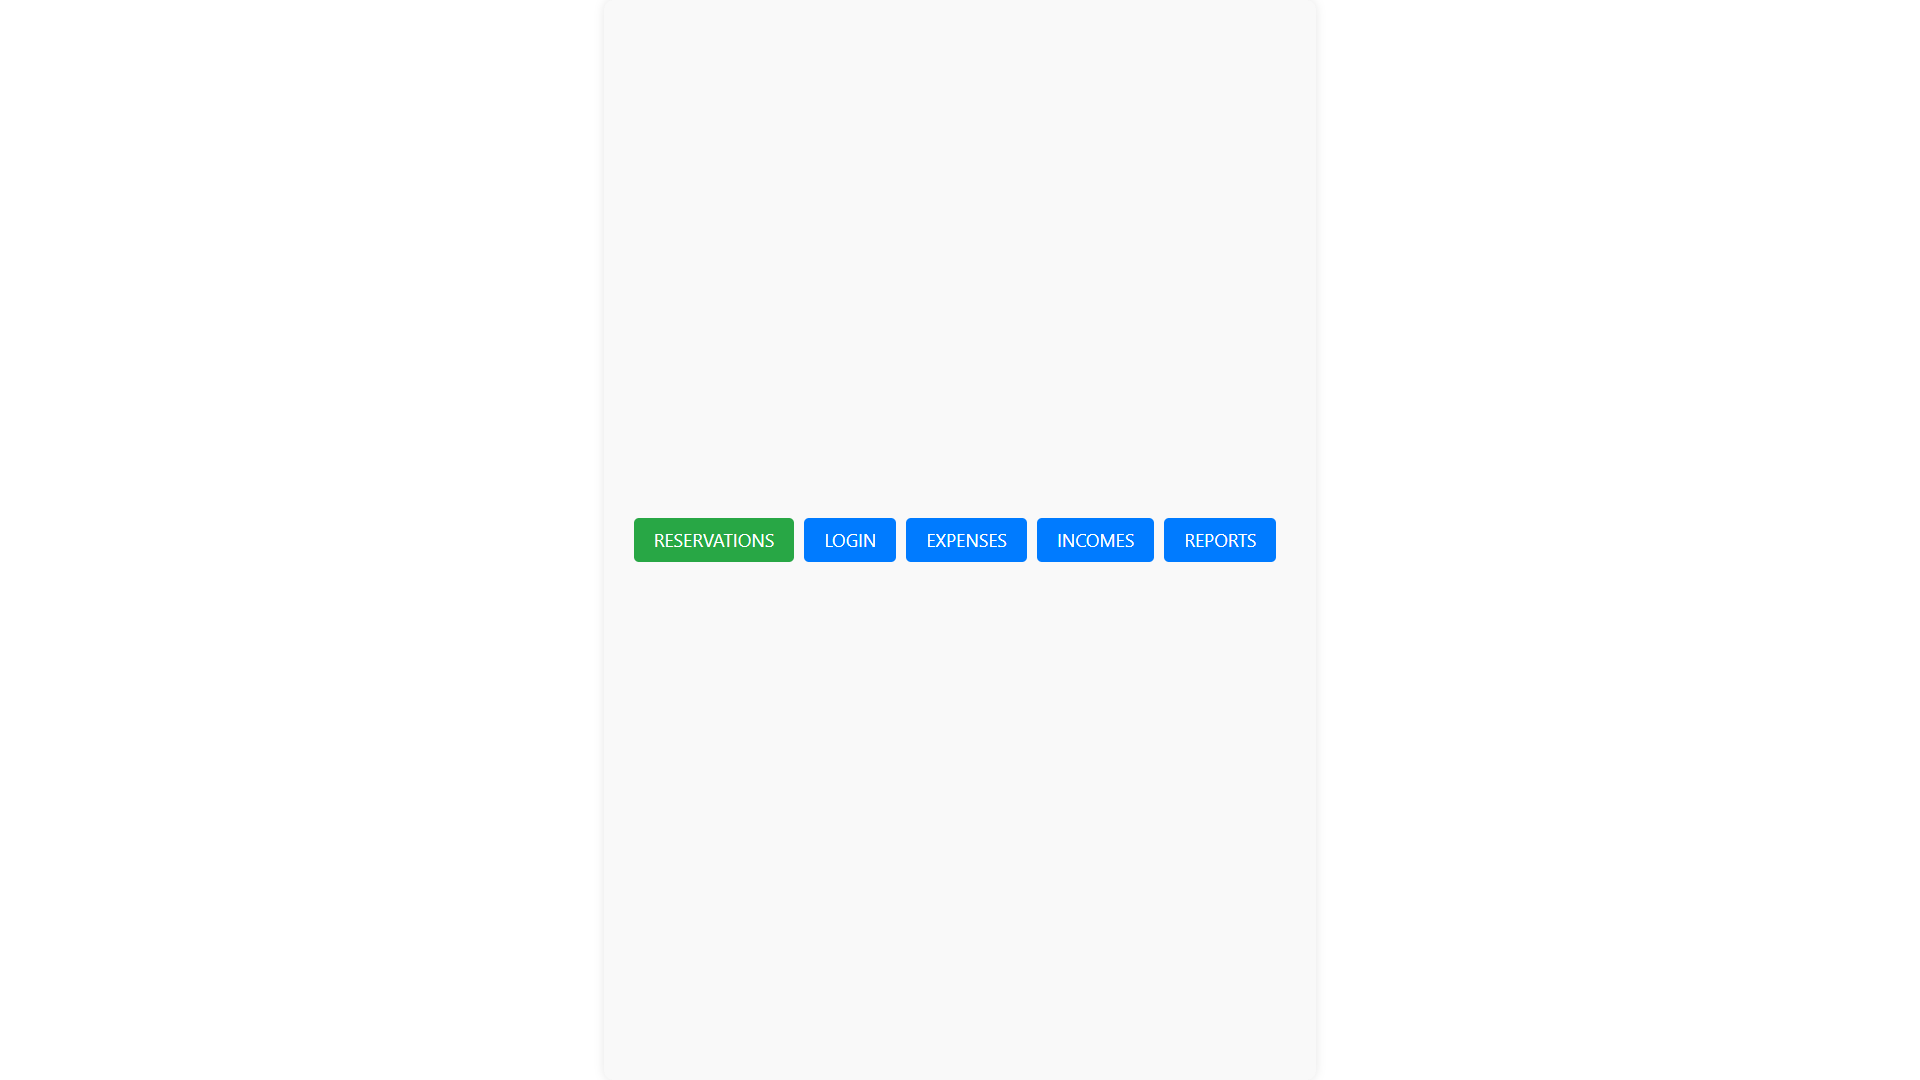
\includegraphics[width=\textwidth]{media/mainPage.png}
\end{center}
\end{minipage}

\newpage
\subsection{Reservations}
\begin{minipage}{\textwidth}
\noindent Po wciśnięciu przycisku \textbf{Reservations}:
\begin{center}
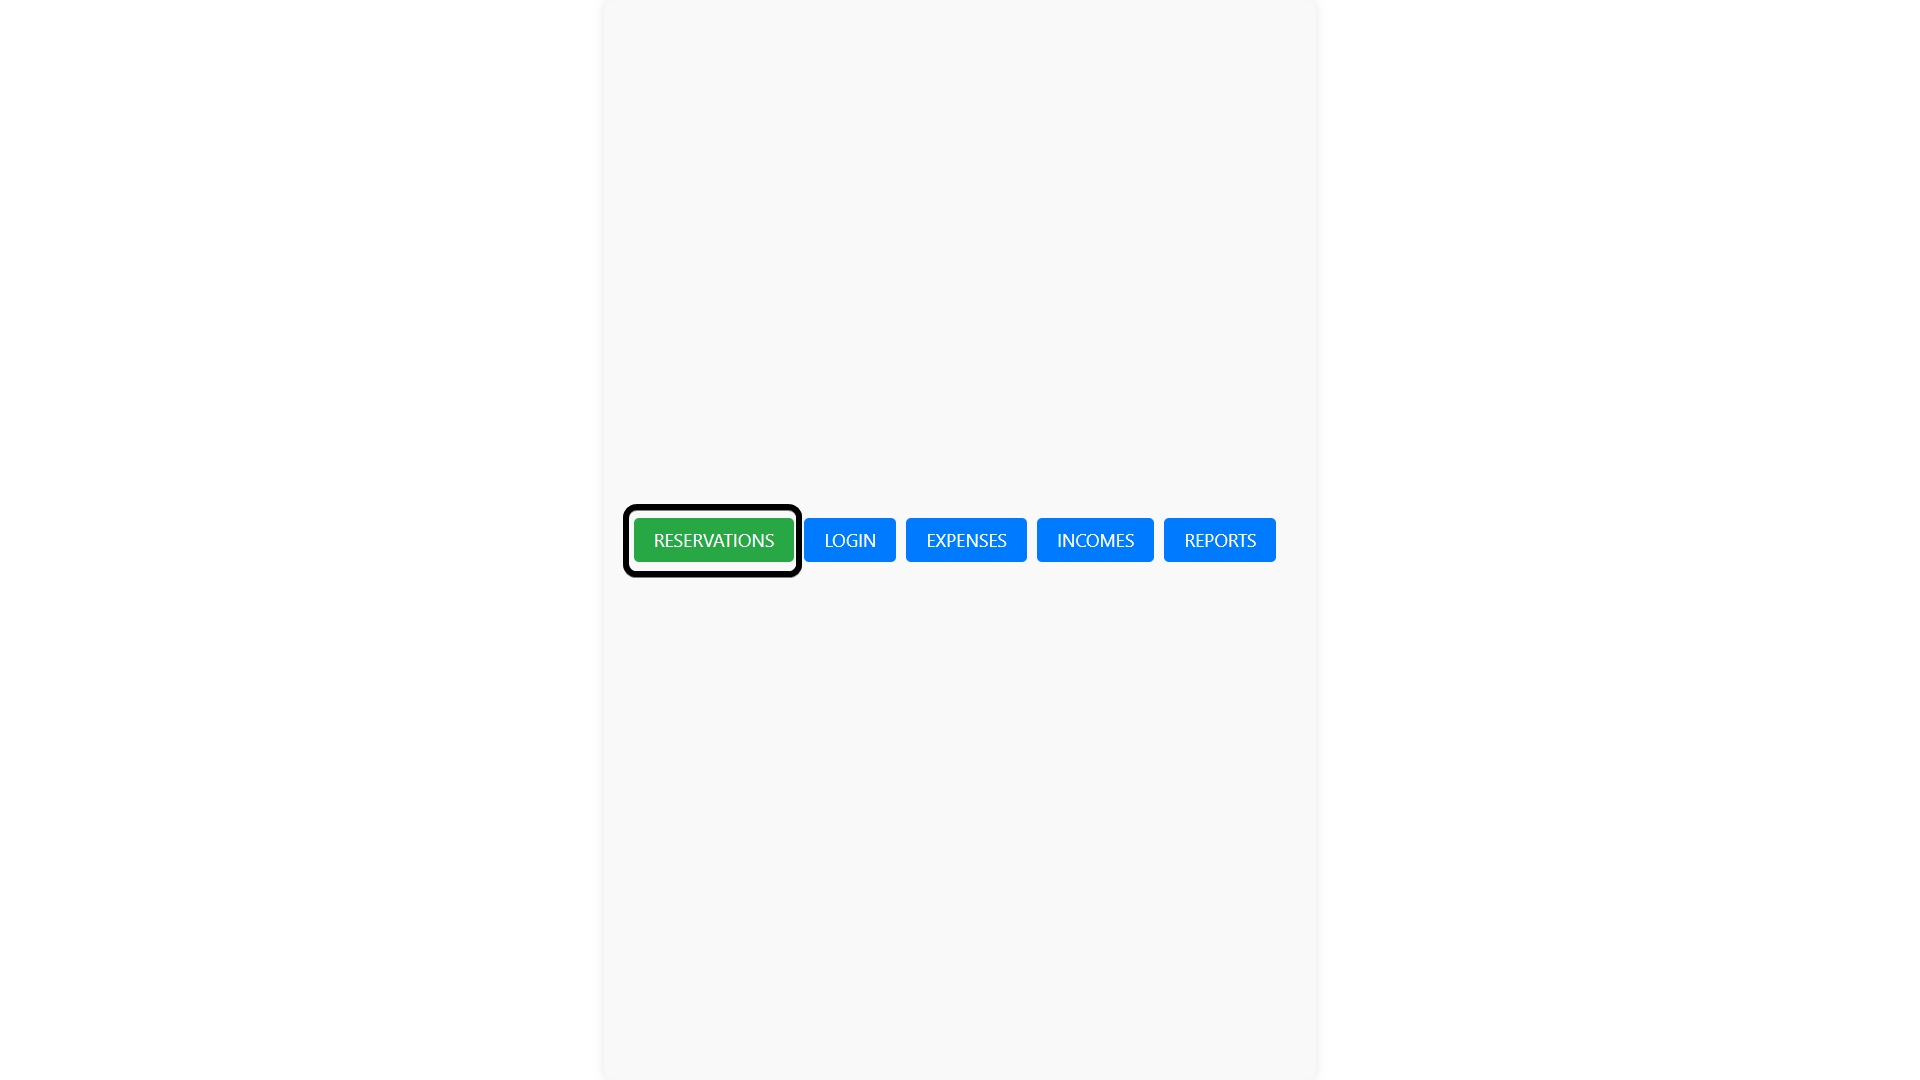
\includegraphics[width=\textwidth]{media/Reservations.png}
\end{center}
\end{minipage}

\begin{minipage}{\textwidth}
\noindent Przenosimy się do panelu rezerwacji:
\begin{center}
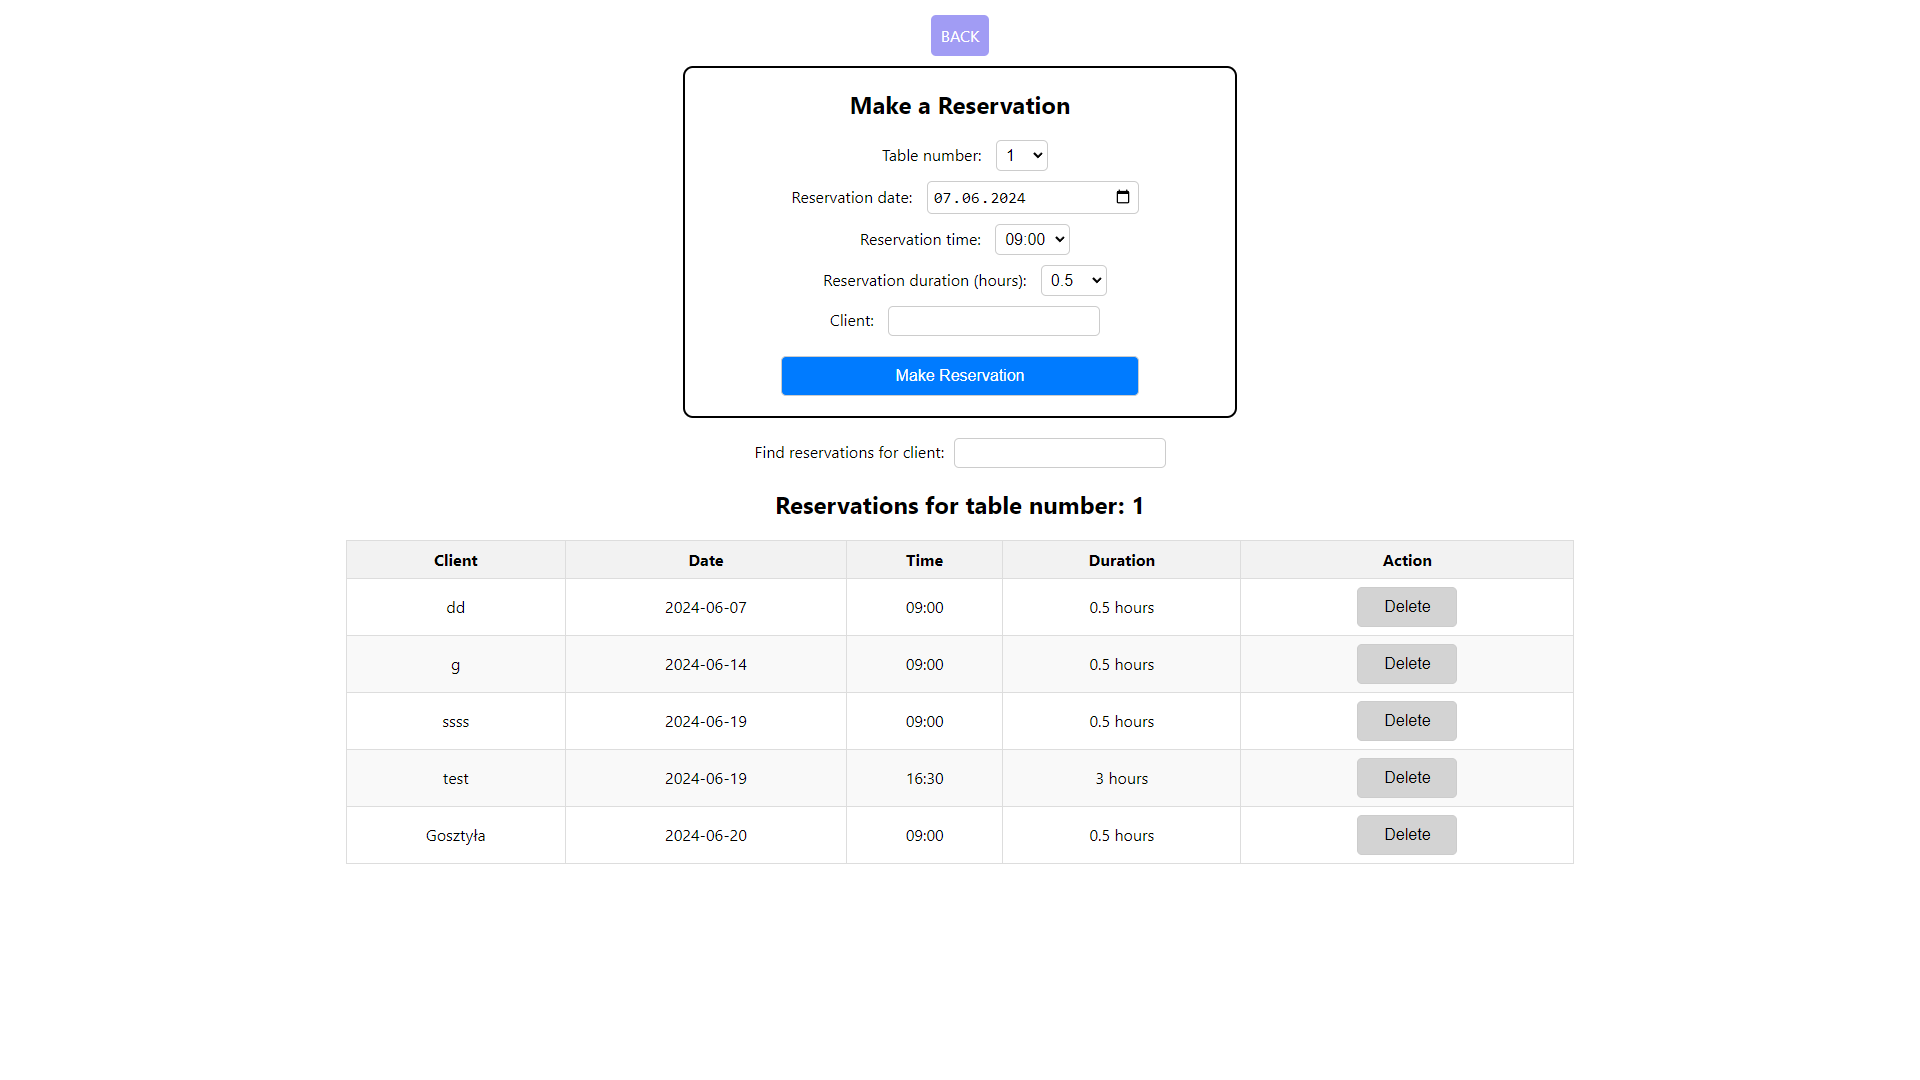
\includegraphics[width=\textwidth]{media/Reservations_in.png}
\end{center}
\end{minipage}

\begin{minipage}{\textwidth}
\noindent Po wypełnieniu danych o rezerwacji klienta, możemy spóbować dodać taką rezerwację, za pomocą przycisku \textbf{Make Reservation}:
\begin{center}
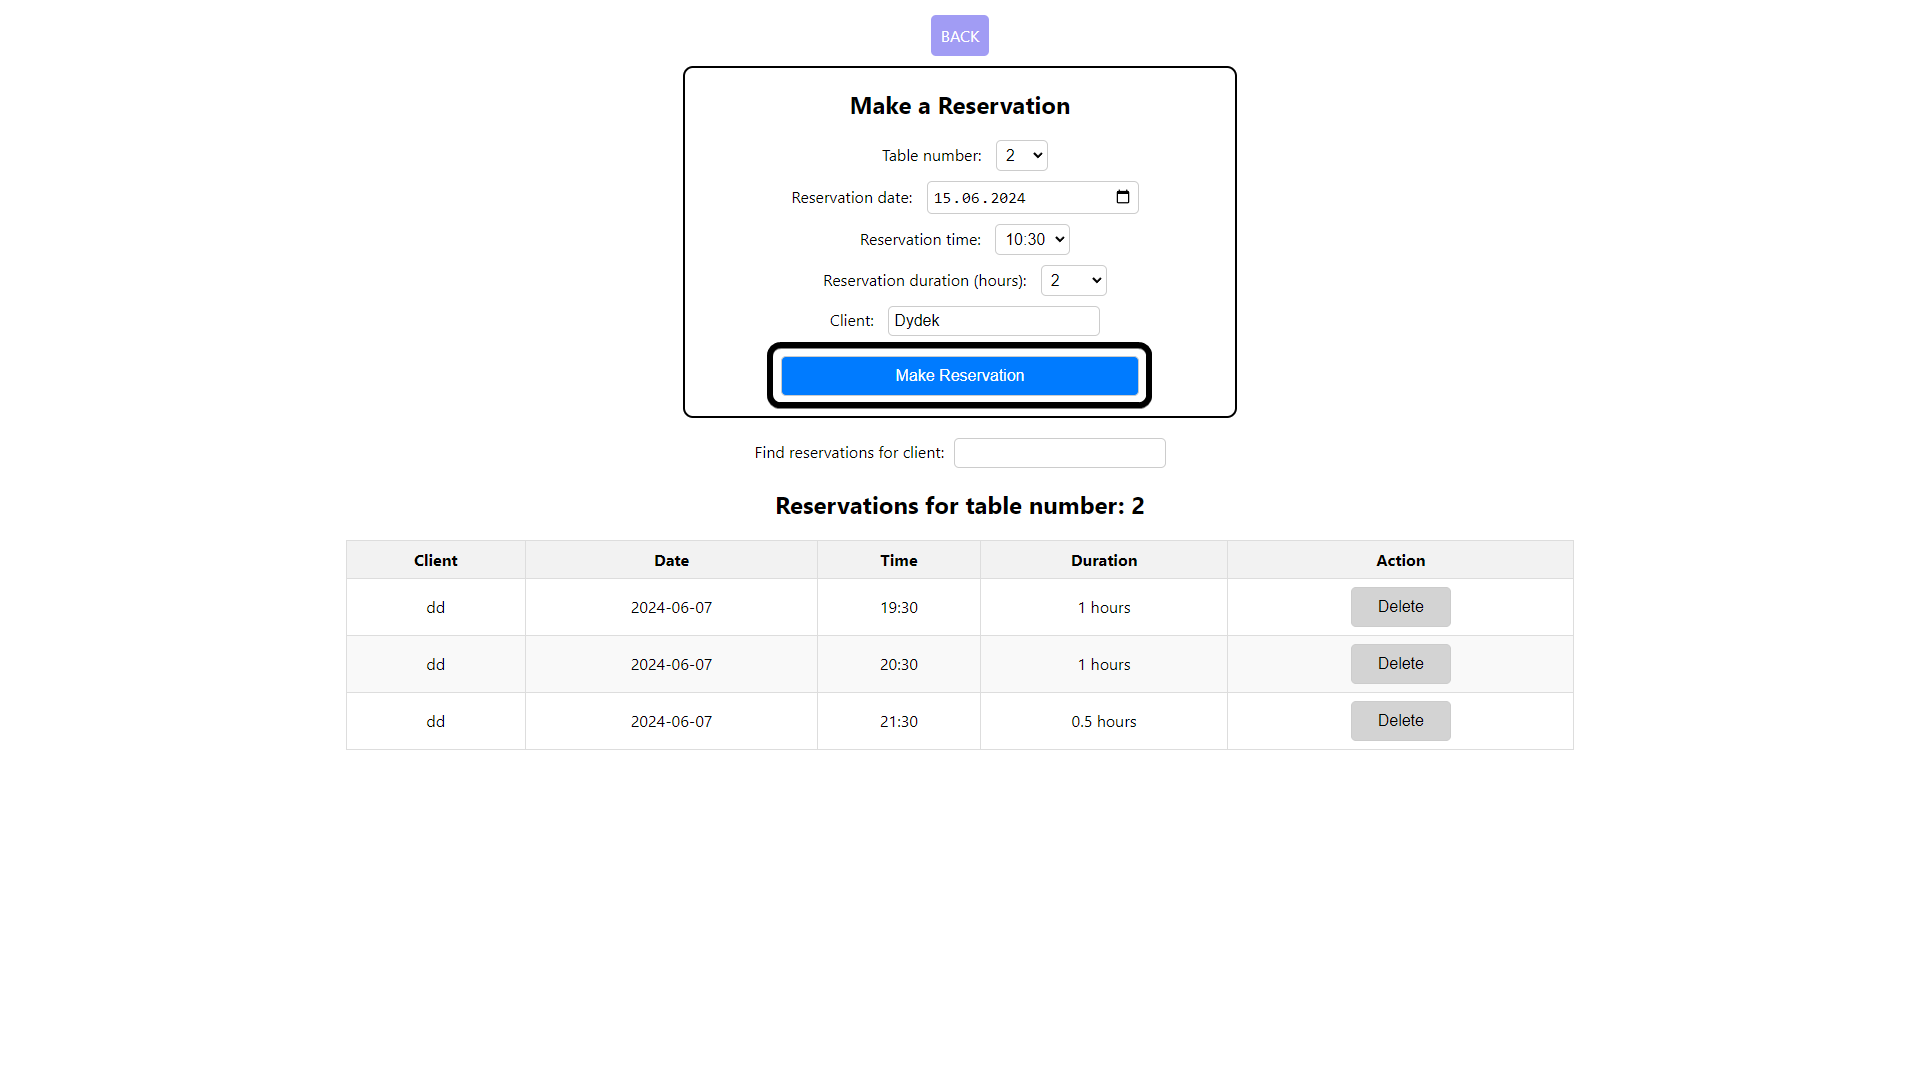
\includegraphics[width=\textwidth]{media/Reservations_makeReservations.png}
\end{center}
\end{minipage}

\begin{minipage}{\textwidth}
\noindent Jeśli dane rezerwacji są poprawne, dostaniemy komunikat o poprawnym dodaniu rezerwacji:
\begin{center}
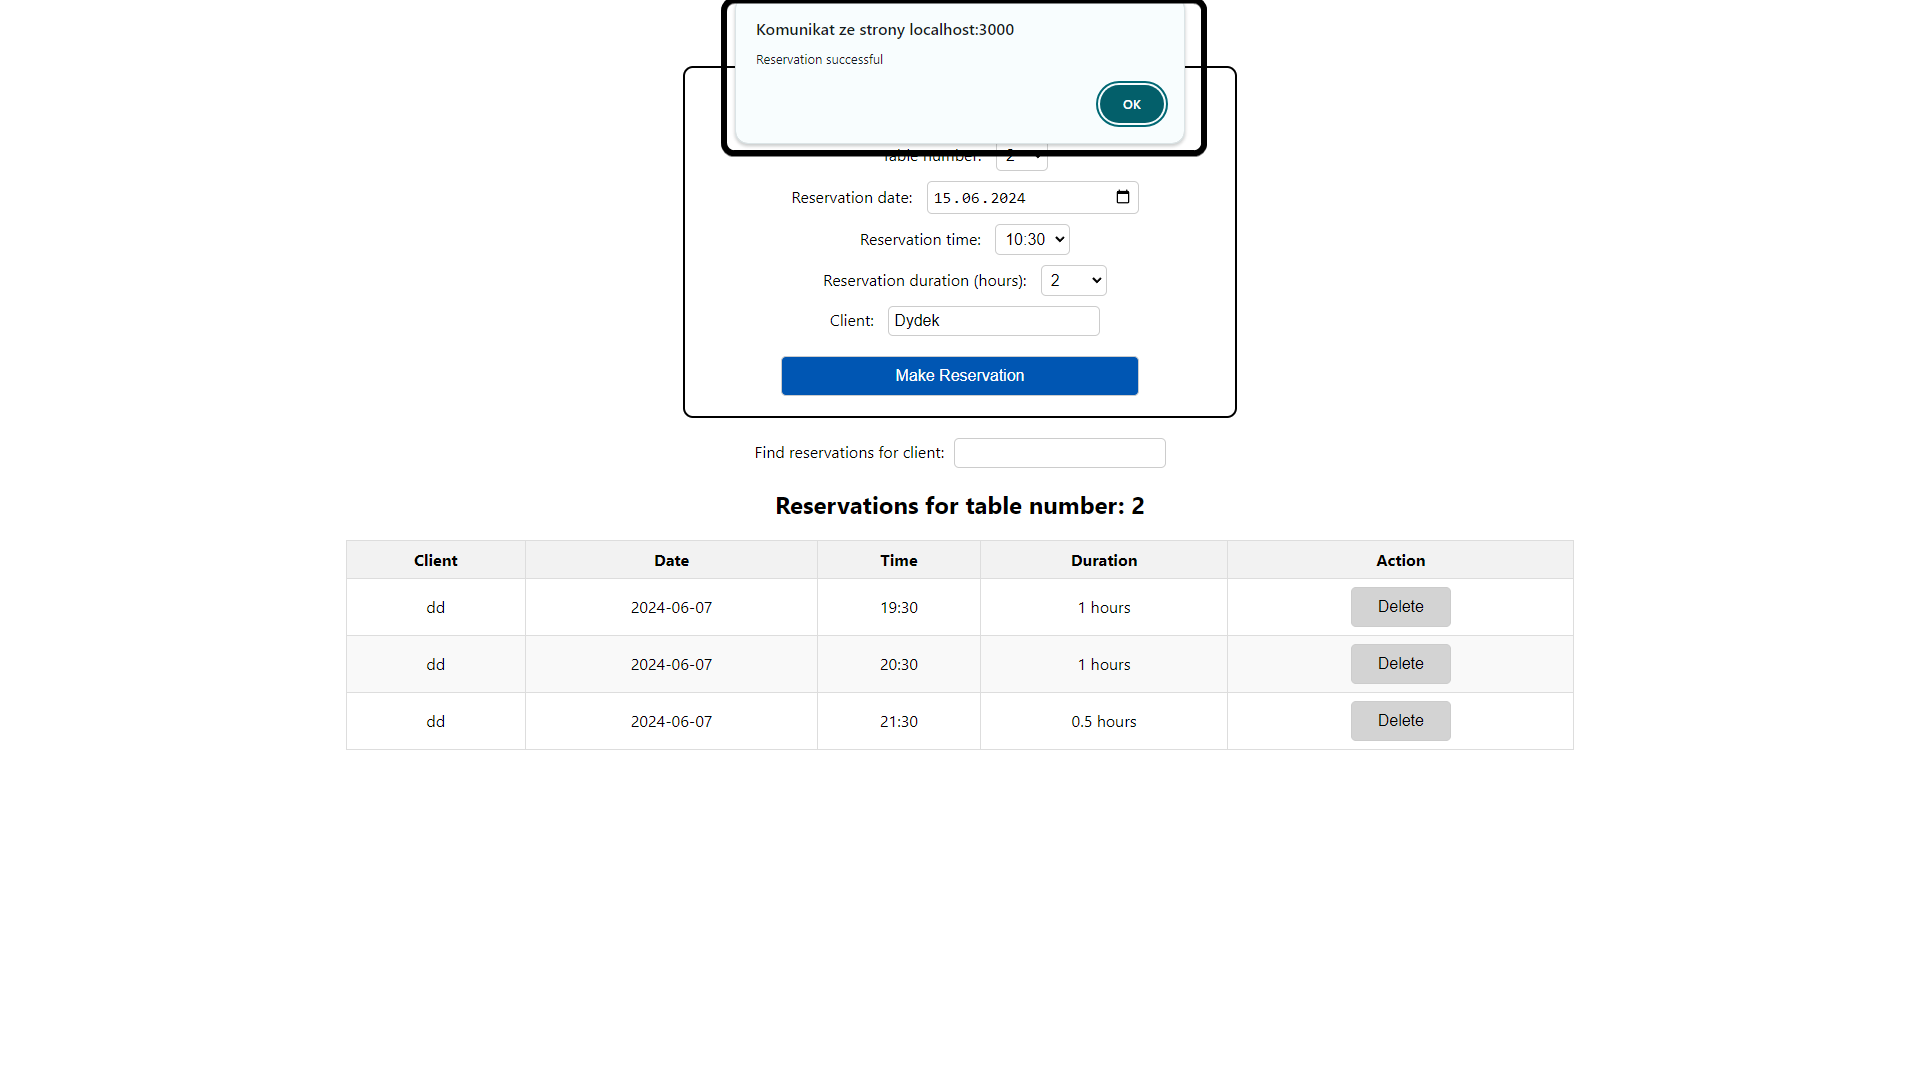
\includegraphics[width=\textwidth]{media/Reservations_makeReservationsAlert.png}
\end{center}
\end{minipage}

\begin{minipage}{\textwidth}
\noindent Rezerwacja następnie będzie dostępna w widoku rezerwacji dla wybranego stolika:
\begin{center}
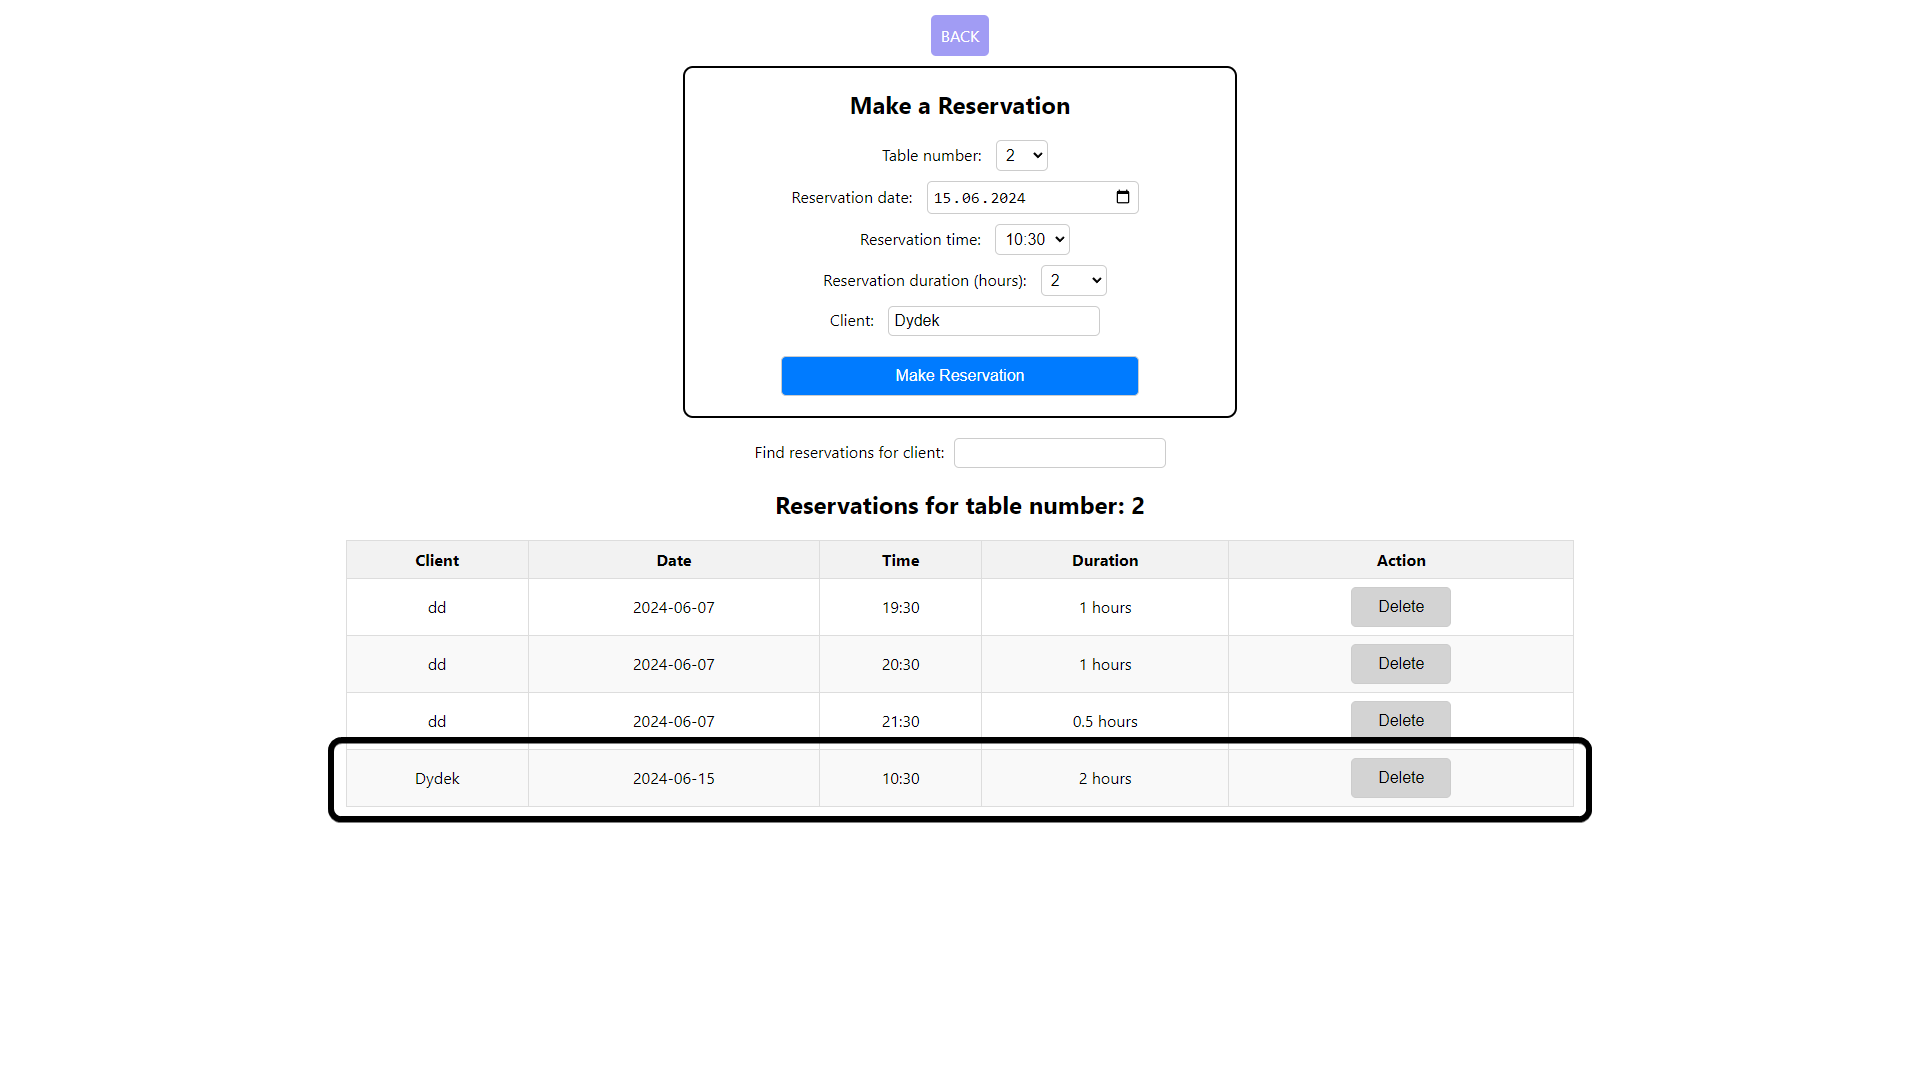
\includegraphics[width=\textwidth]{media/Reservations_addedReservation.png}
\end{center}
\end{minipage}

\begin{minipage}{\textwidth}
\noindent Jeśli wybraliśmy termin rezerwacji w przeszłości, to nie będziemy mogli dokonać rezerwacji:
\begin{center}
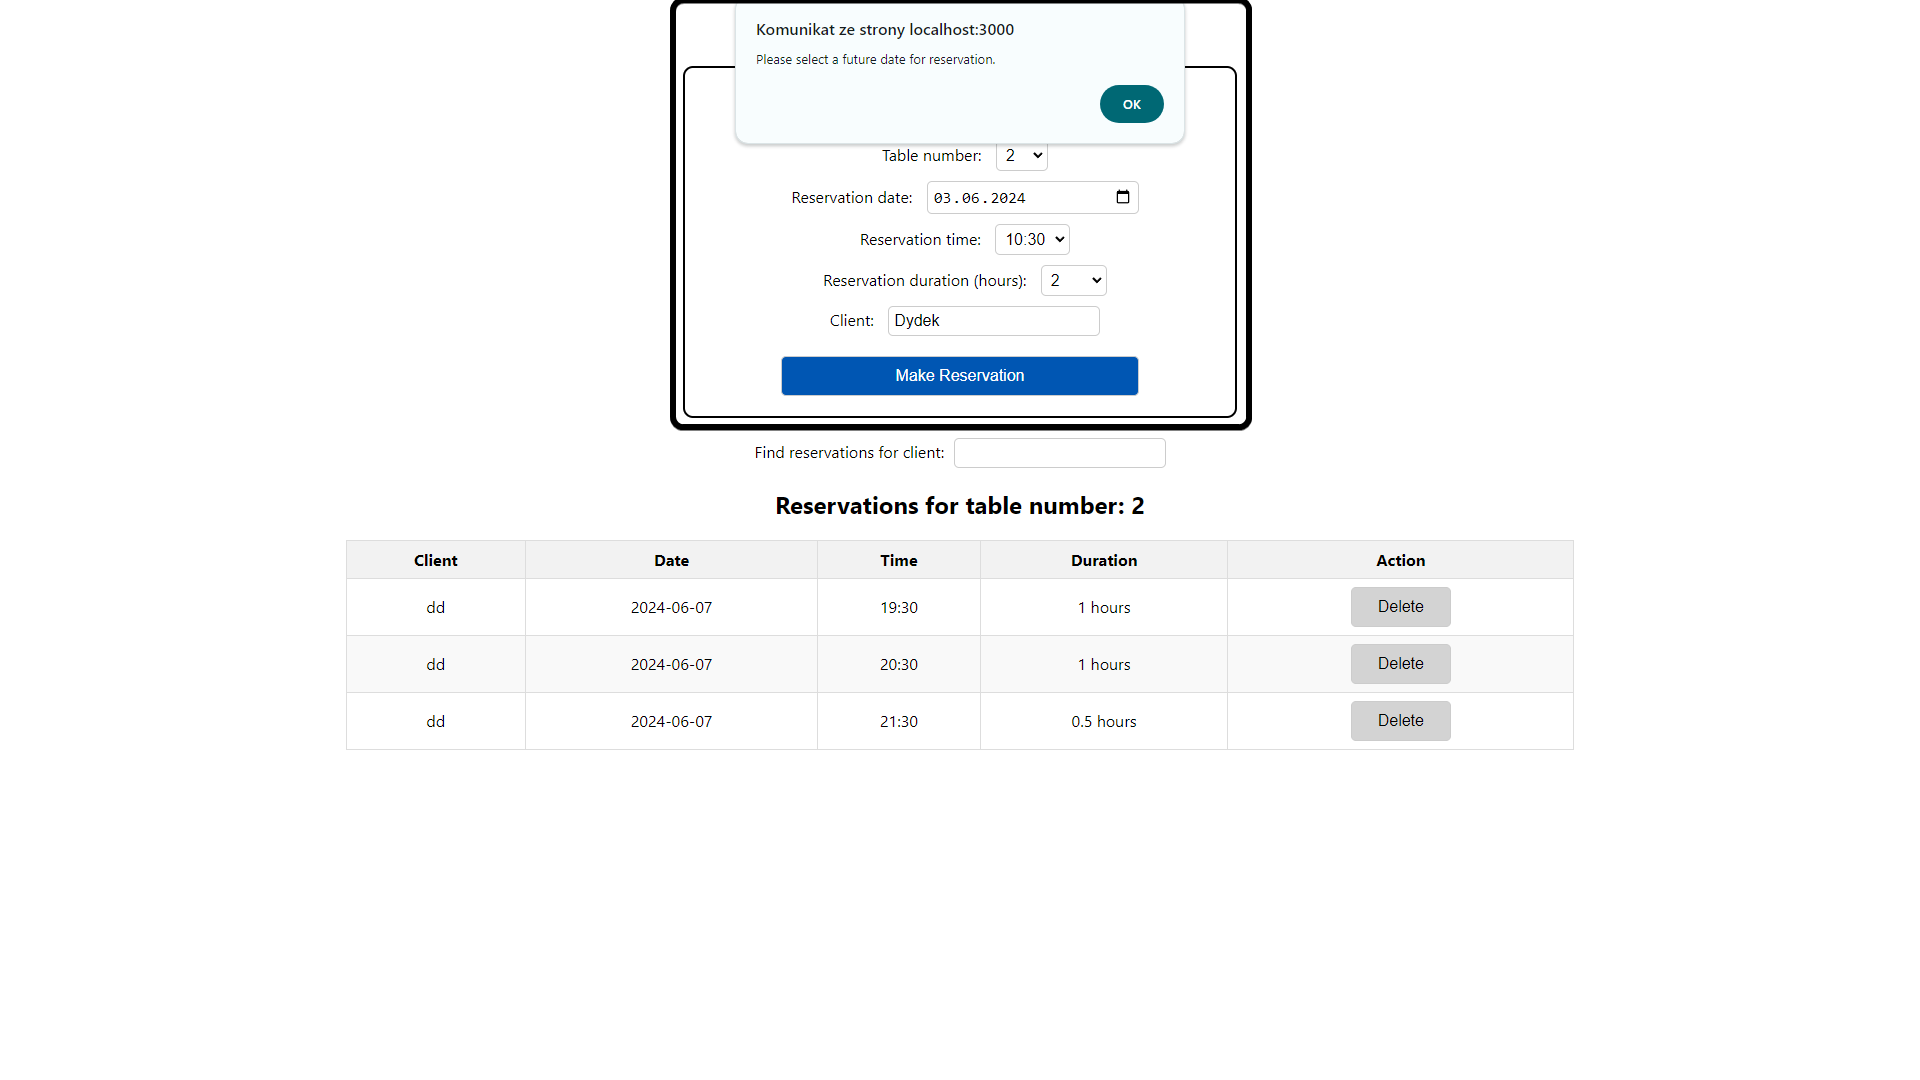
\includegraphics[width=\textwidth]{media/Reservations_previousDate.png}
\end{center}
\end{minipage}

\begin{minipage}{\textwidth}
\noindent Jeśli wybraliśmy termin rezerwacji, który kończy się po zamknięciu rezerwacji, dostaniemy komunikat:
\begin{center}
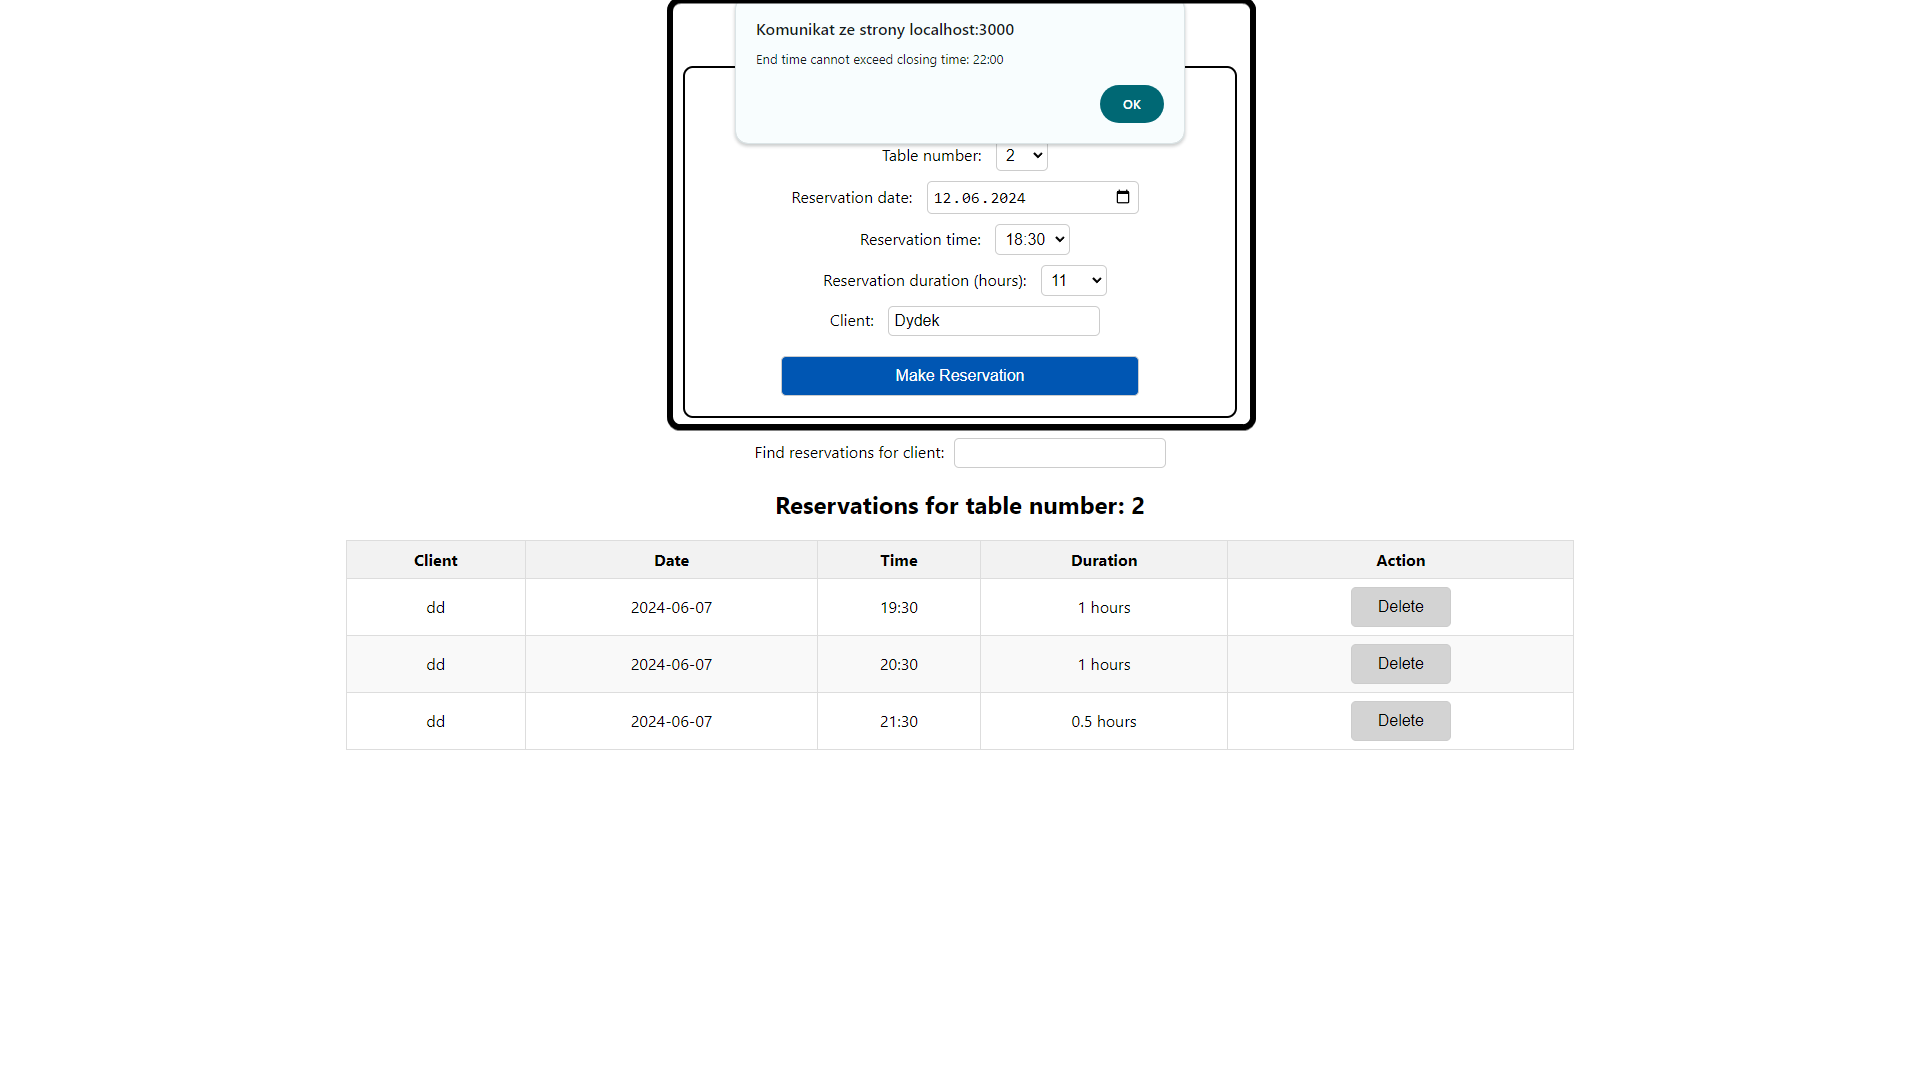
\includegraphics[width=\textwidth]{media/Reservations_tooLong.png}
\end{center}
\end{minipage}

\begin{minipage}{\textwidth}
\noindent Jeśli wybraliśmy termin rezerwacji, który jakkolwiek nachodzi na inną rezerwację, dokonaną na ten sam stolik, dostaniemy komunikat:
\begin{center}
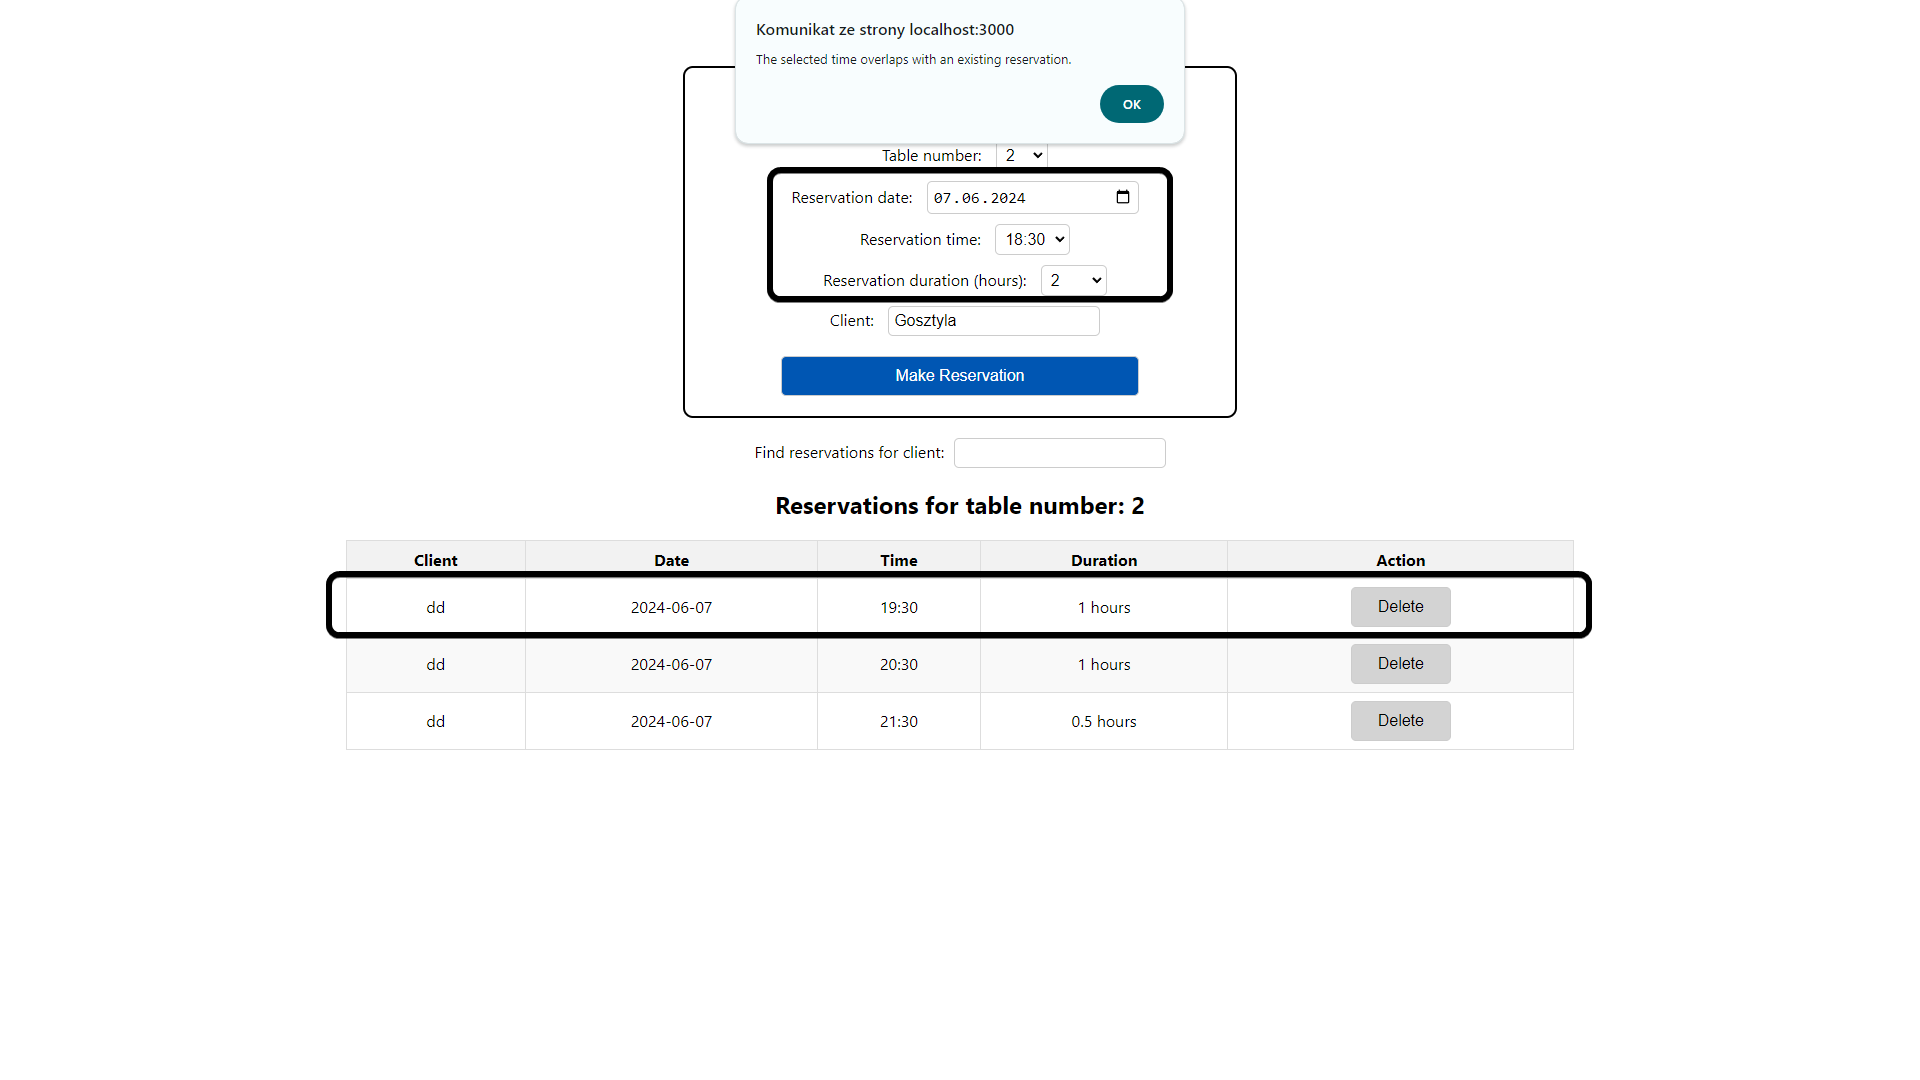
\includegraphics[width=\textwidth]{media/Reservations_overlap.png}
\end{center}
\end{minipage}

\begin{minipage}{\textwidth}
\noindent Mamy również możliwość usunięcia rezerwacji:
\begin{center}
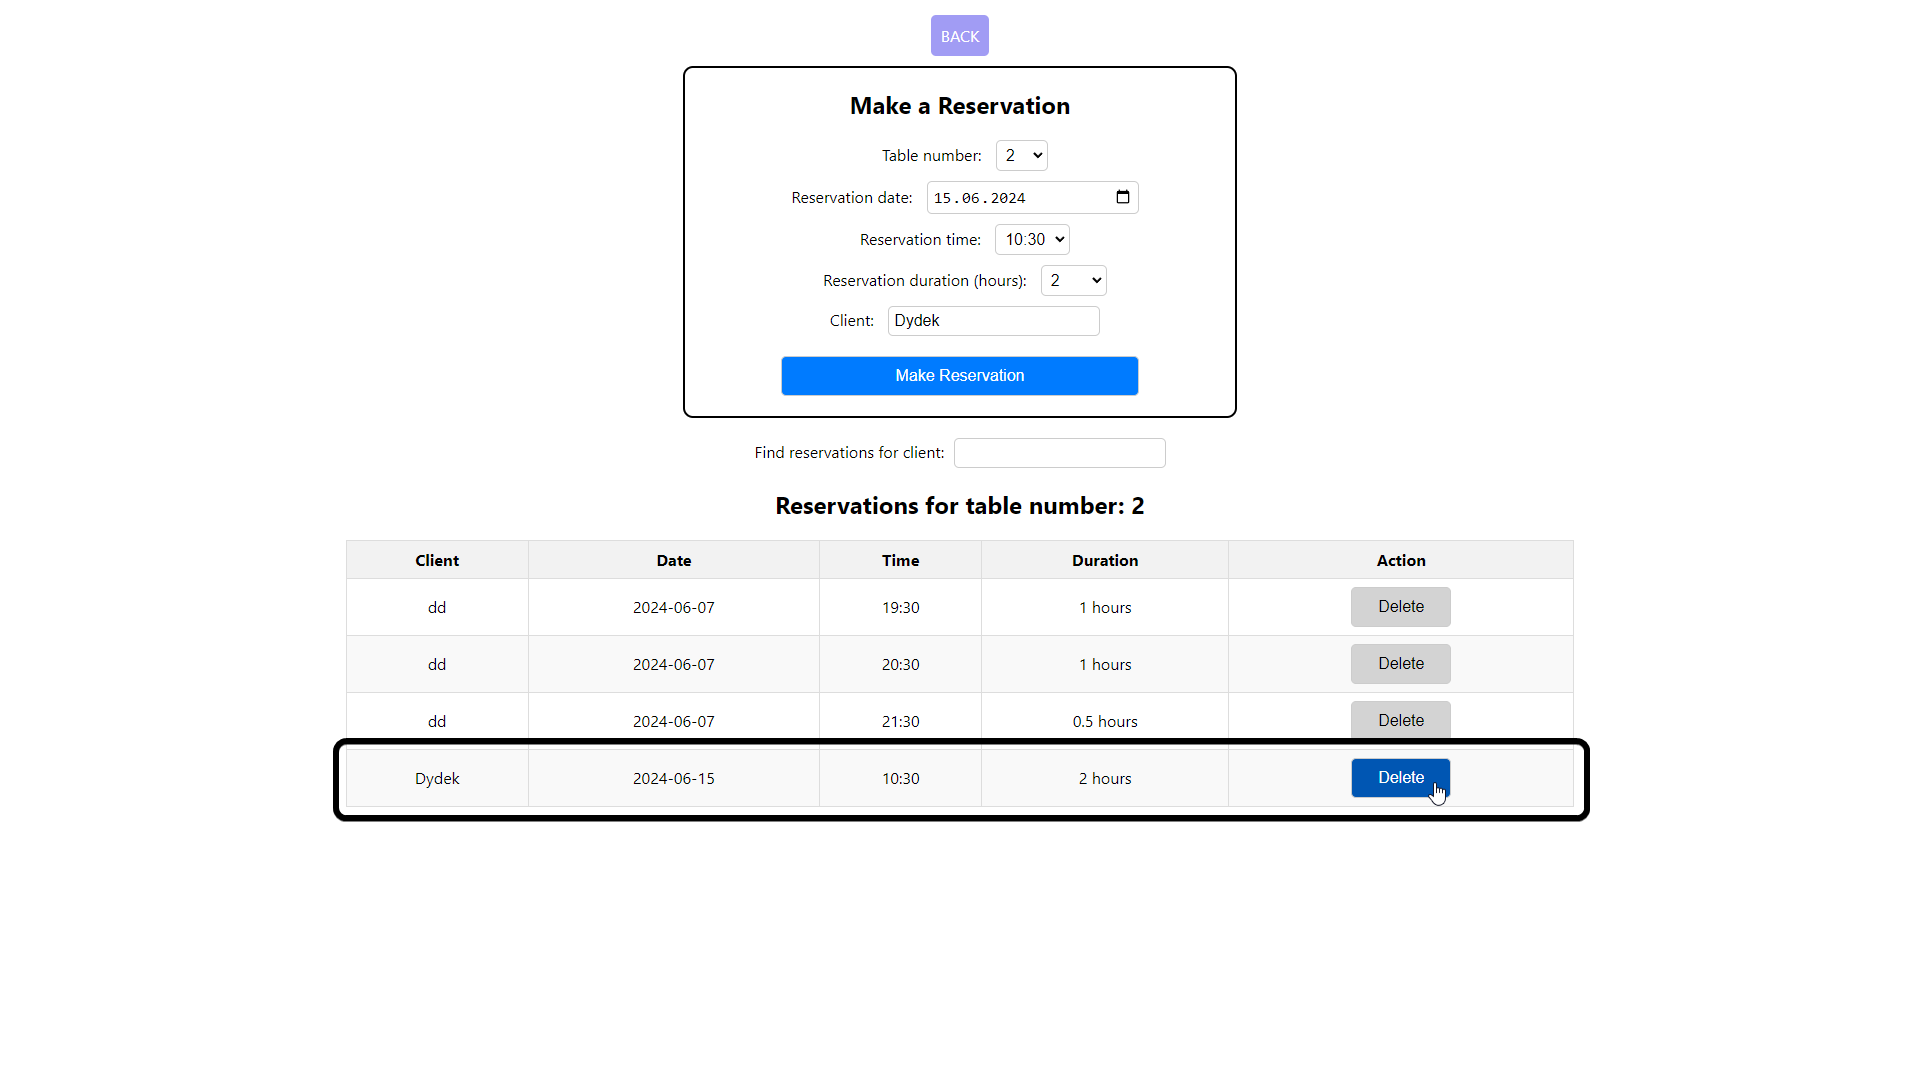
\includegraphics[width=\textwidth]{media/Reservation_delete.png}
\end{center}
\end{minipage}

\begin{minipage}{\textwidth}
\noindent Po usunięciu dostaniemy komunikat:
\begin{center}
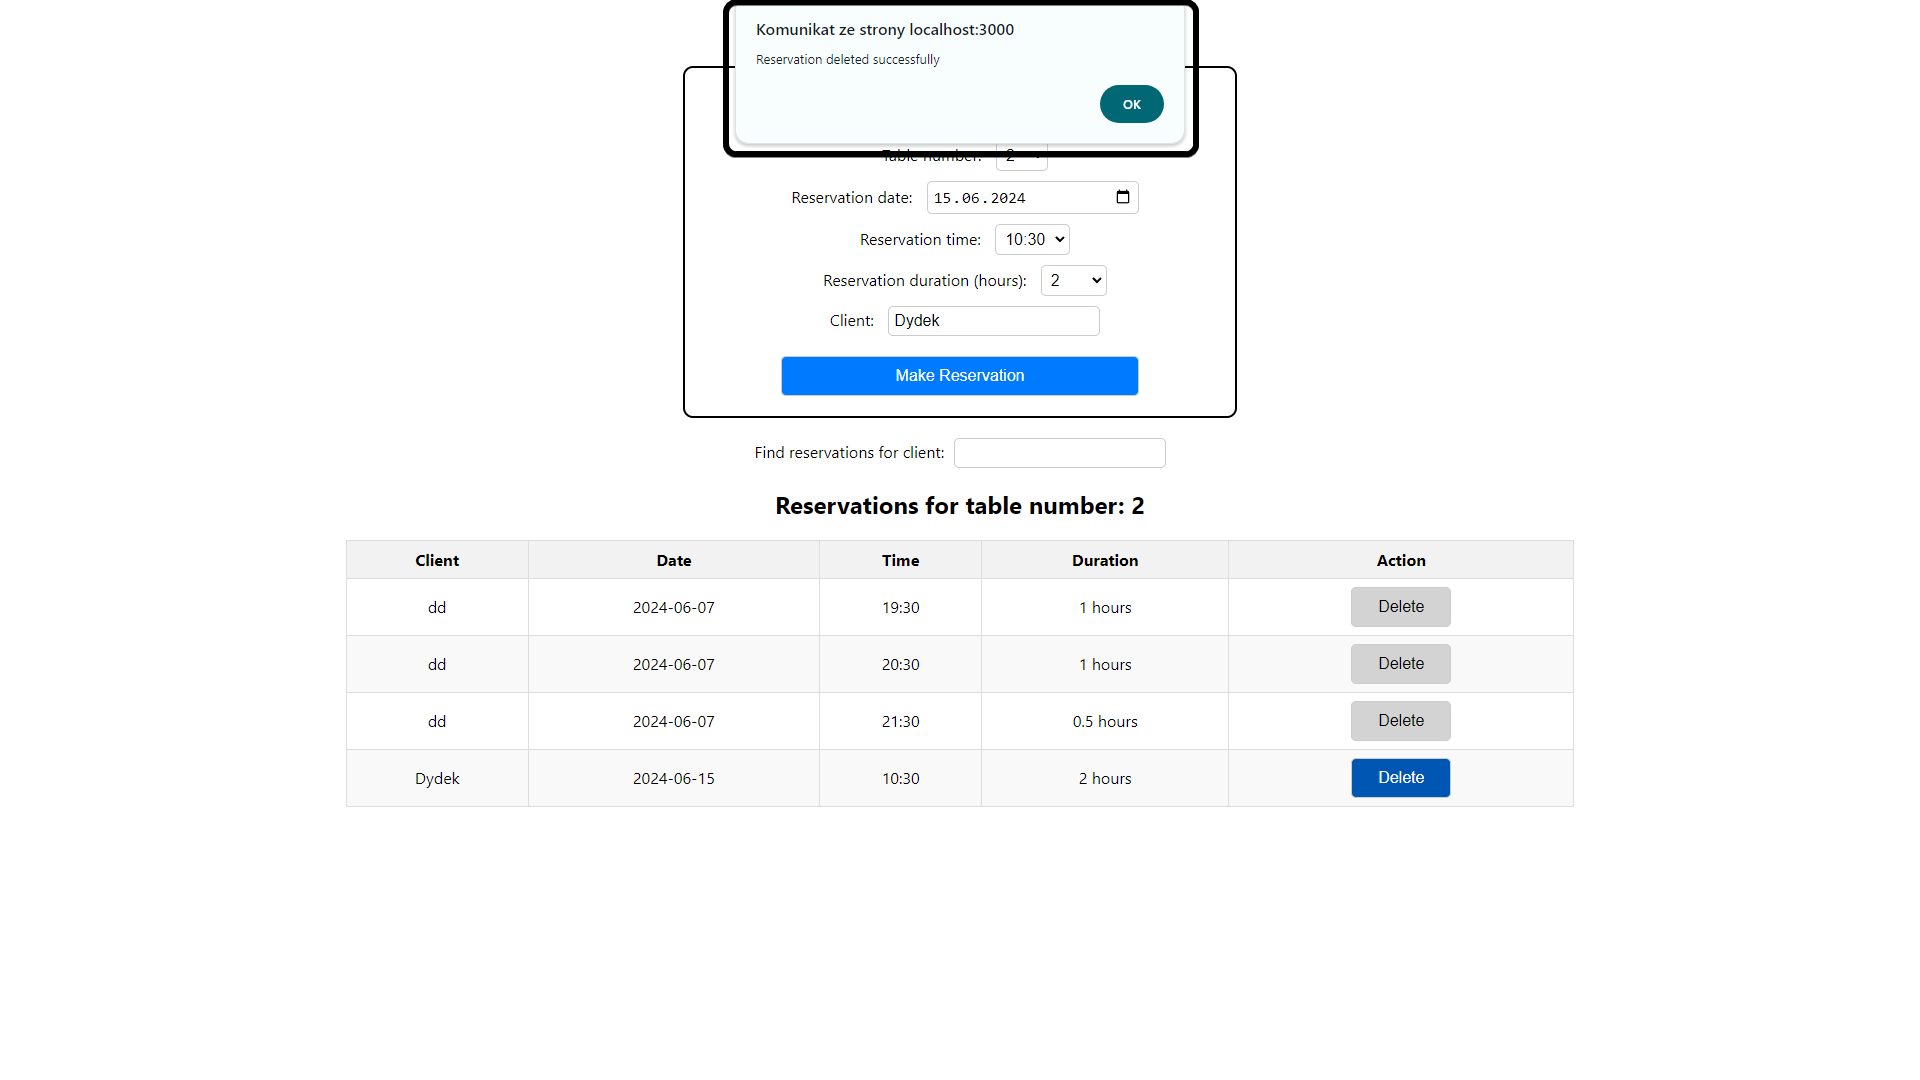
\includegraphics[width=\textwidth]{media/Reservations_delete_successfull.png}
\end{center}
\end{minipage}

\begin{minipage}{\textwidth}
\noindent Mamy również możliwość wyszukania wszystkich rezerwacji, dla danego klienta:
\begin{center}
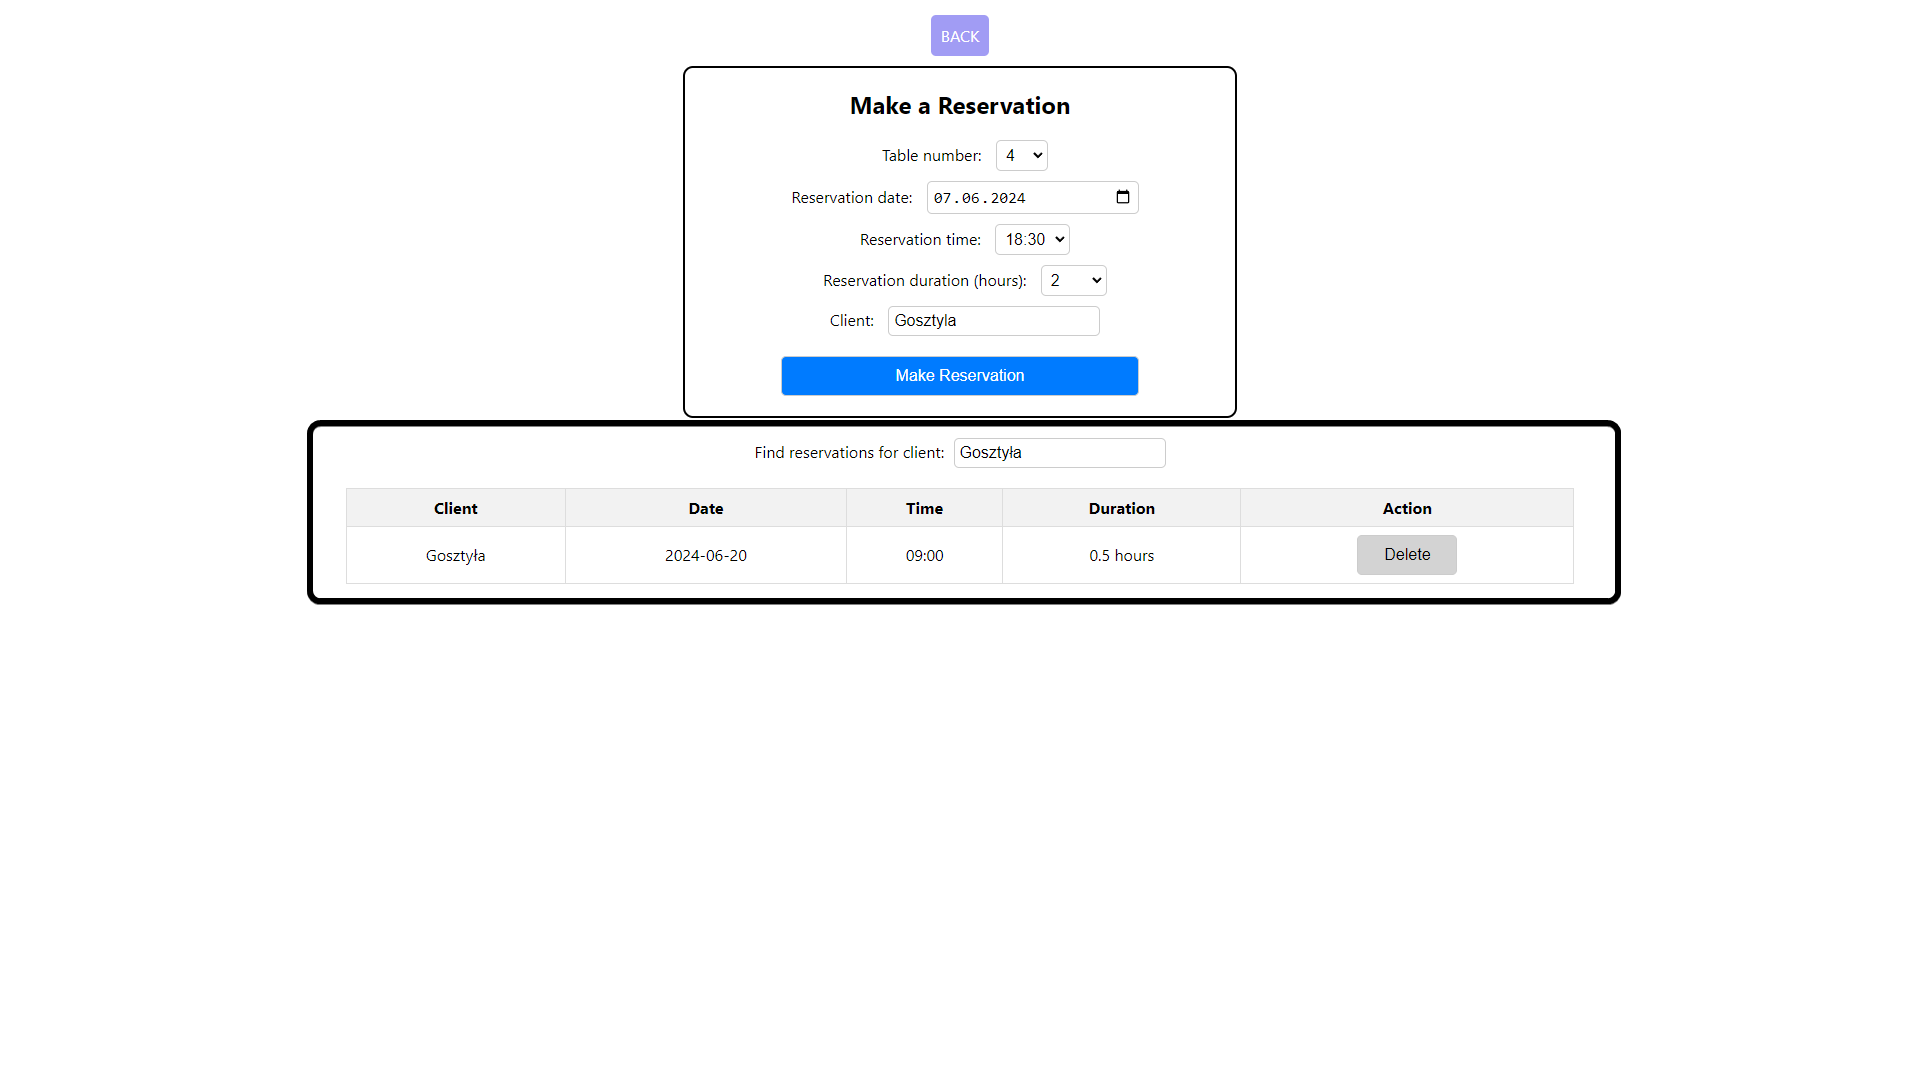
\includegraphics[width=\textwidth]{media/Reservations_searchClient.png}
\end{center}
\end{minipage}

\newpage
\subsection{Login}
\begin{minipage}{\textwidth}
\noindent Po wciśnięciu przycisku \textbf{Login}:
\begin{center}
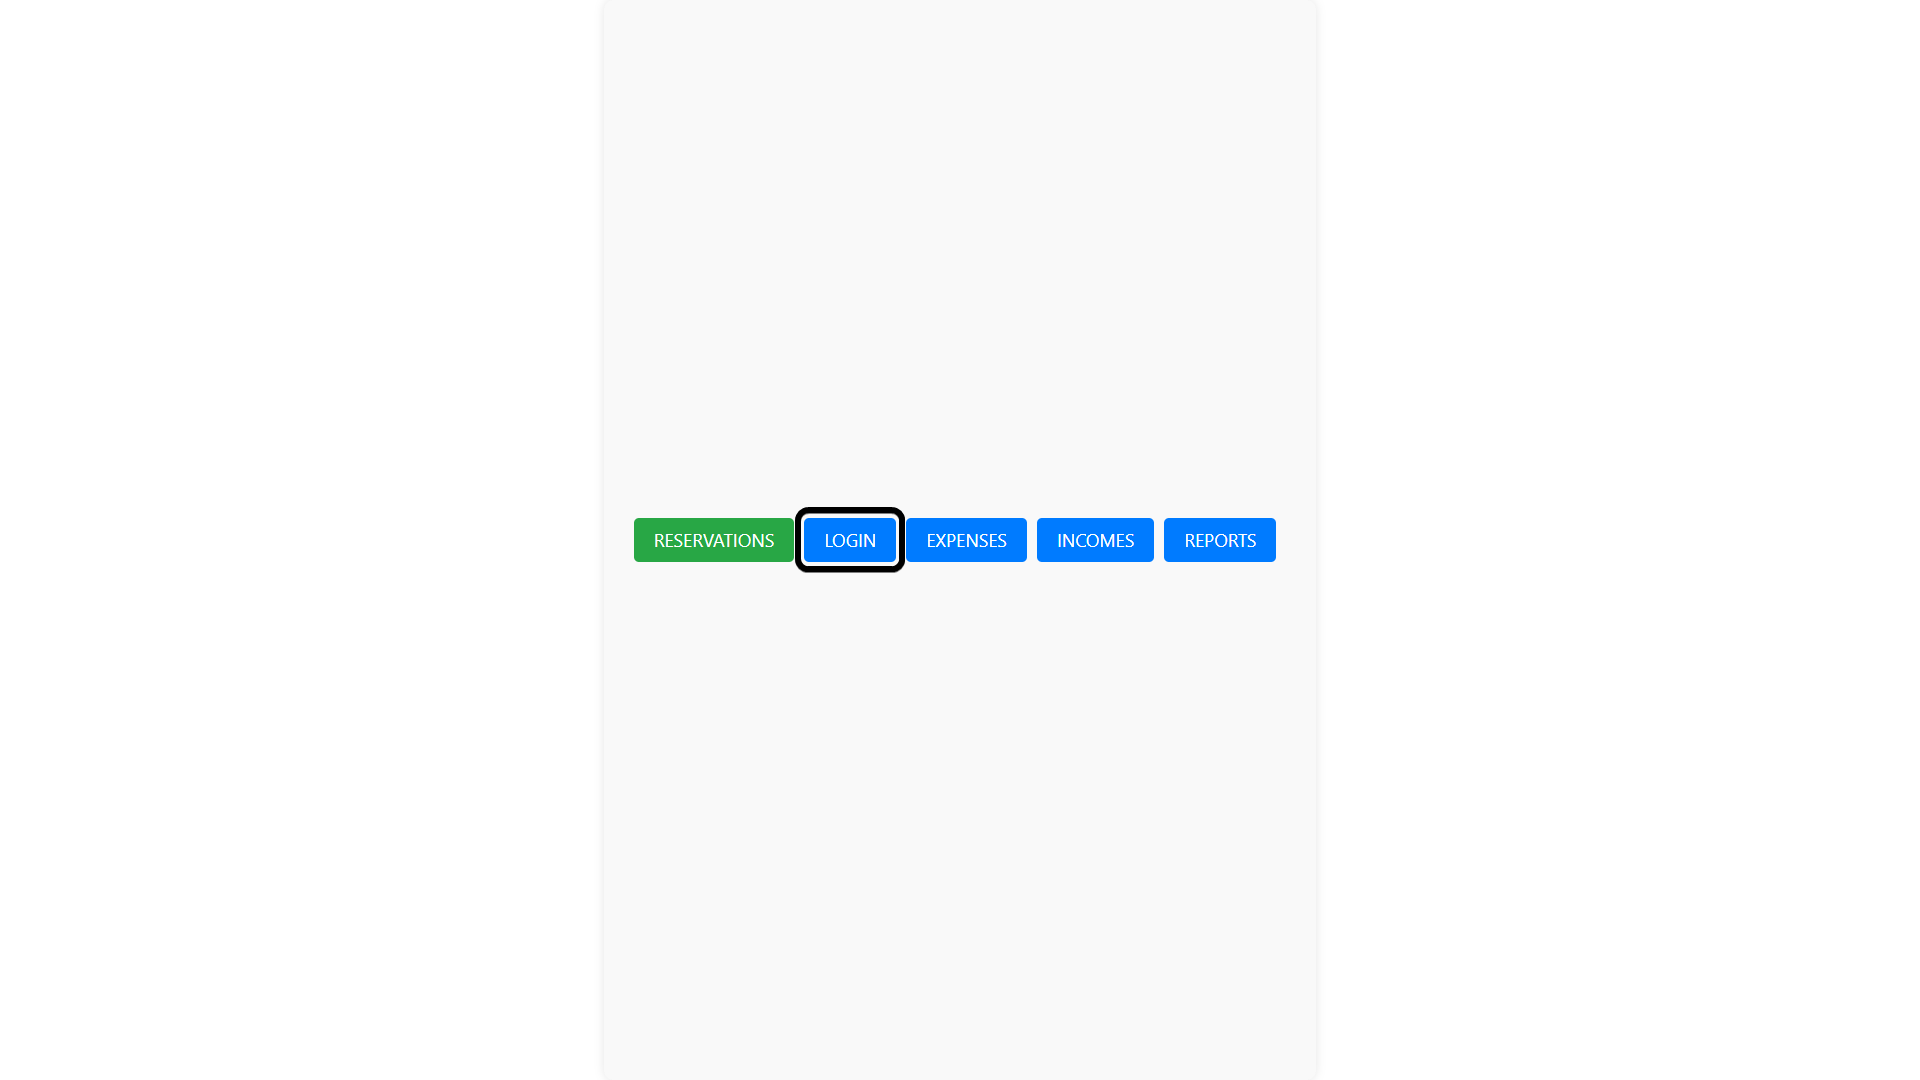
\includegraphics[width=\textwidth]{media/Login.png}
\end{center}
\end{minipage}

\begin{minipage}{\textwidth}
\noindent Przenosimy się do panelu logowania:
\begin{center}
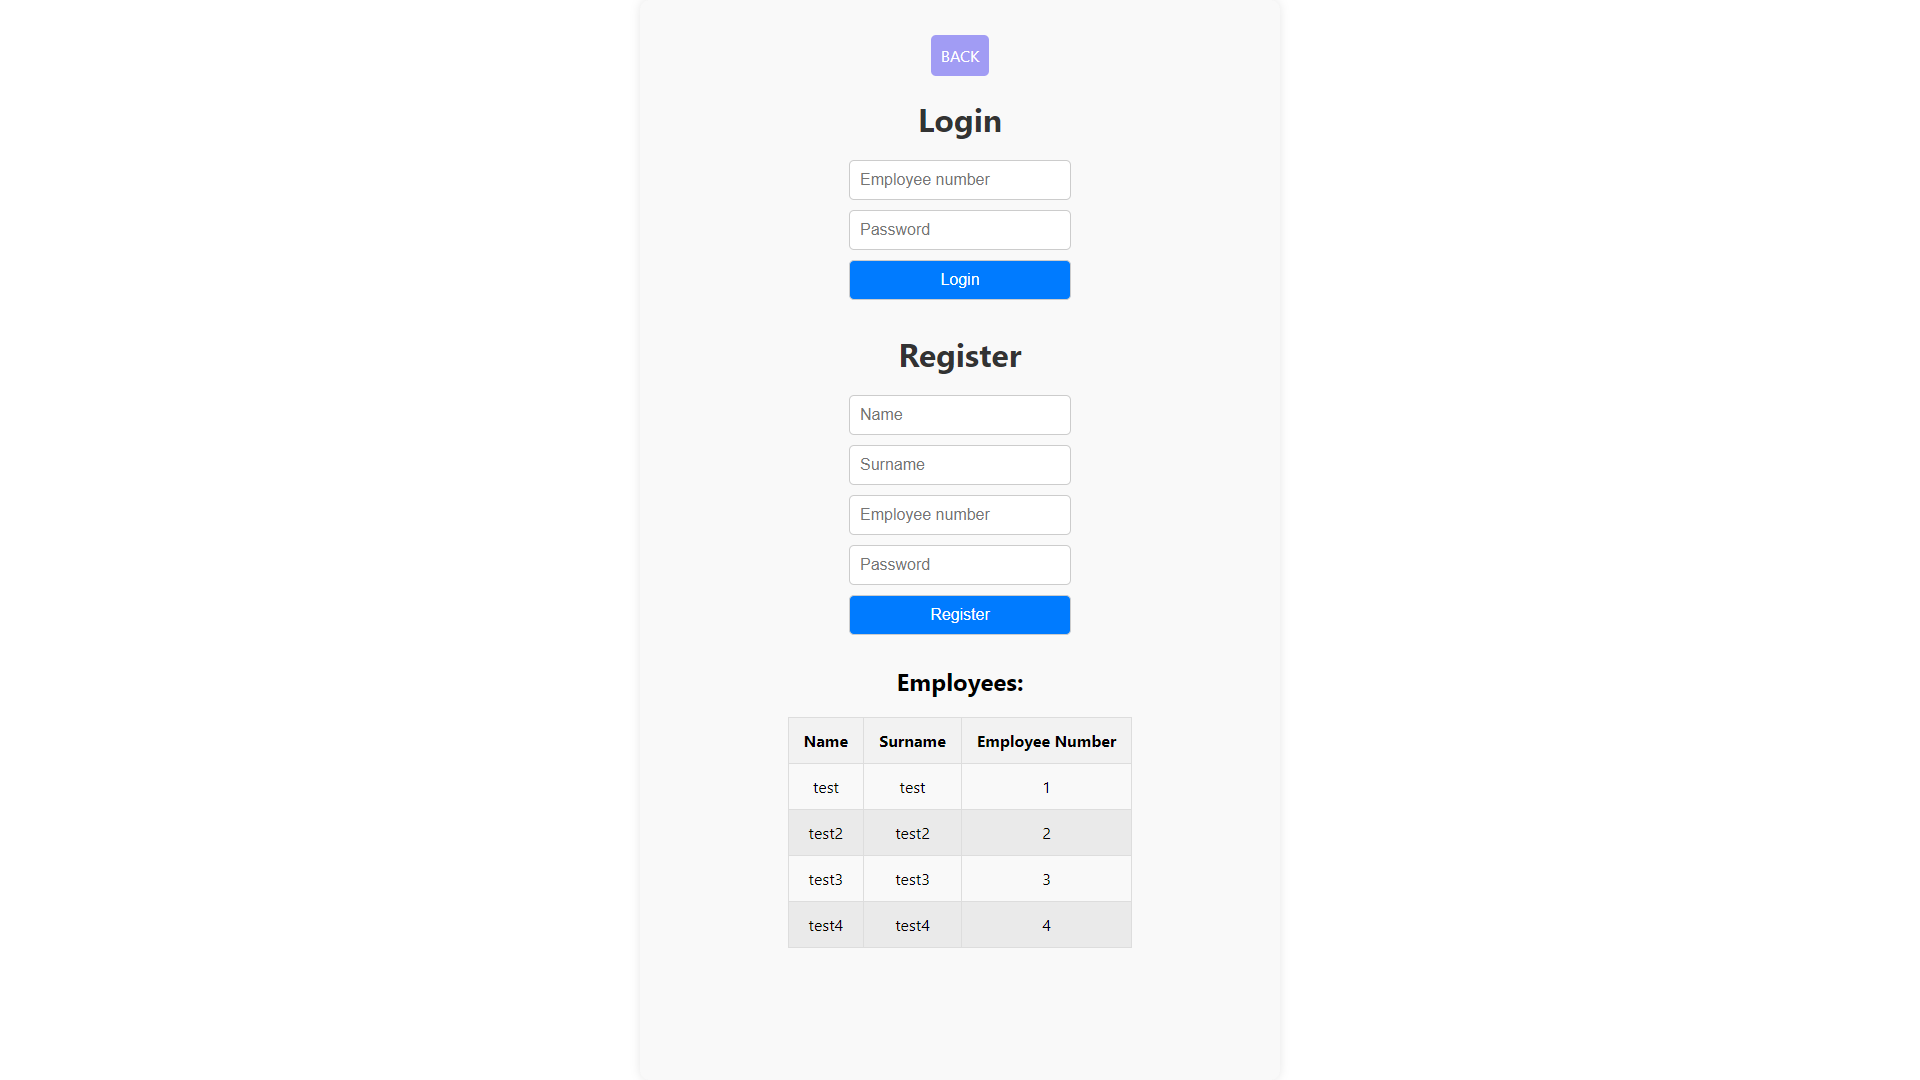
\includegraphics[width=\textwidth]{media/Login_in.png}
\end{center}
\end{minipage}

\begin{minipage}{\textwidth}
\noindent Możemy zalogować się na istniejące konto pracownicze:
\begin{center}
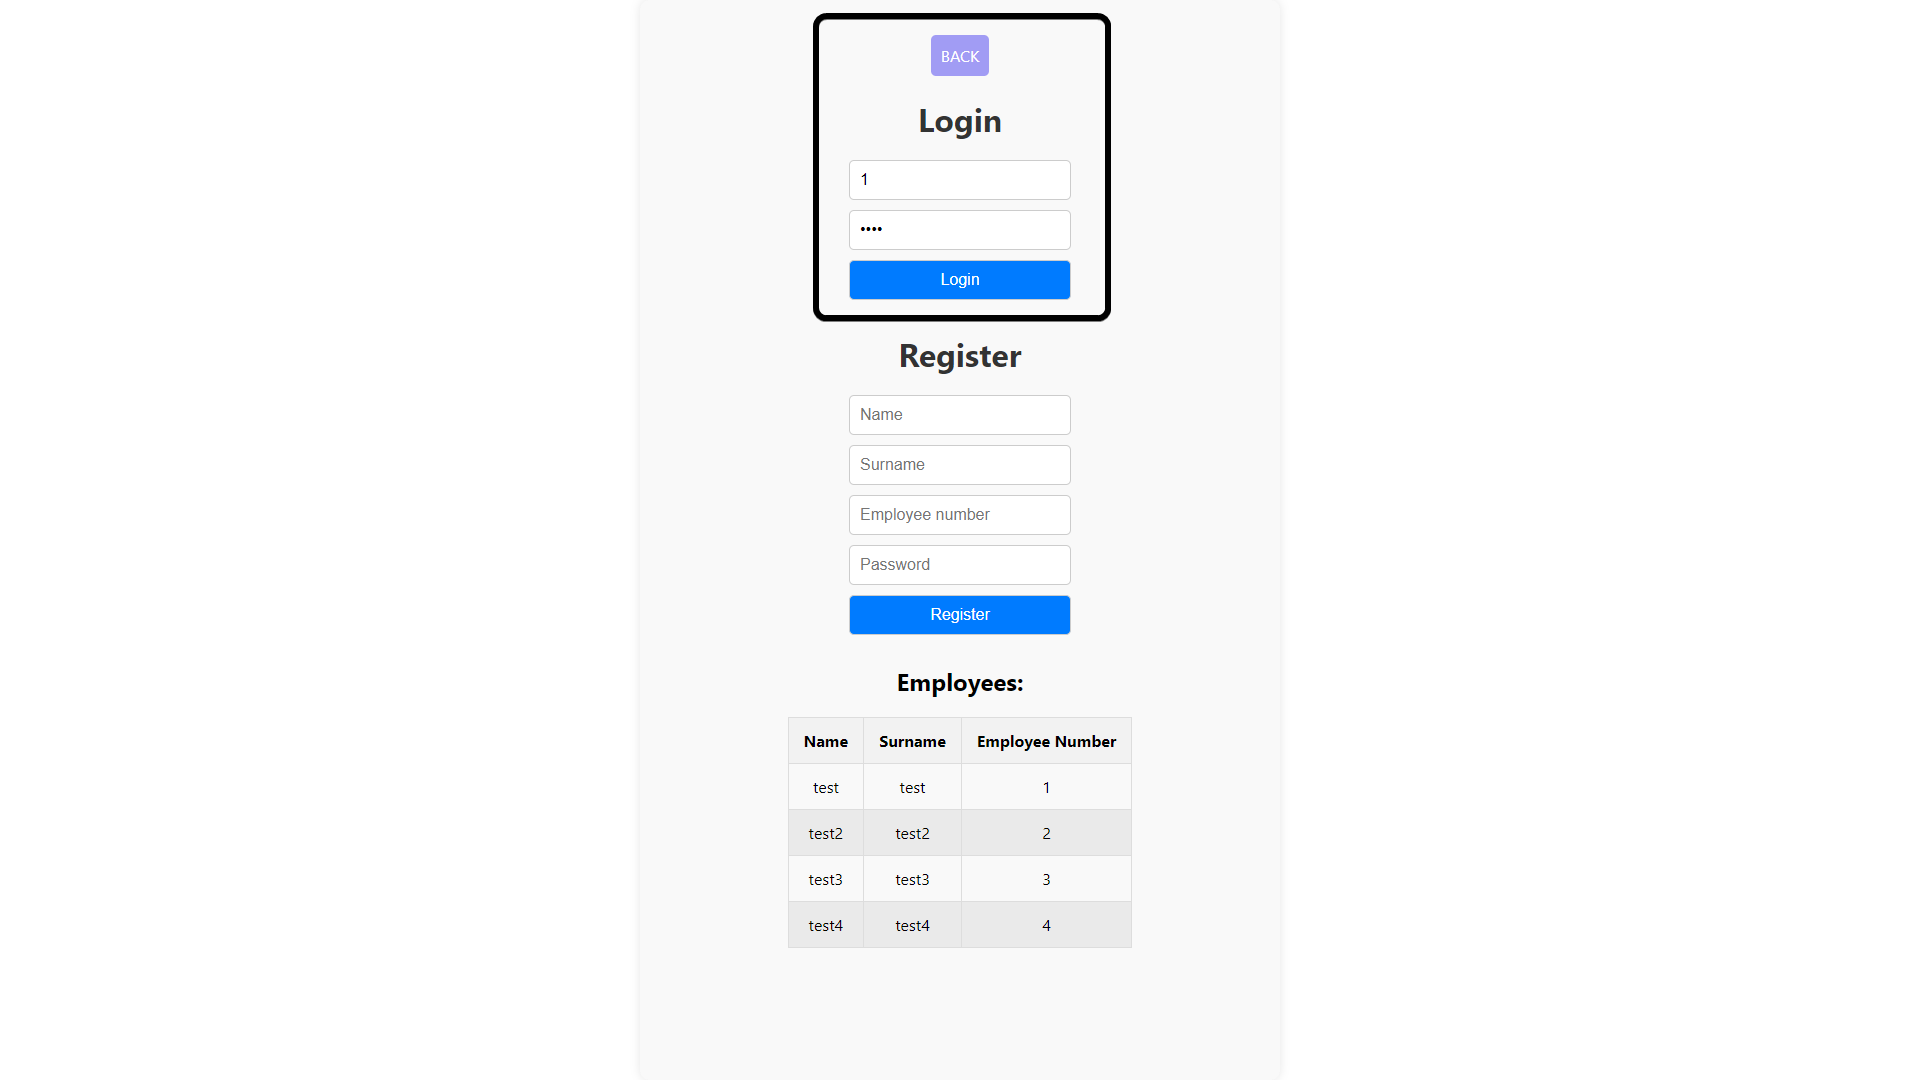
\includegraphics[width=\textwidth]{media/Login_login.png}
\end{center}
\end{minipage}

\begin{minipage}{\textwidth}
\noindent Po podaniu poprawnych danych, zostajemy zalogowani:
\begin{center}
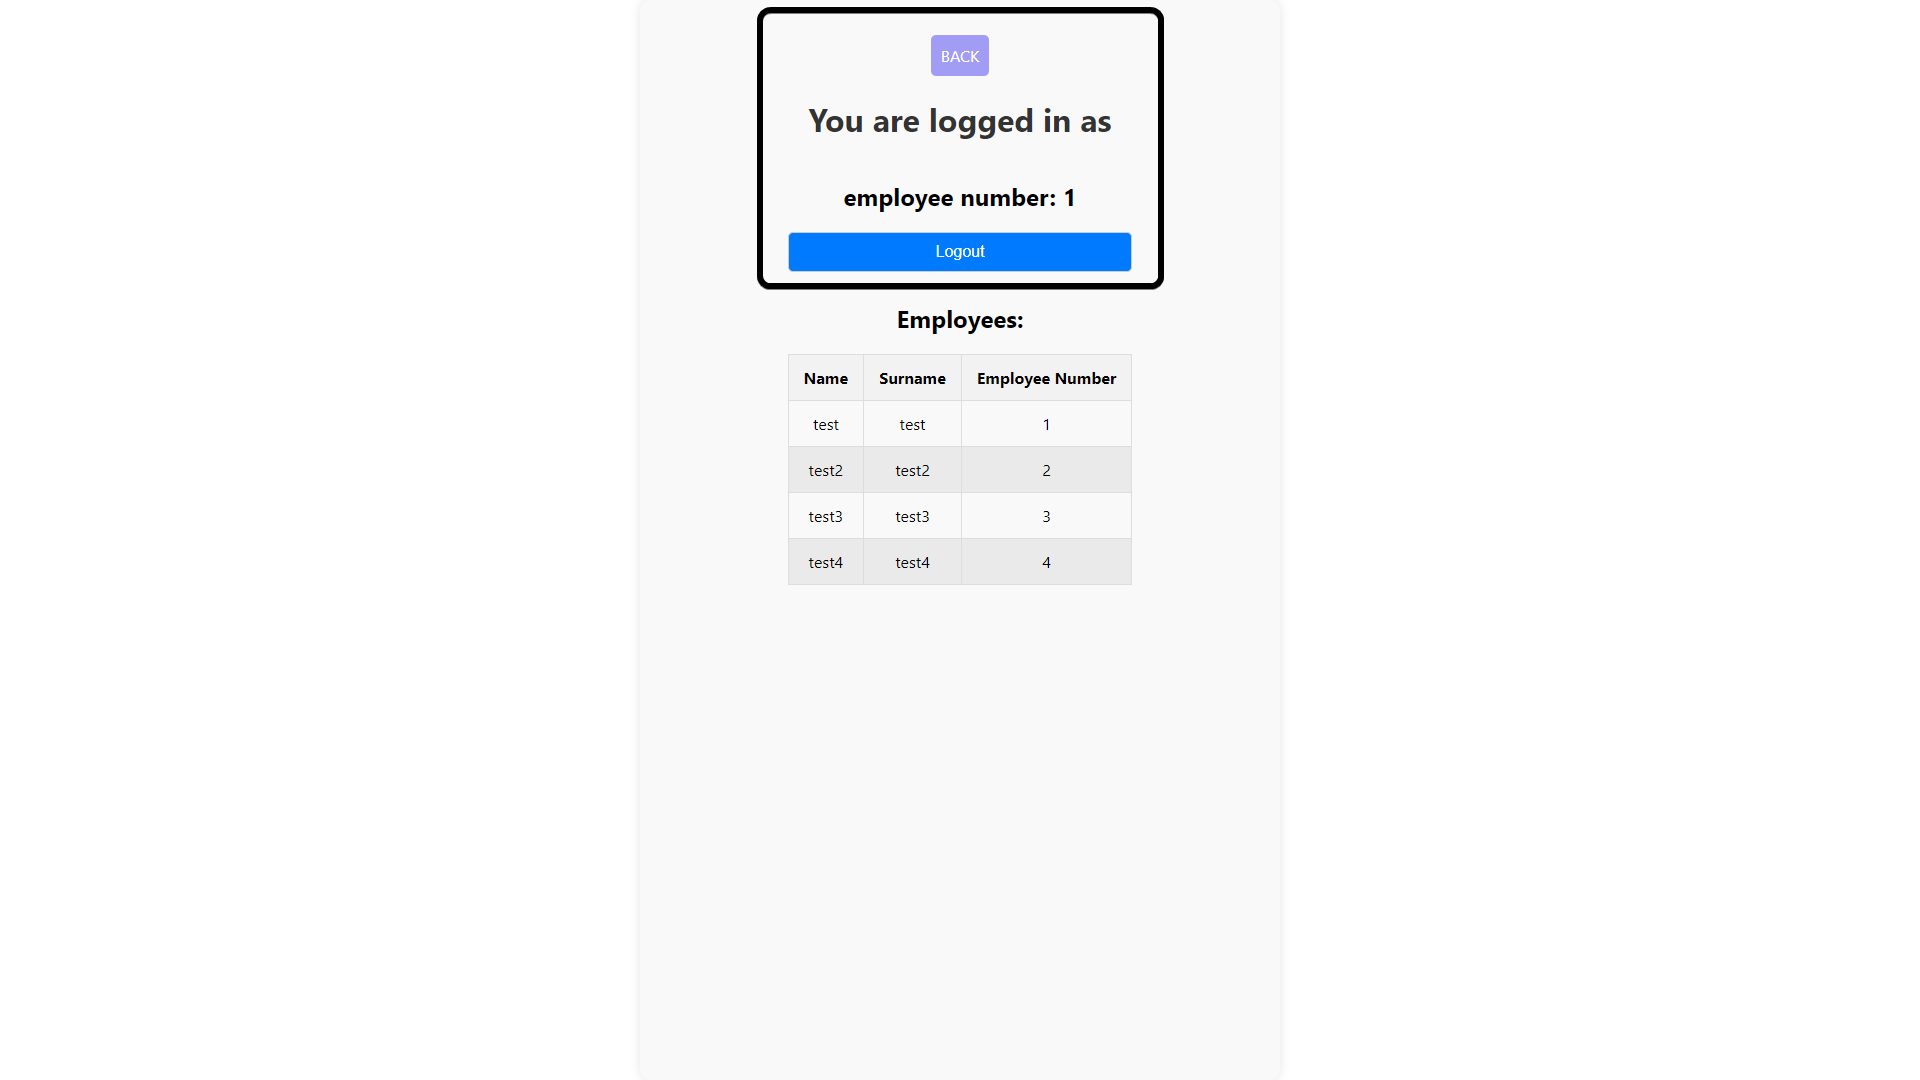
\includegraphics[width=\textwidth]{media/Login_successfull.png}
\end{center}
\end{minipage}

\begin{minipage}{\textwidth}
\noindent Jeśli podamy złe dane logowania, dostajemy komunikat:
\begin{center}
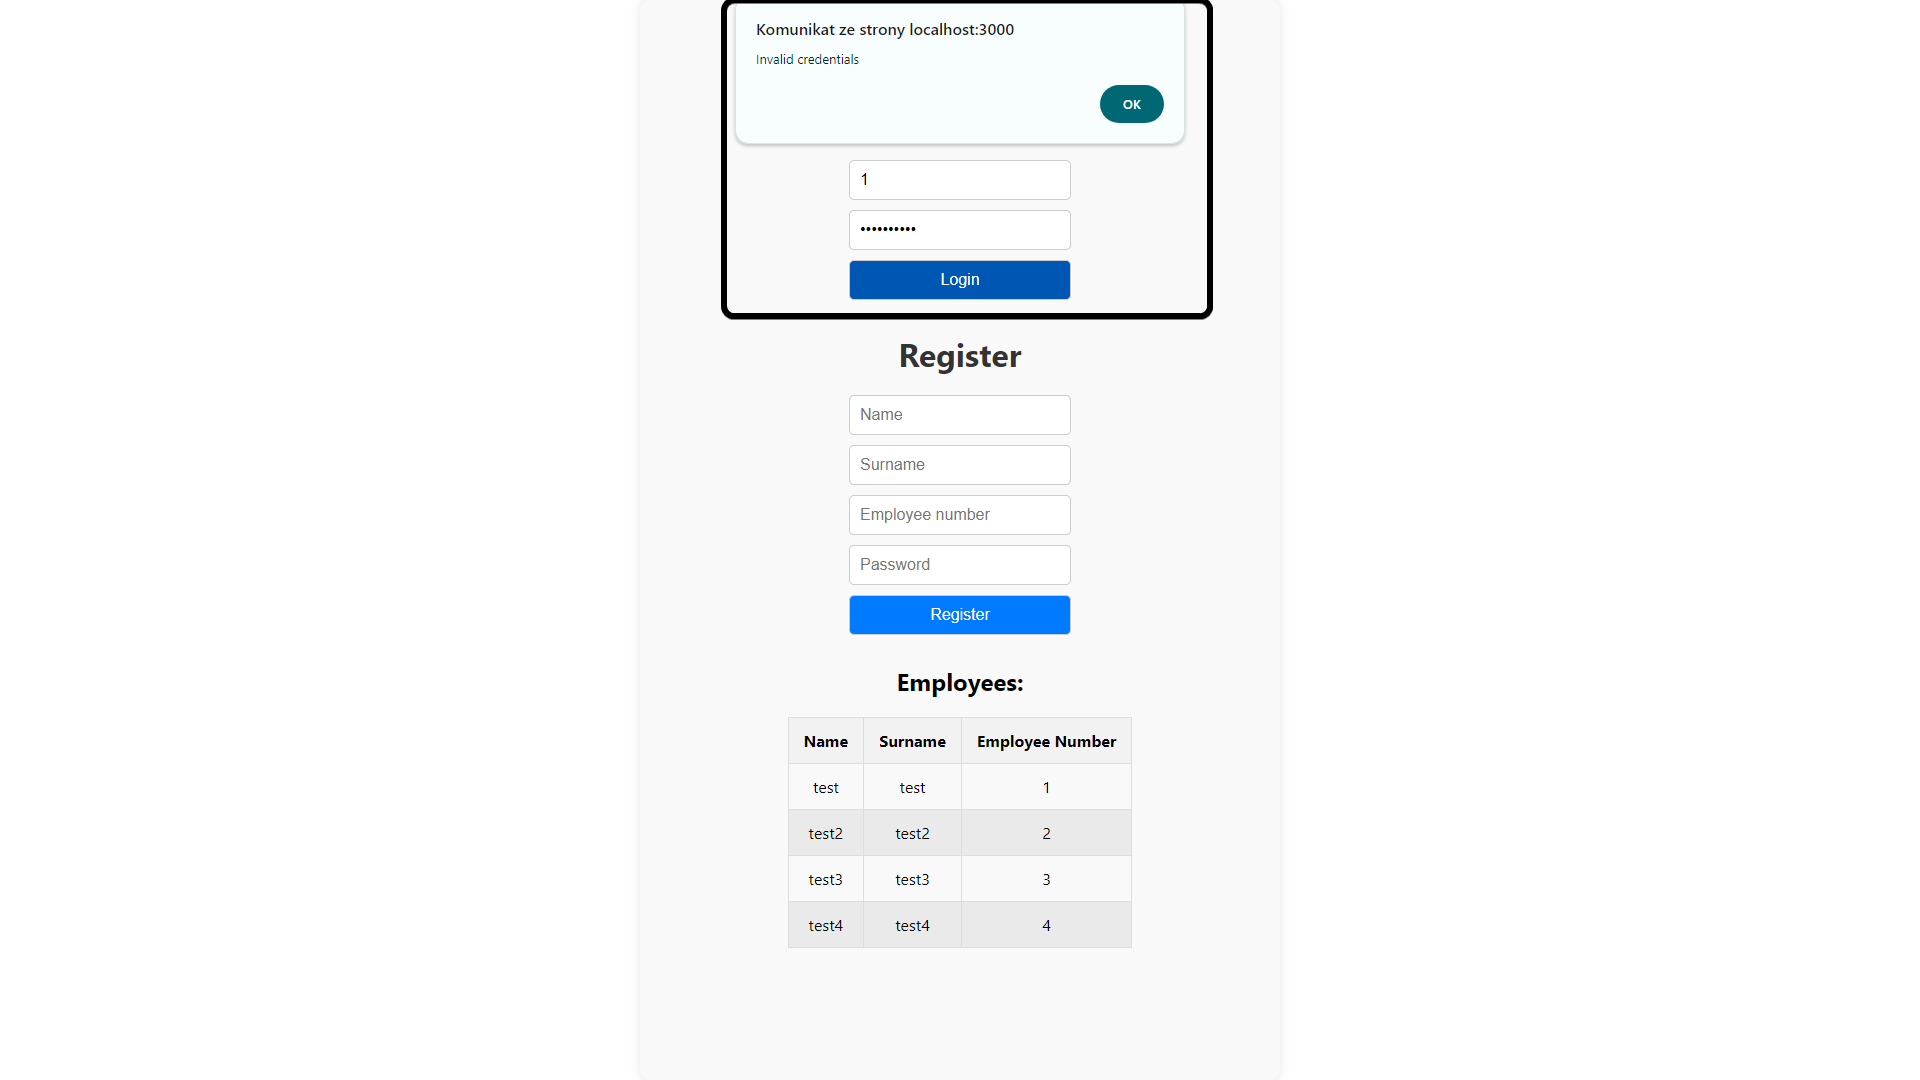
\includegraphics[width=\textwidth]{media/Login_invalidCredentials.png}
\end{center}
\end{minipage}

\begin{minipage}{\textwidth}
\noindent Możemy również zarejestrować nowego pracownika:
\begin{center}
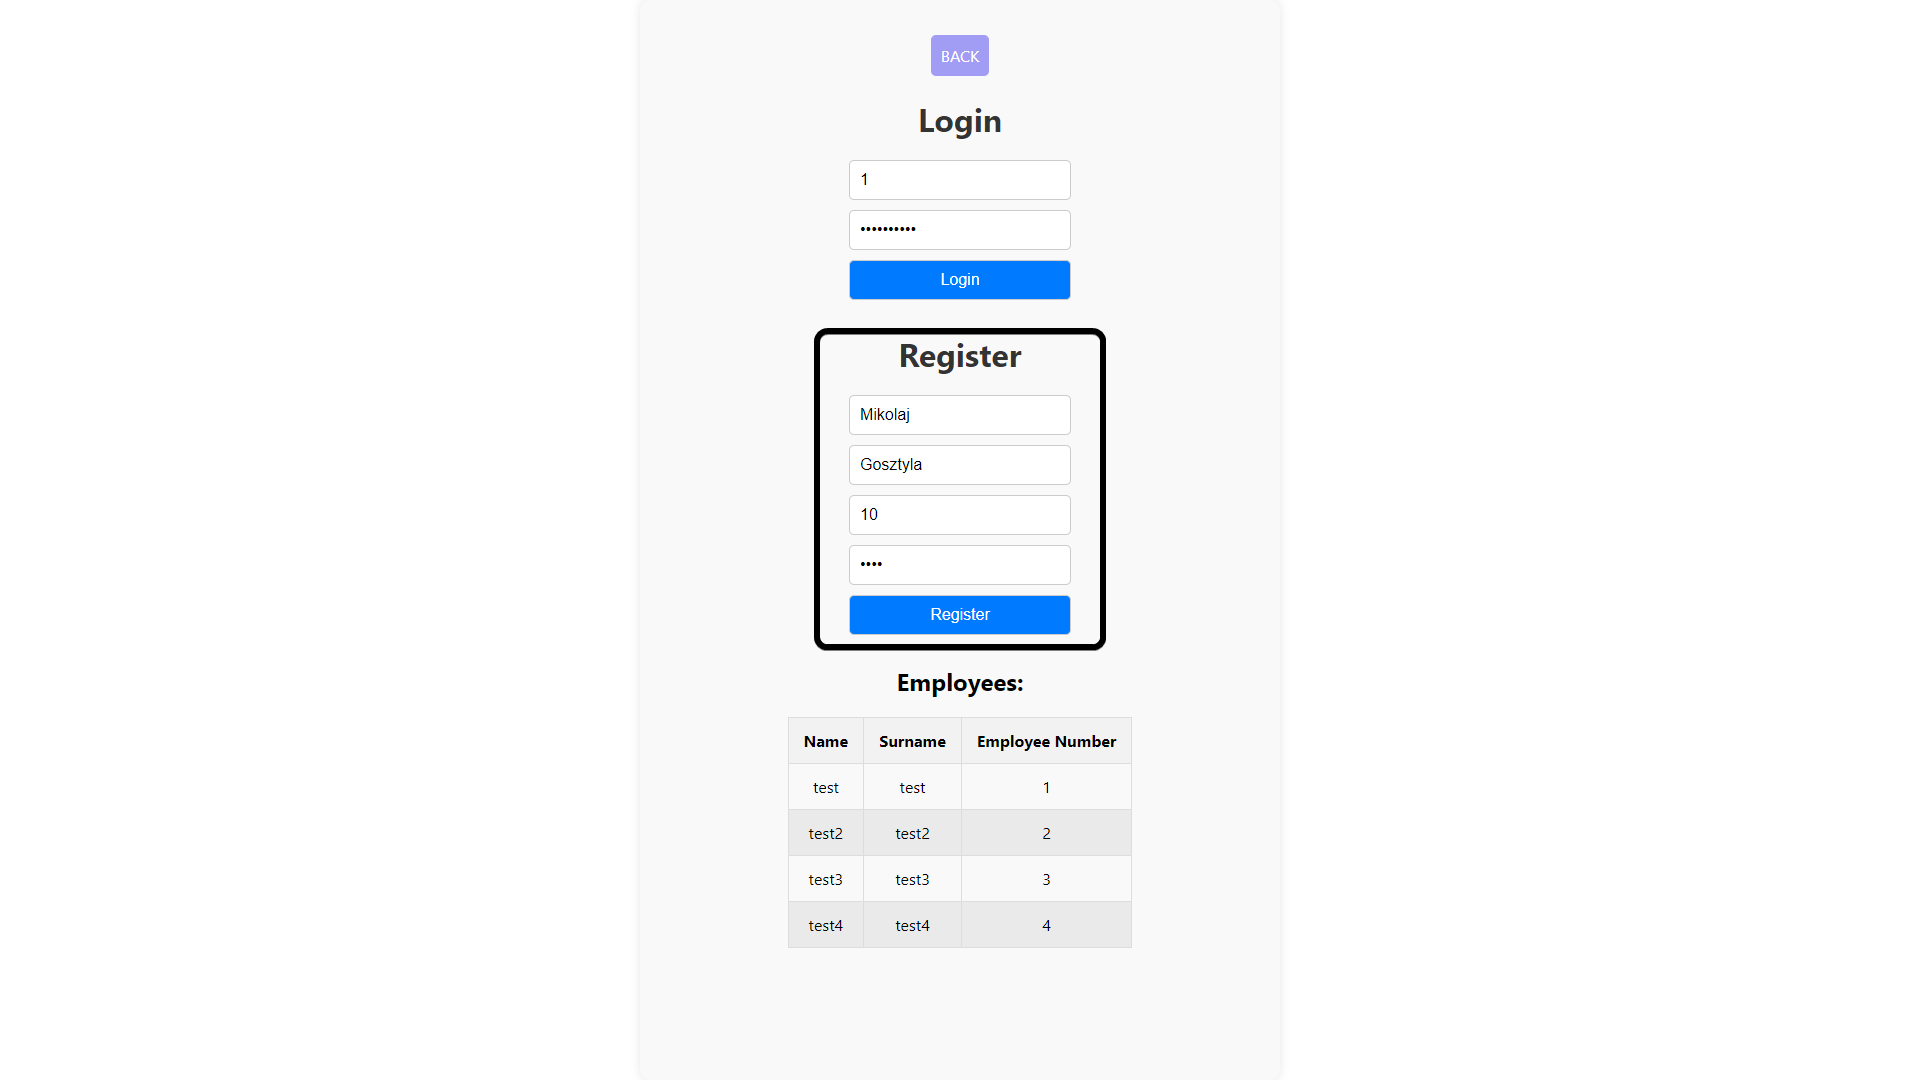
\includegraphics[width=\textwidth]{media/Login_register.png}
\end{center}
\end{minipage}

\begin{minipage}{\textwidth}
\noindent Po podaniu poprawnych danych, pracownik zostaje dodany do listy wszystkich zarejestrowanych pracowników:
\begin{center}
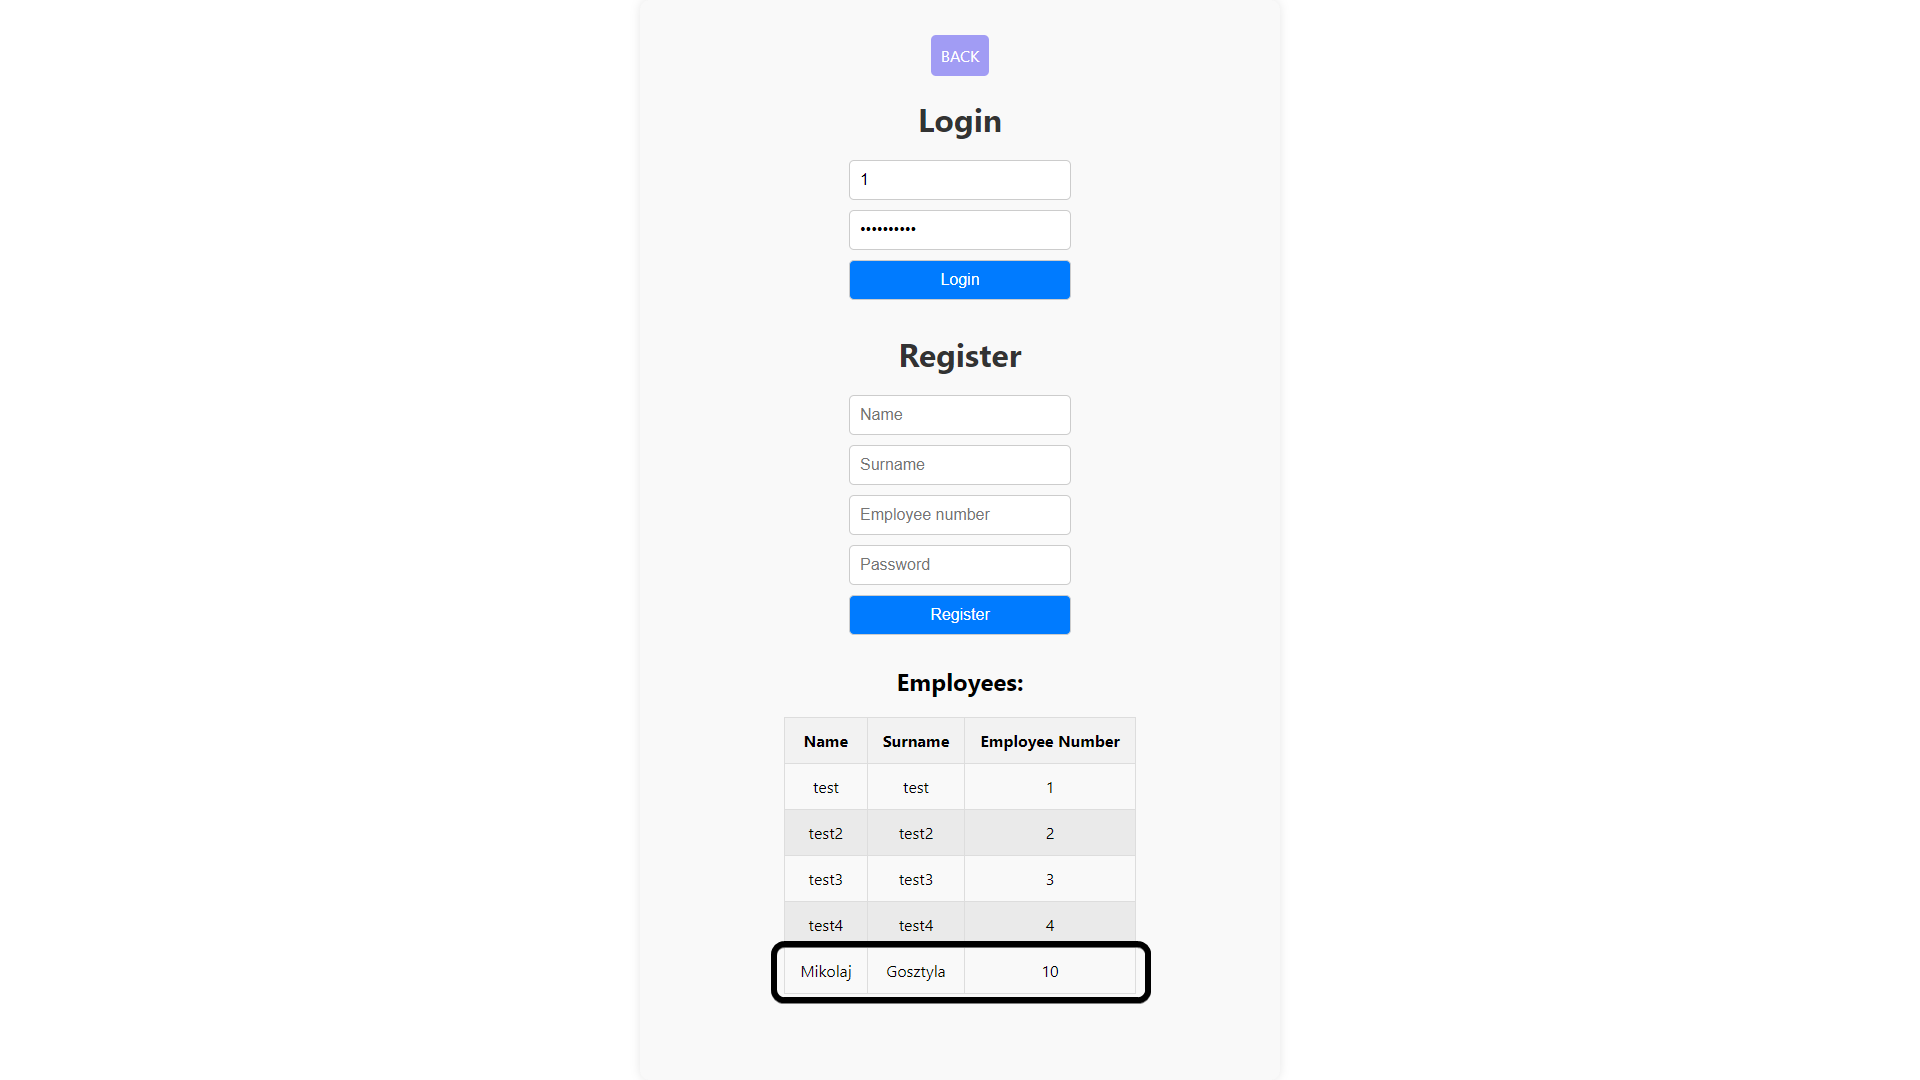
\includegraphics[width=\textwidth]{media/Login_registrationSuccessfull.png}
\end{center}
\end{minipage}

\begin{minipage}{\textwidth}
\noindent W przypadku, gdy dane nie są poprawne, dostajemy komunikat:
\begin{center}
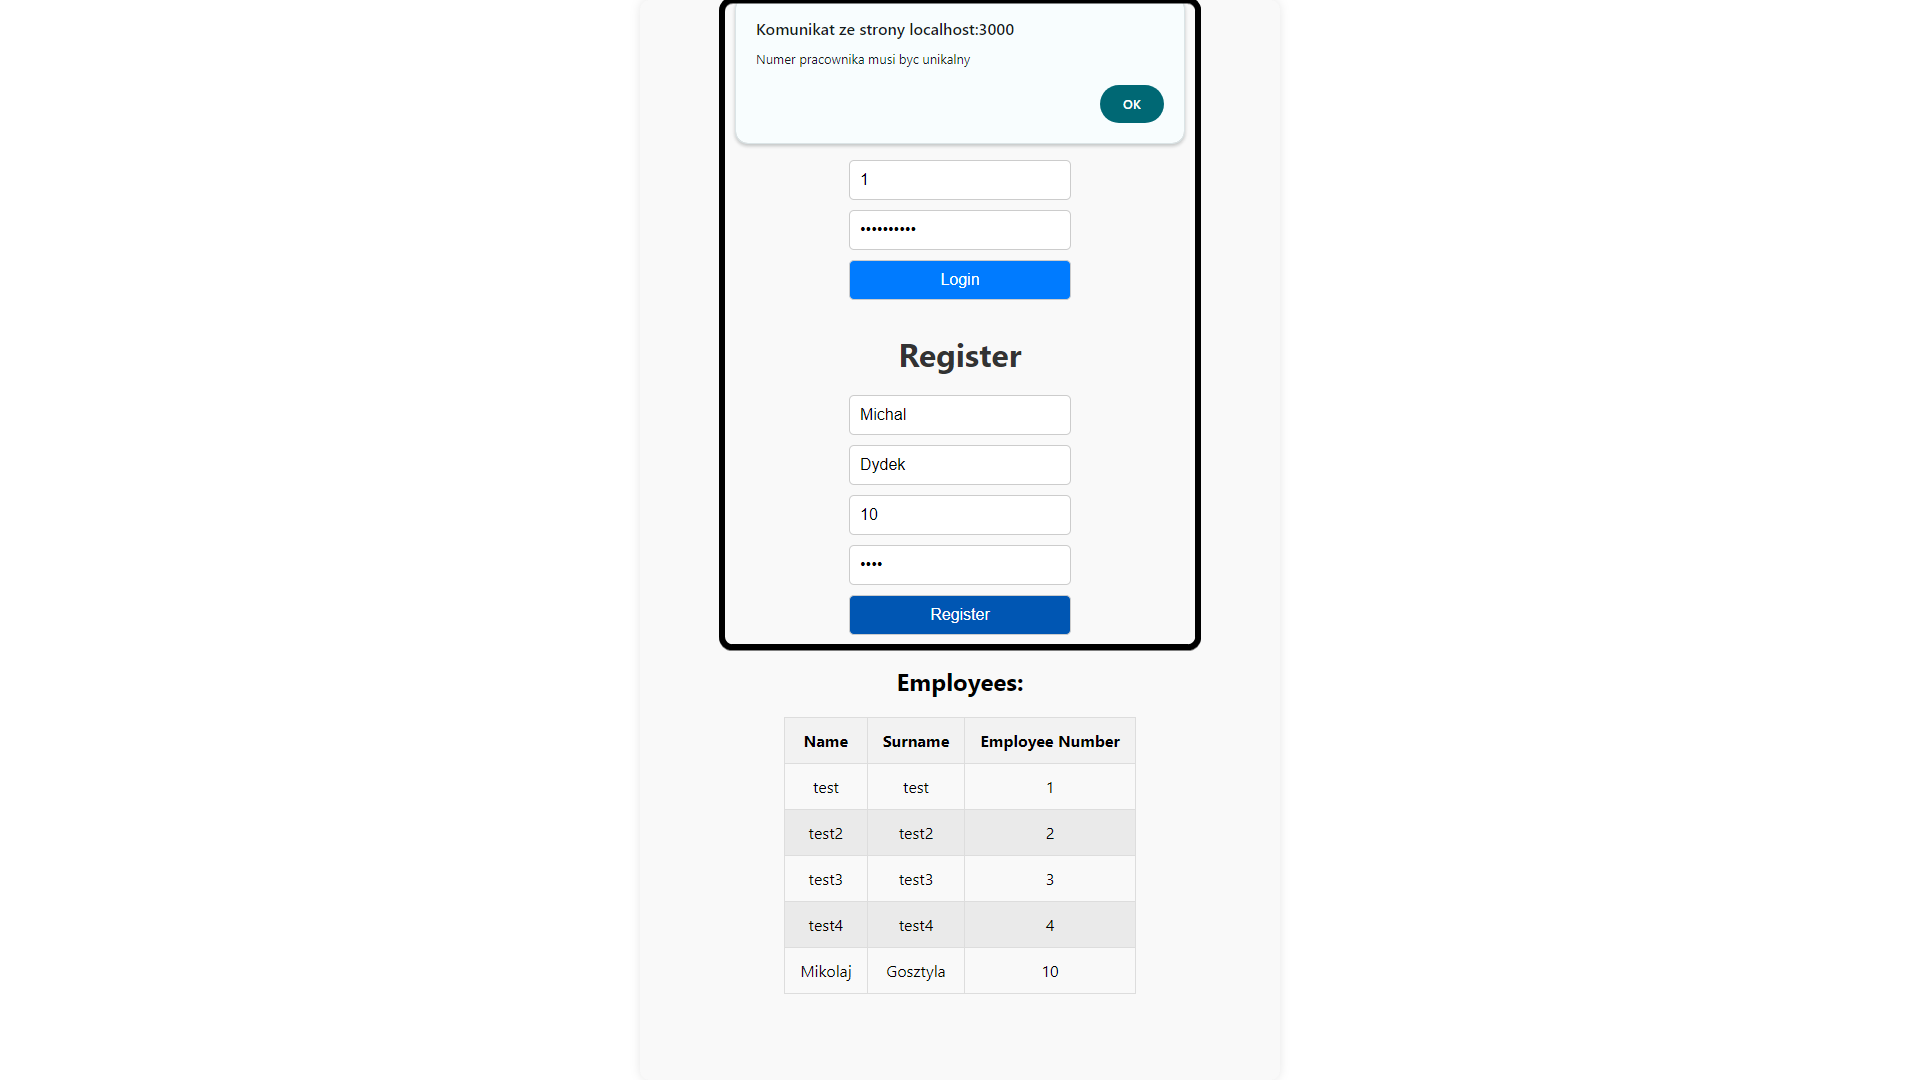
\includegraphics[width=\textwidth]{media/Login_uniqueNumber.png}
\end{center}
\end{minipage}

\newpage
\subsection{Expenses}
\begin{minipage}{\textwidth}
\noindent Po wciśnięciu przycisku \textbf{Expenses}:
\begin{center}
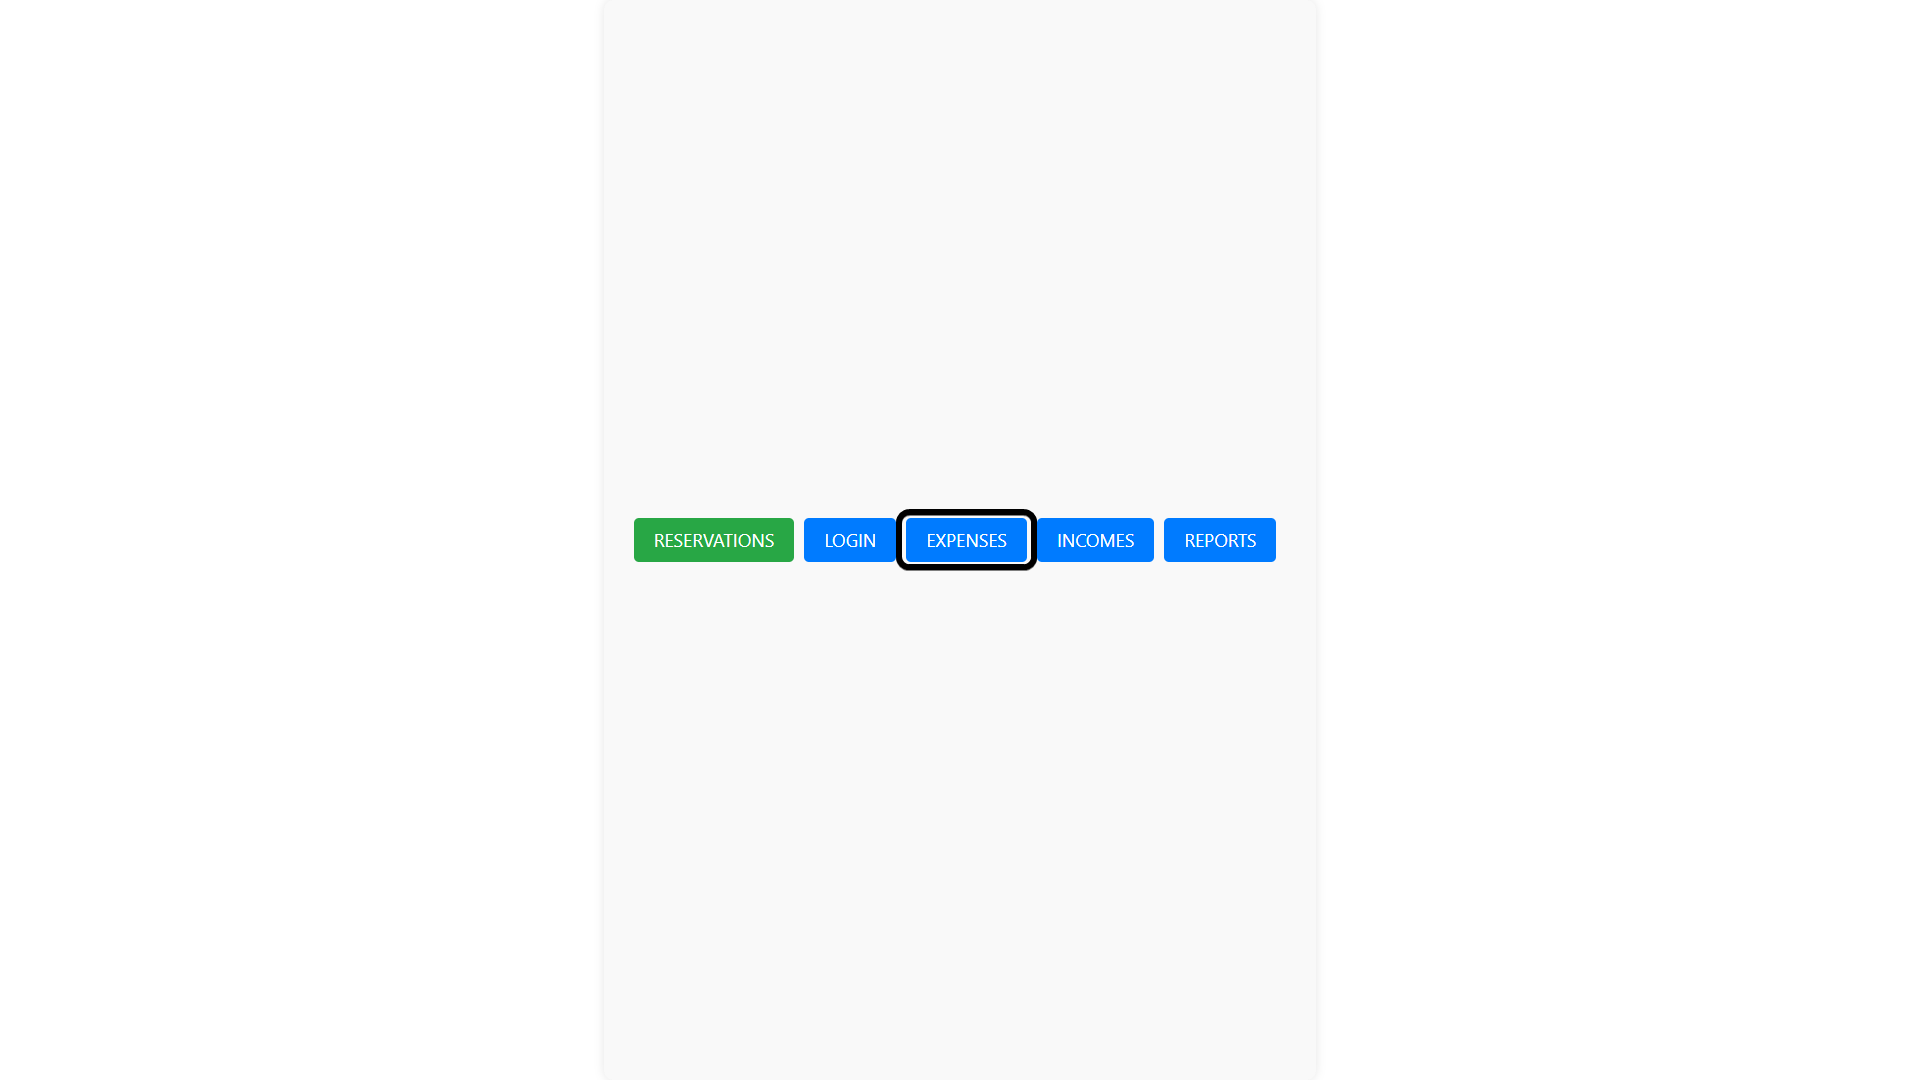
\includegraphics[width=\textwidth]{media/Expenses.png}
\end{center}
\end{minipage}

\begin{minipage}{\textwidth}
\noindent Przenosimy się do panelu wydatków:
\begin{center}
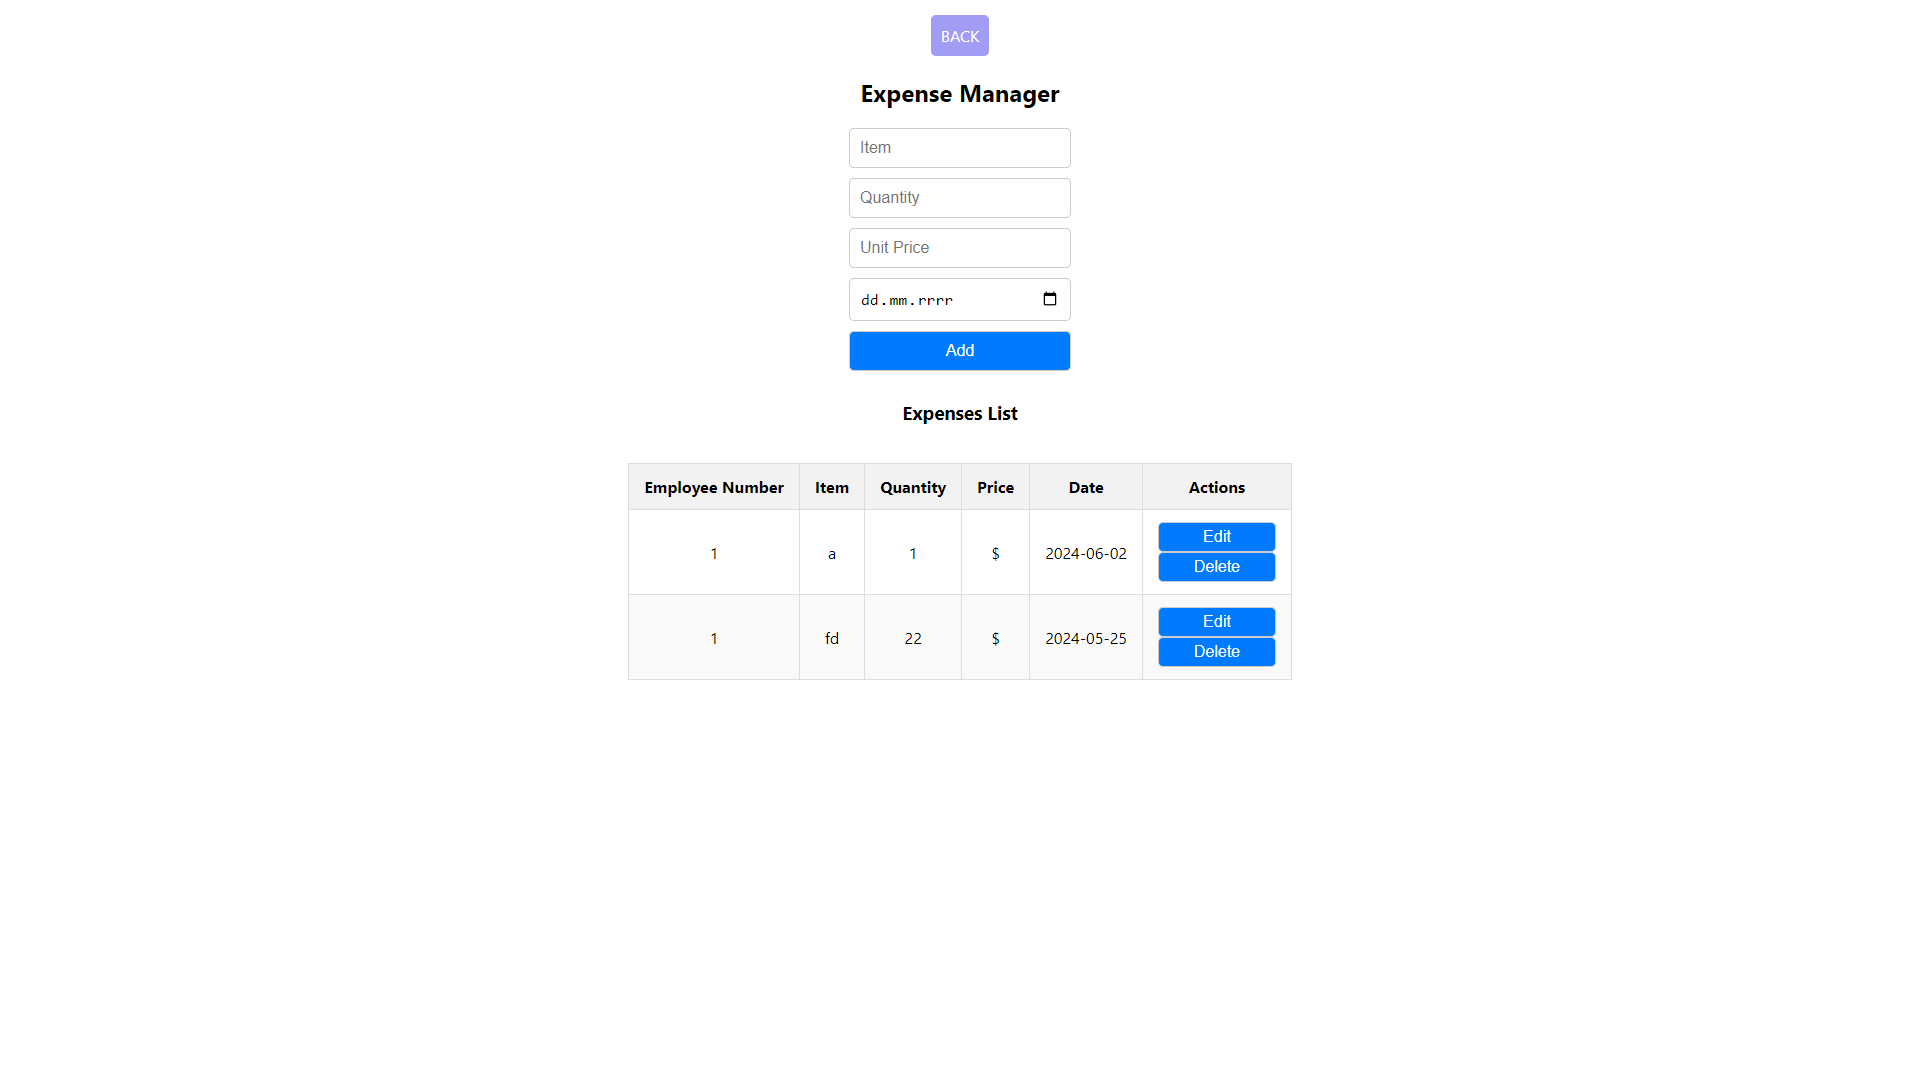
\includegraphics[width=\textwidth]{media/Expenses_in.png}
\end{center}
\end{minipage}

\begin{minipage}{\textwidth}
\noindent Mamy możliwość dodana nowego wydatku:
\begin{center}
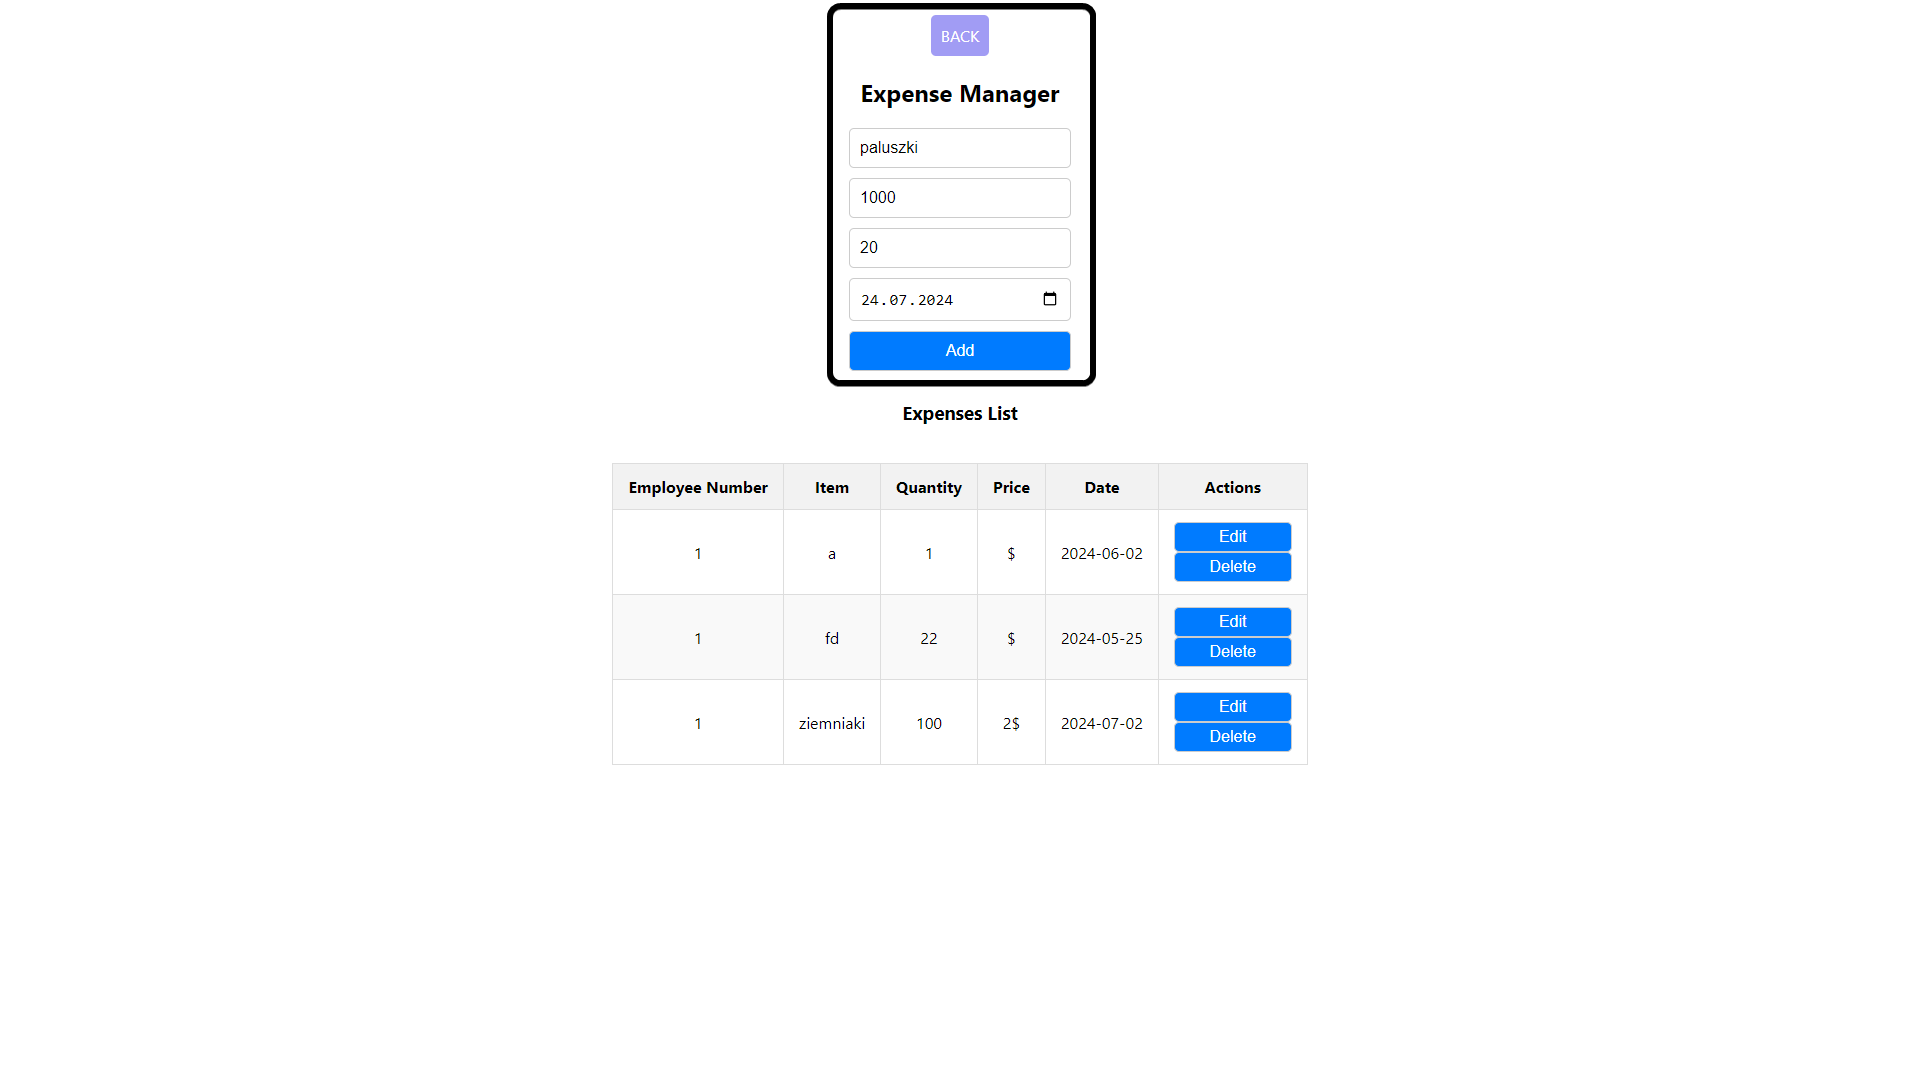
\includegraphics[width=\textwidth]{media/Expenses_input.png}
\end{center}
\end{minipage}

\begin{minipage}{\textwidth}
\noindent Po wciśniąciu przycisku \textbf{Add}, wydatek zostaje dodany do listy:
\begin{center}
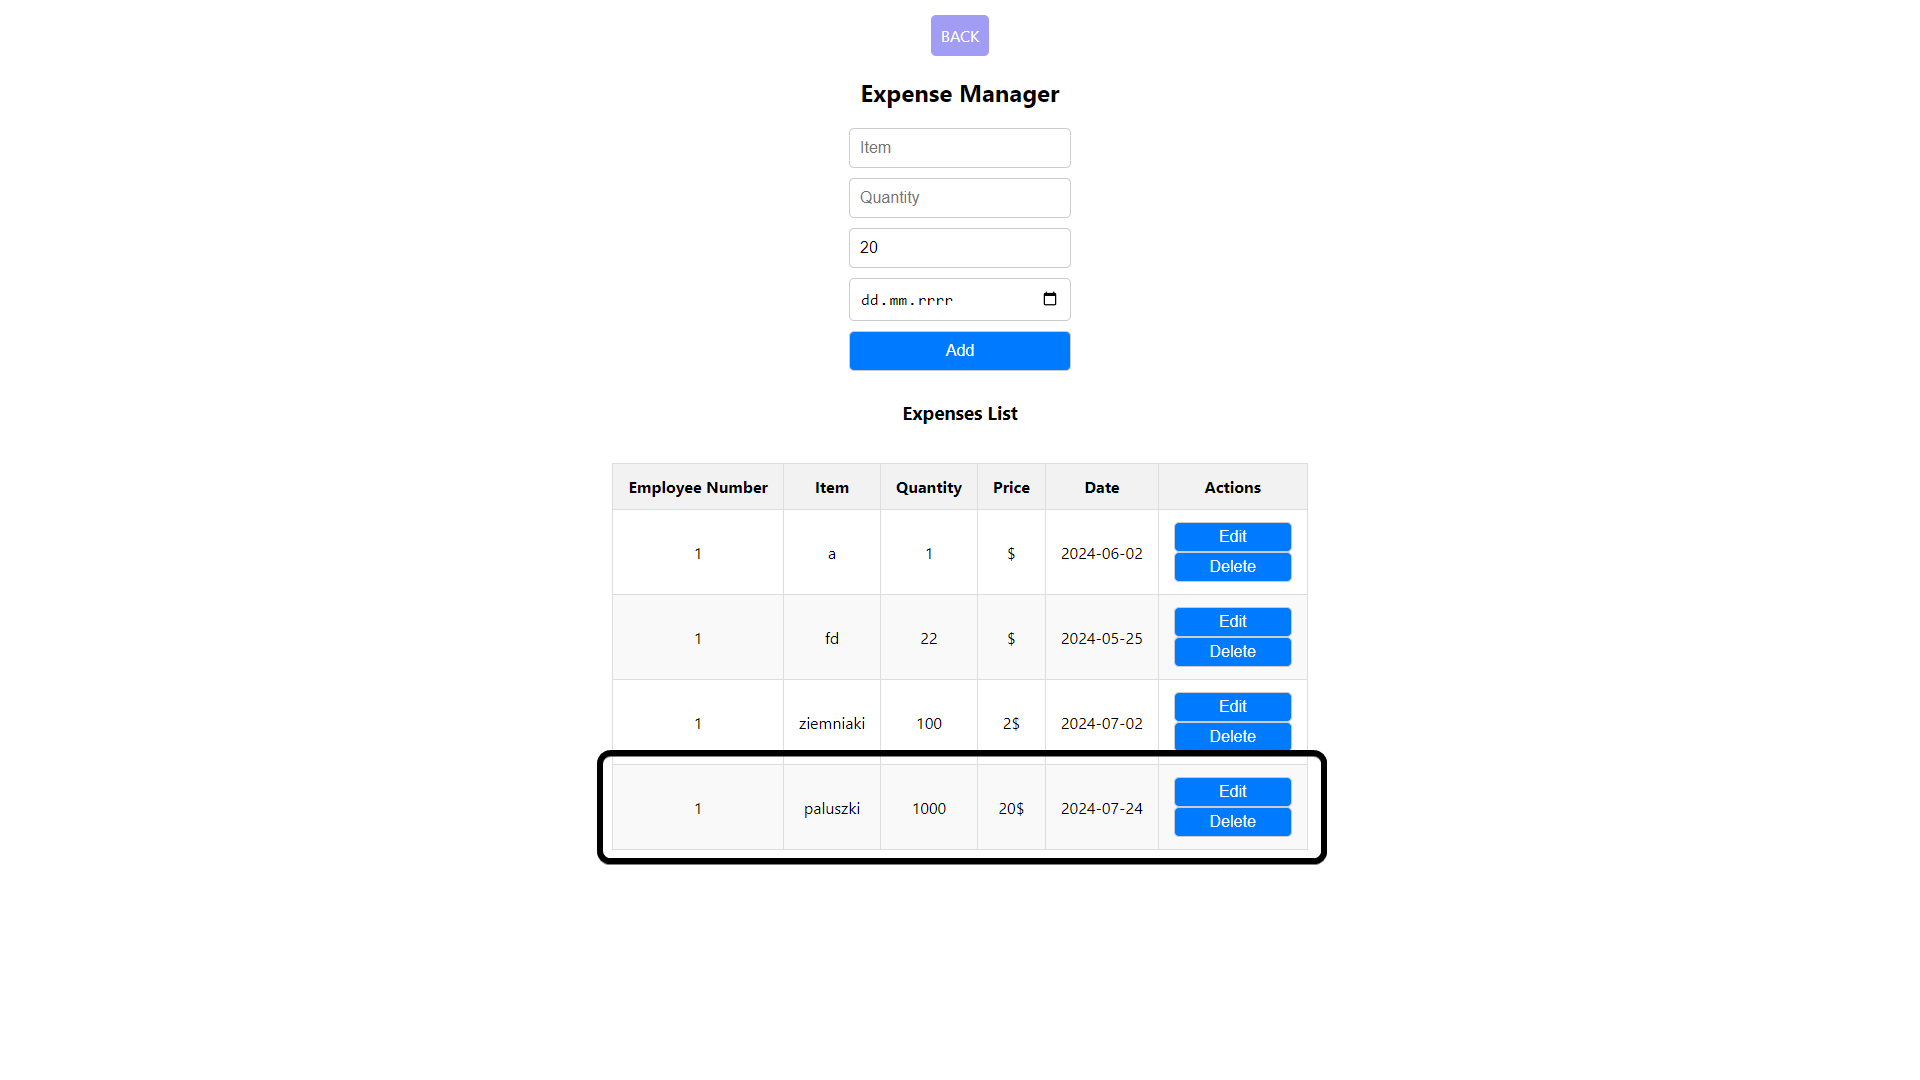
\includegraphics[width=\textwidth]{media/Expenses_add.png}
\end{center}
\end{minipage}

\begin{minipage}{\textwidth}
\noindent Mamy możliwość edycji dodanego wcześniej wydatku:
\begin{center}
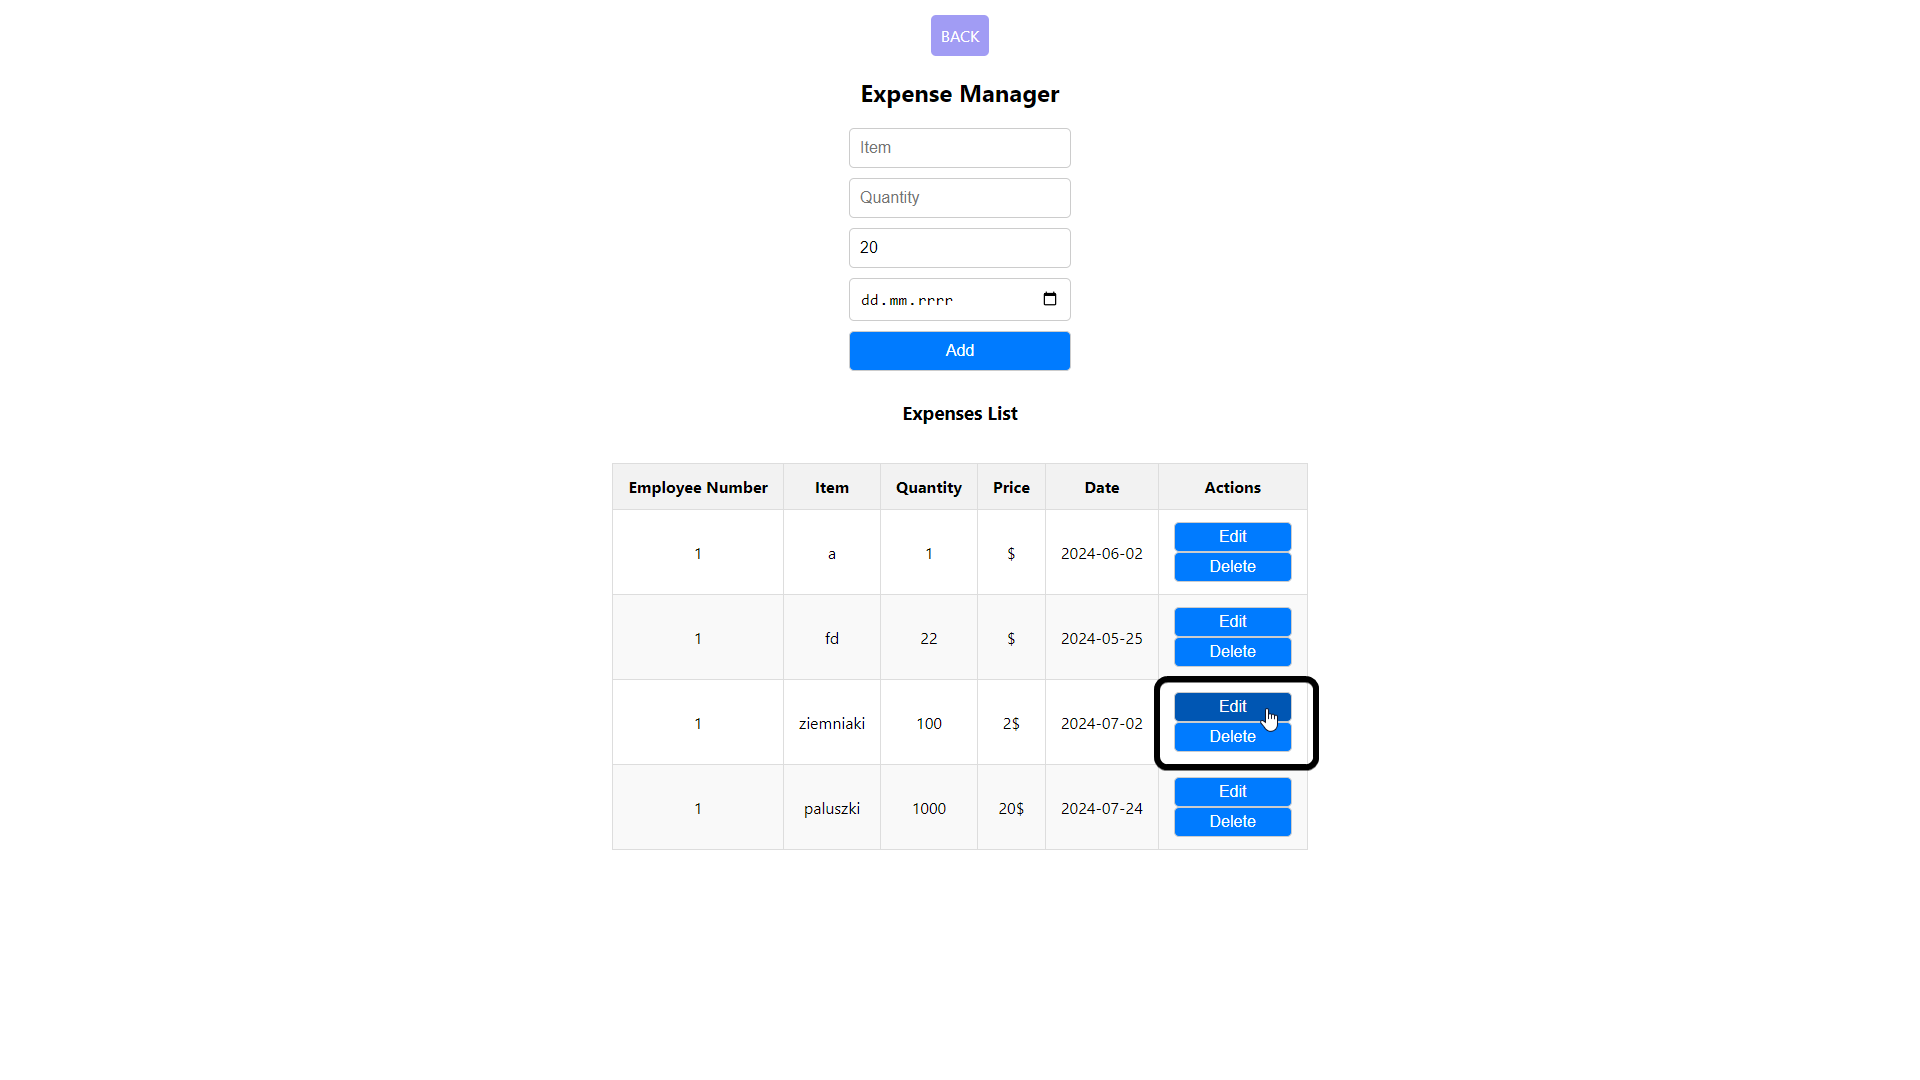
\includegraphics[width=\textwidth]{media/Expenses_edit.png}
\end{center}
\end{minipage}

\begin{minipage}{\textwidth}
\noindent Po wciśnięciu przycisku \textbf{Edit}, dane o wybranych wydatku zostają automatycznie uzupełnione w panelu na górze:
\begin{center}
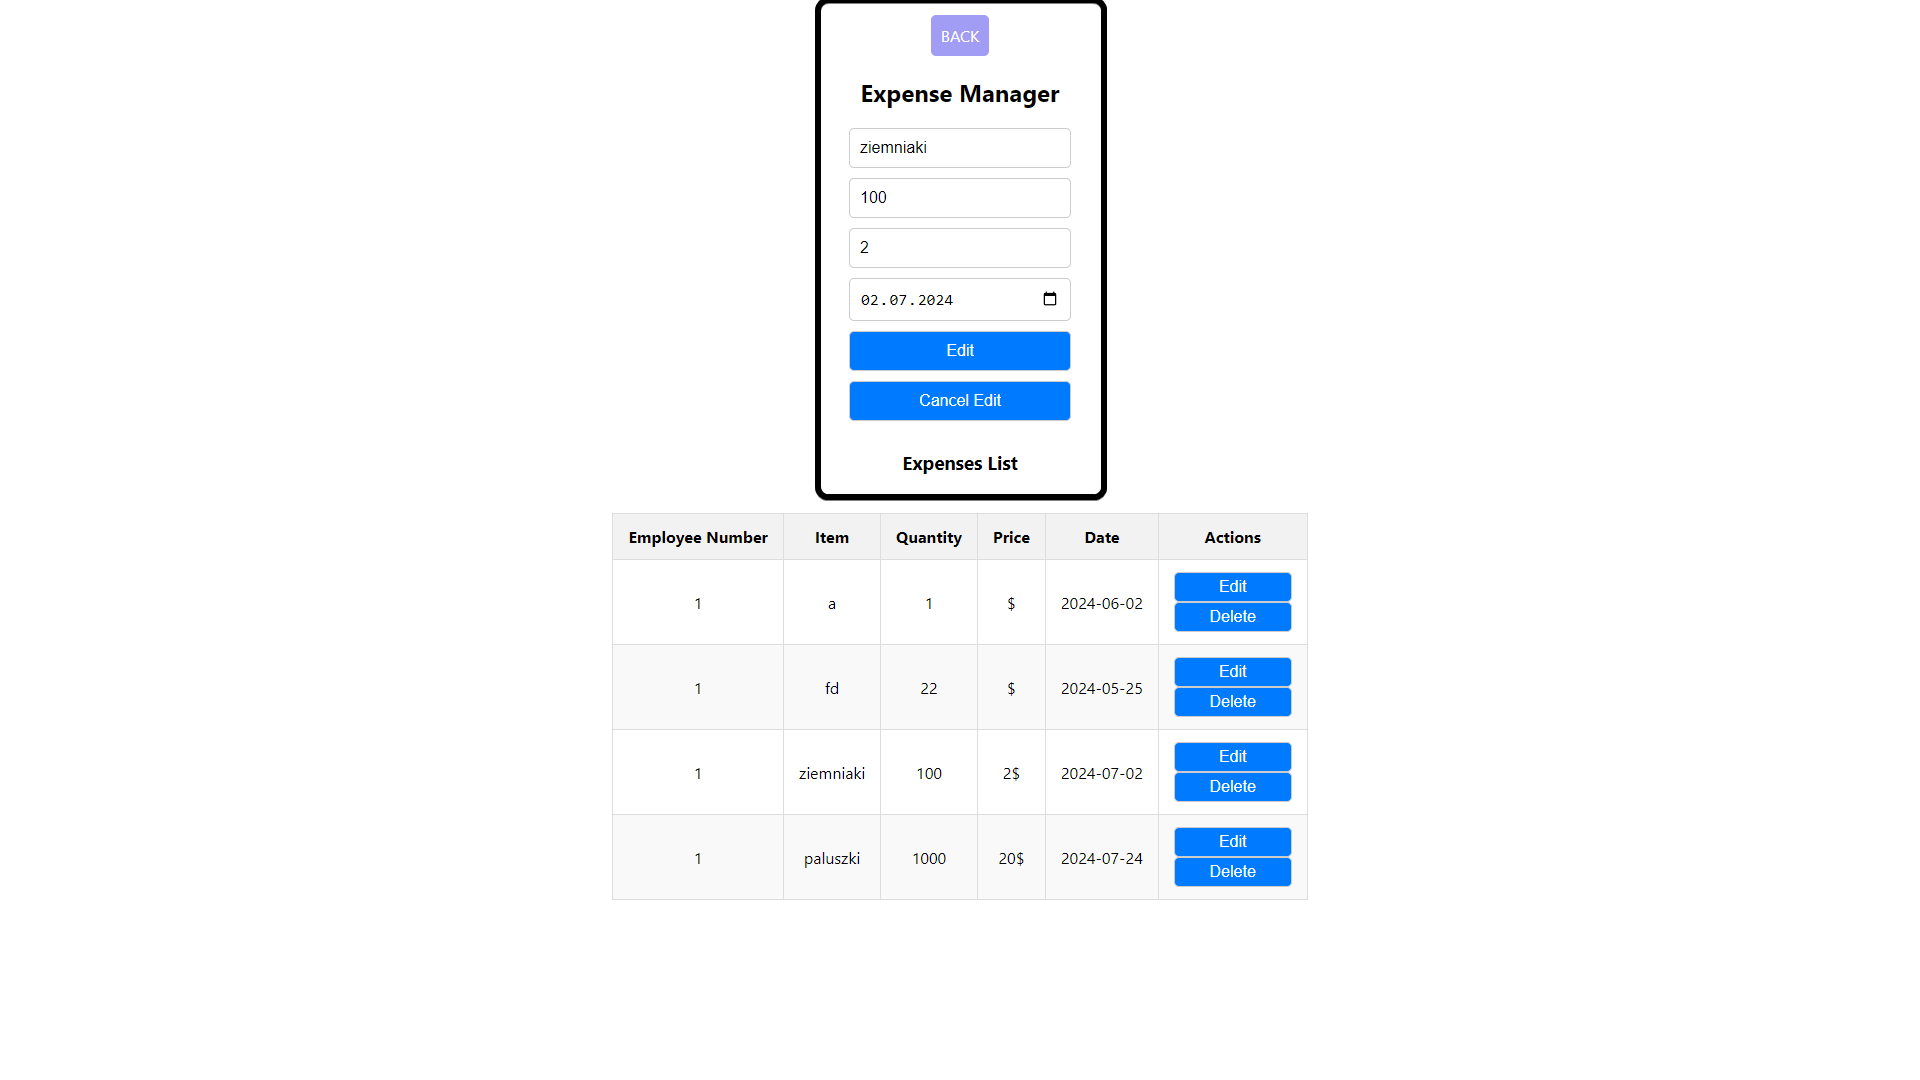
\includegraphics[width=\textwidth]{media/Expenses_editValues.png}
\end{center}
\end{minipage}

\begin{minipage}{\textwidth}
\noindent Mamy teraz możliwość edycji danych o wybranym wydatku:
\begin{center}
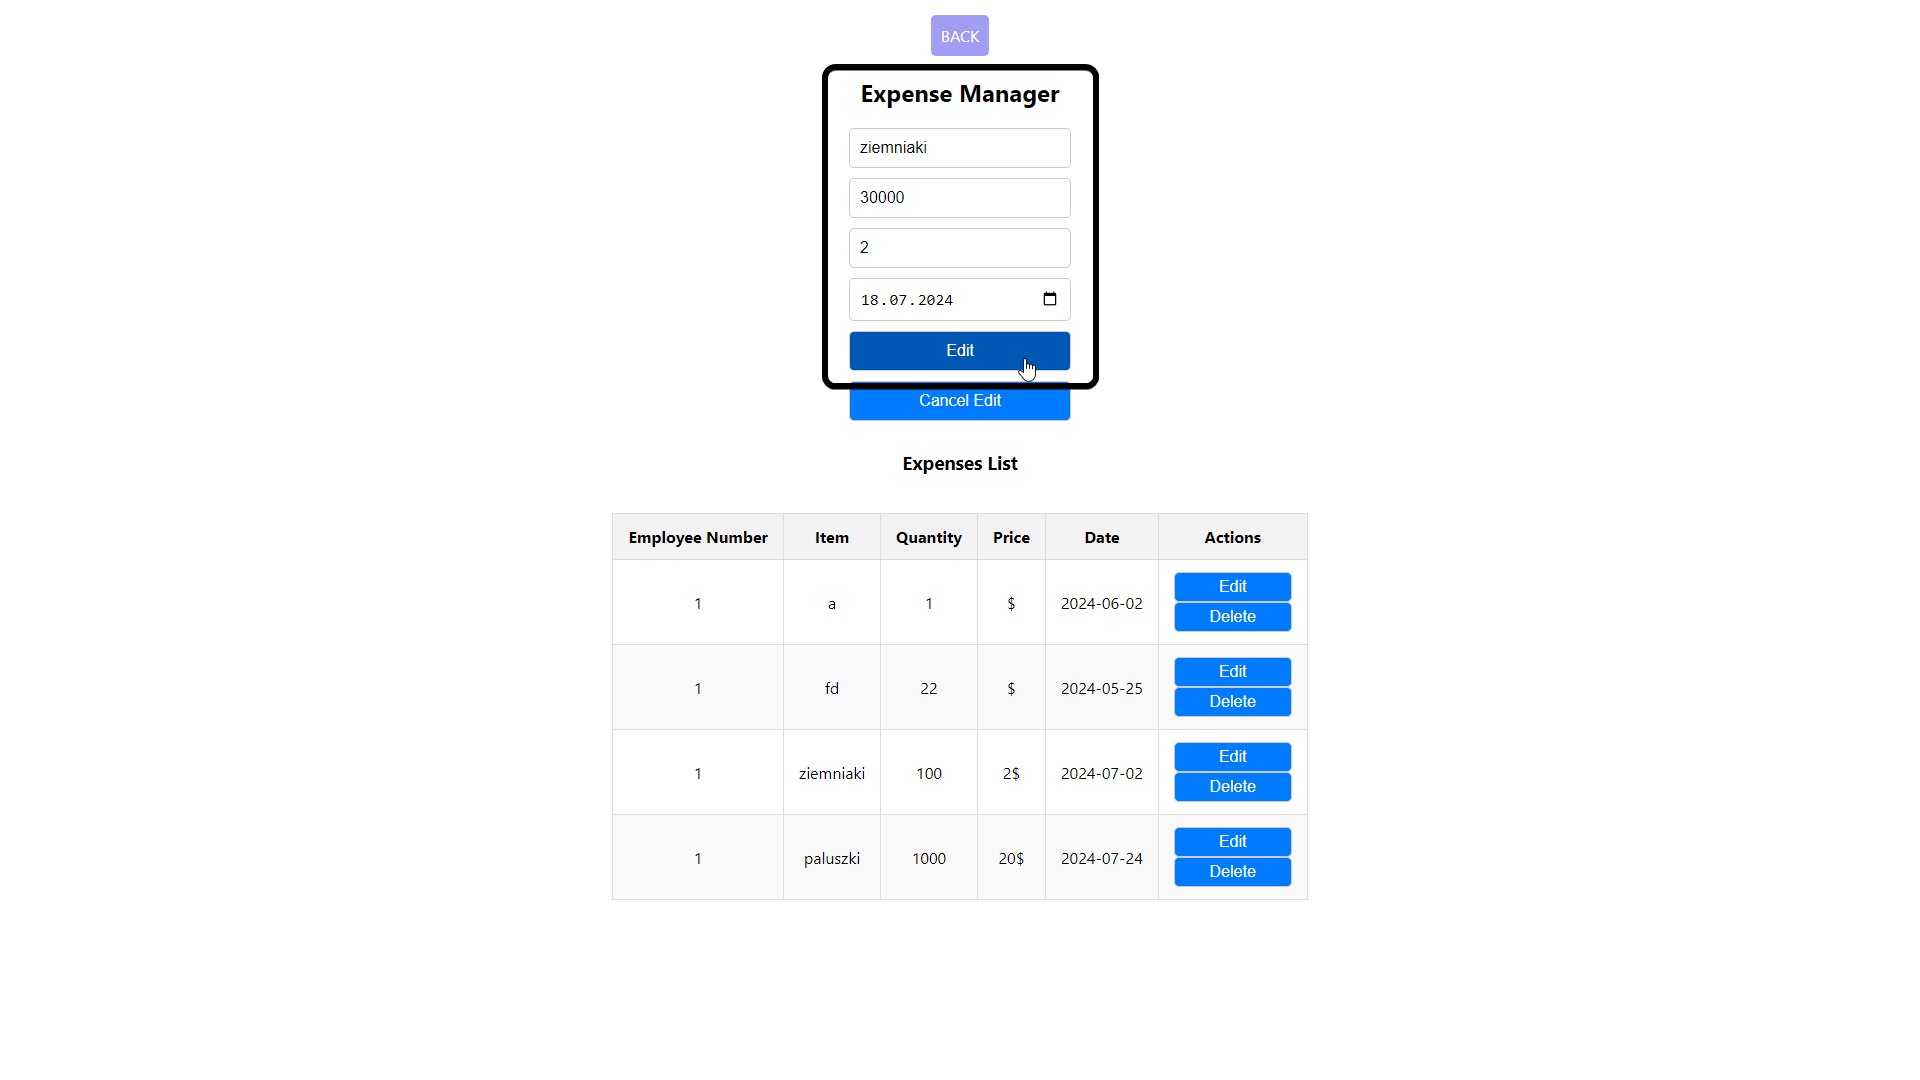
\includegraphics[width=\textwidth]{media/Expenses_newValues.png}
\end{center}
\end{minipage}

\begin{minipage}{\textwidth}
\noindent Po ponownym wciśnięciu przysku \textbf{Edit}, nowe dane zostają zapisane:
\begin{center}
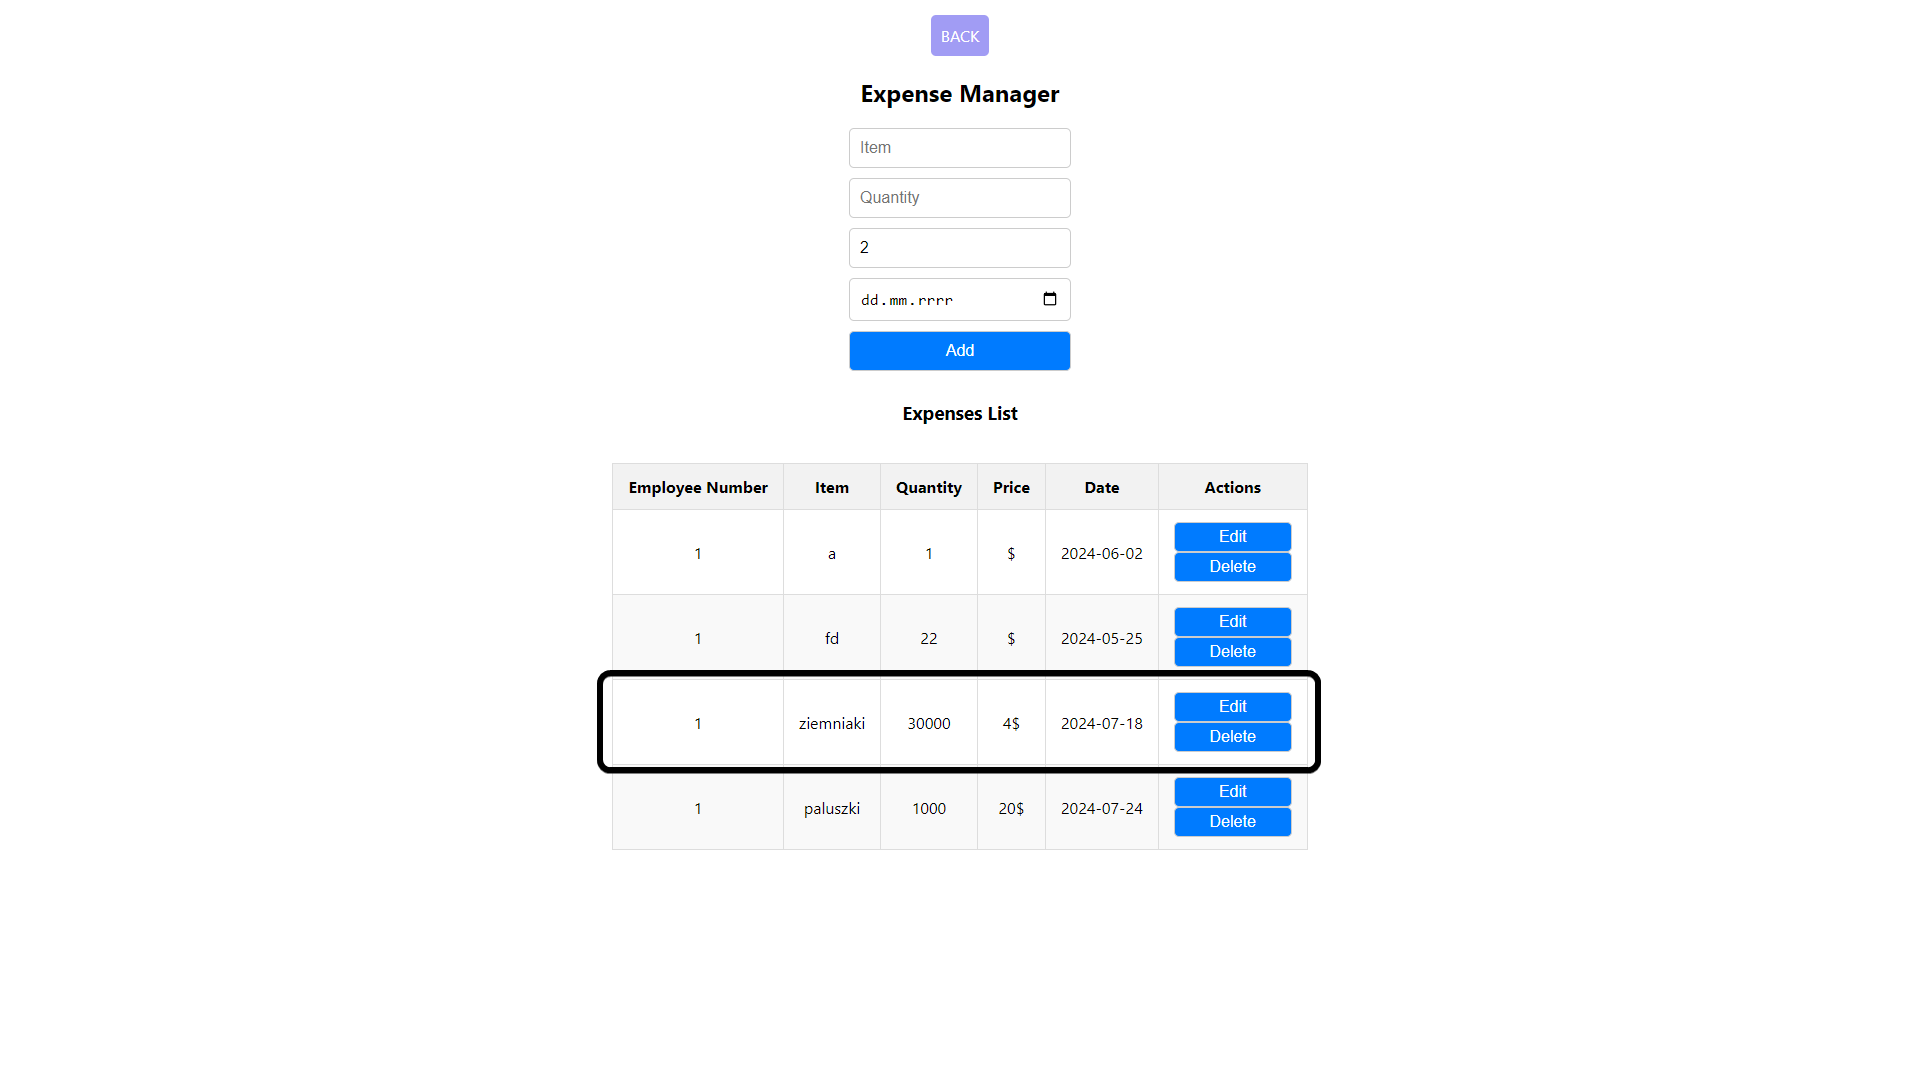
\includegraphics[width=\textwidth]{media/Expenses_editSuccessfull.png}
\end{center}
\end{minipage}

\begin{minipage}{\textwidth}
\noindent Jeśli jednak chcemy anulawać edycję danych o wybranym wydatku, możemy wcisnąć przycisk \textbf{Cancel Edit}:
\begin{center}
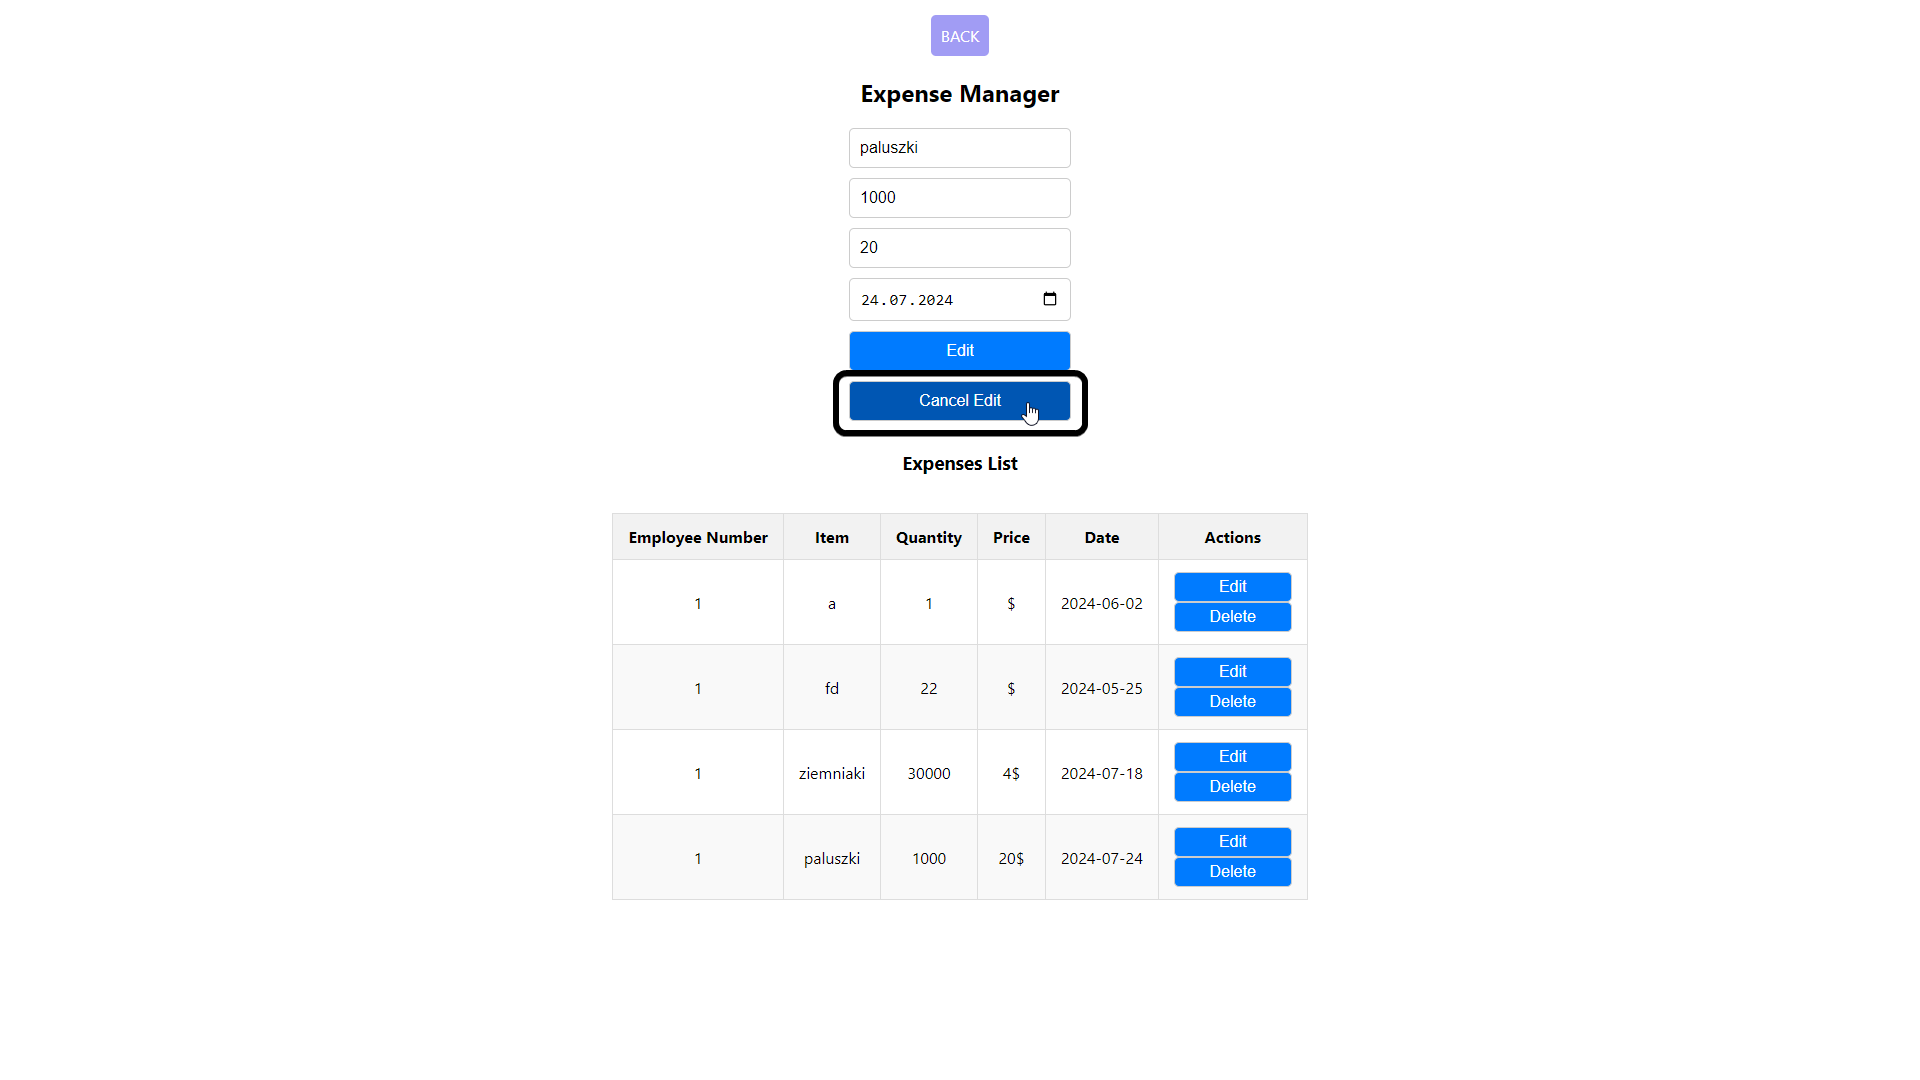
\includegraphics[width=\textwidth]{media/Expenses_cancelEdit.png}
\end{center}
\end{minipage}

\begin{minipage}{\textwidth}
\noindent Mamy również możliwość usunięcia wydatku:
\begin{center}
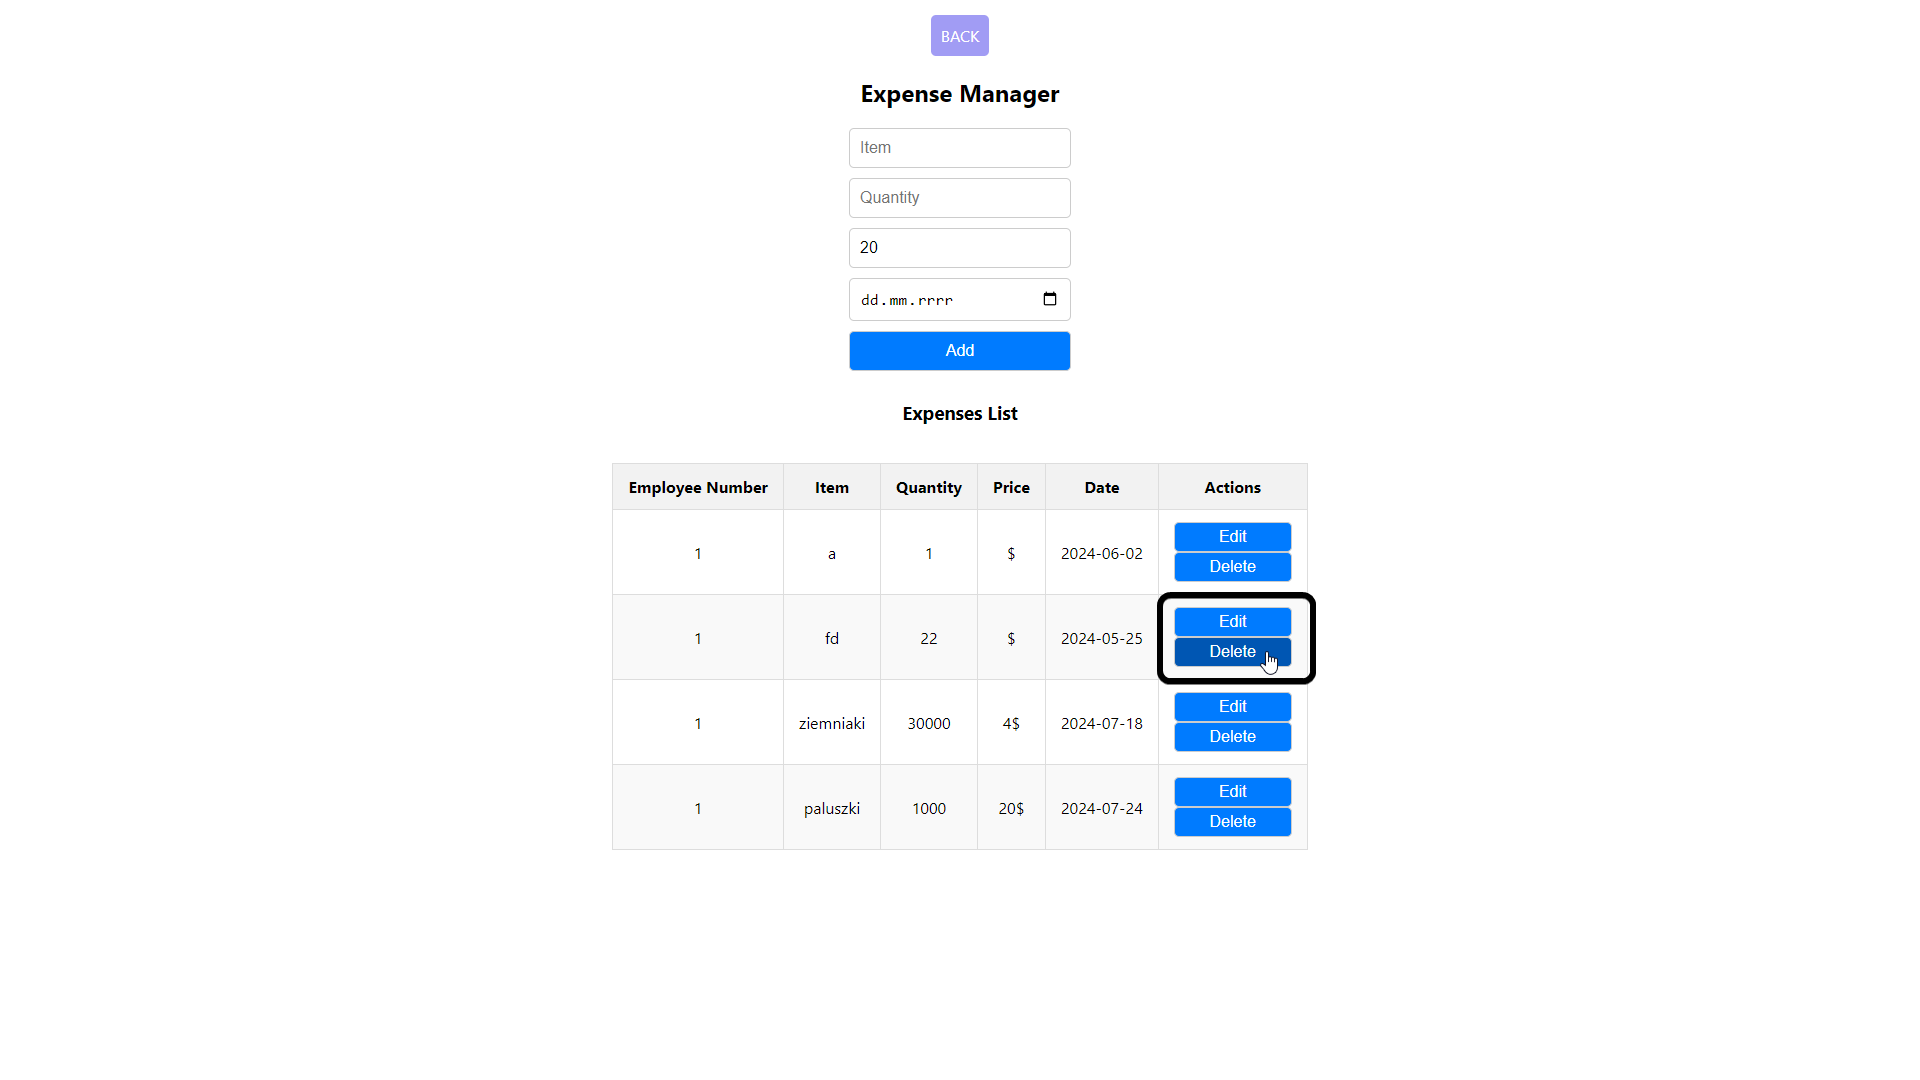
\includegraphics[width=\textwidth]{media/Expenses_delete.png}
\end{center}
\end{minipage}

\begin{minipage}{\textwidth}
\noindent Po wciśnięciu przycisku \textbf{Delete}, wydatek zostaje usunięty:
\begin{center}
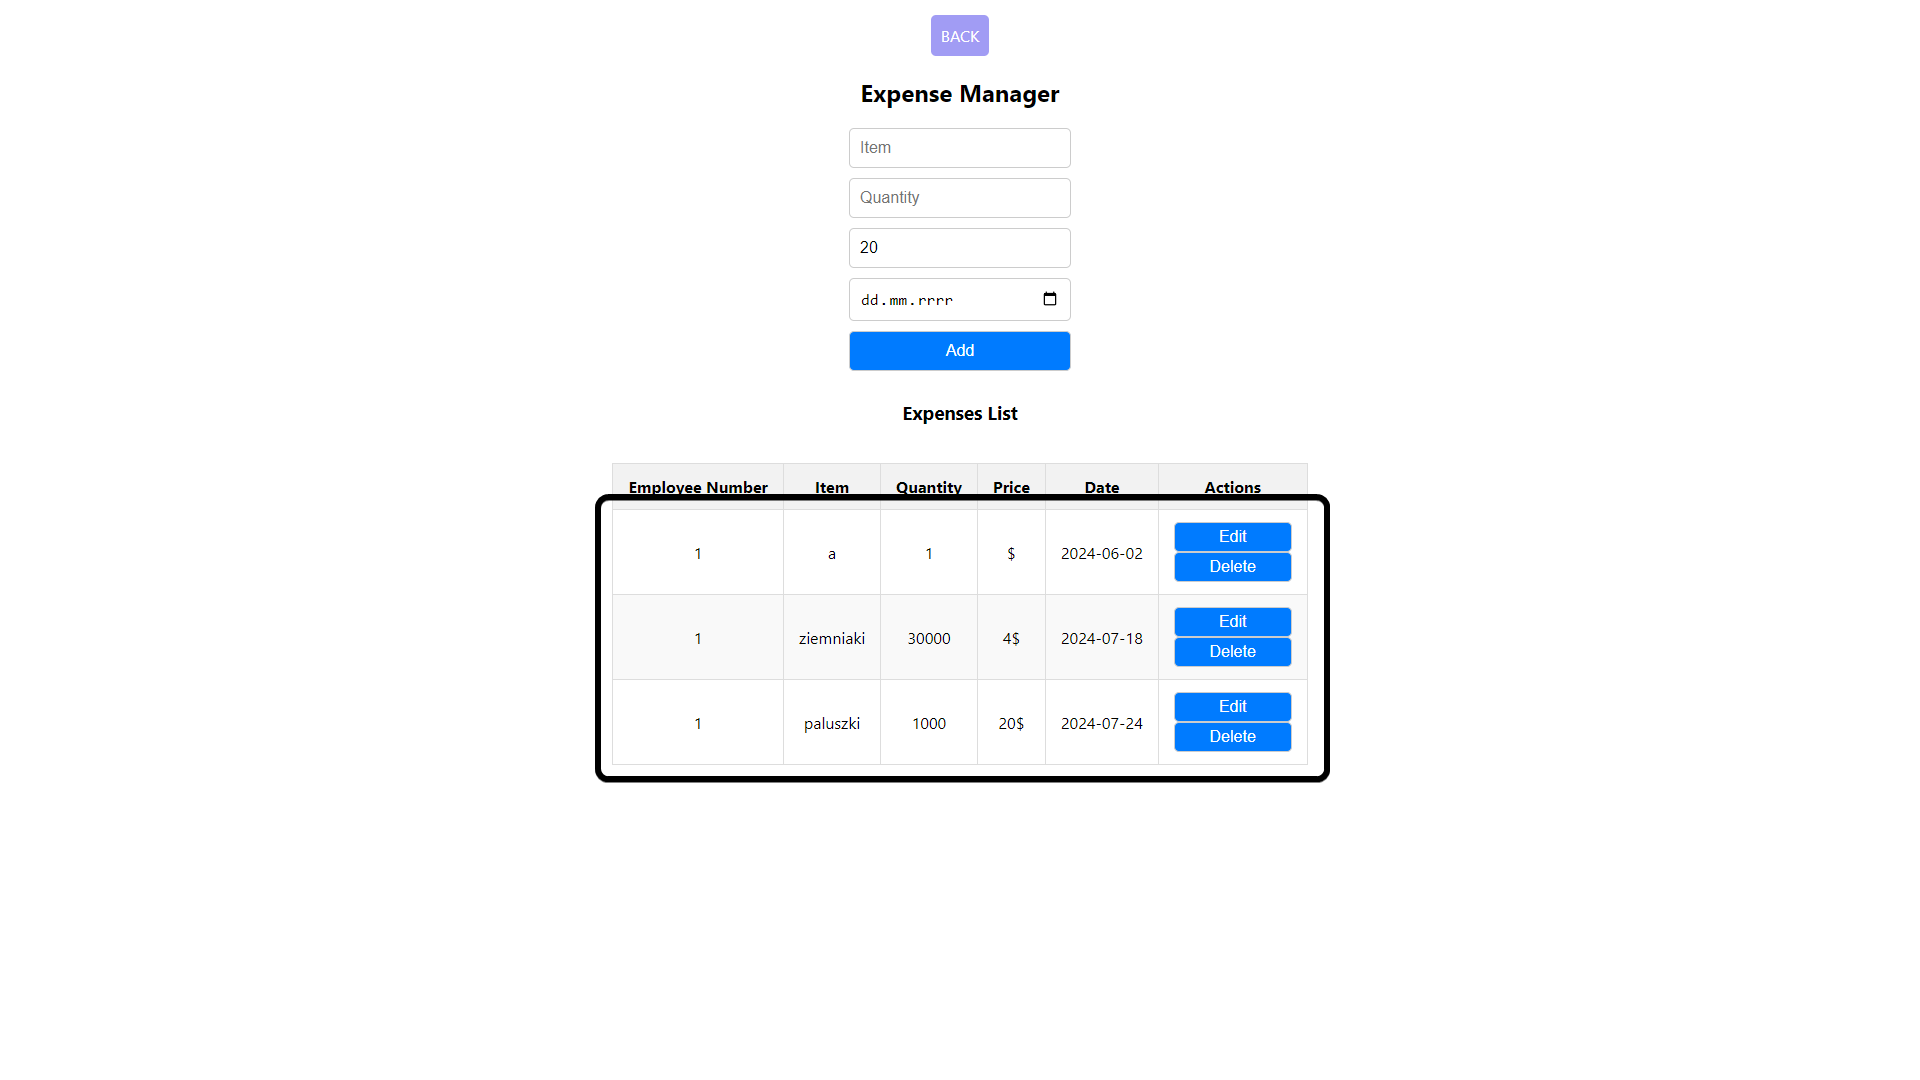
\includegraphics[width=\textwidth]{media/Expenses_deleteSuccessfull.png}
\end{center}
\end{minipage}

\newpage
\subsection{Incomes}
\begin{minipage}{\textwidth}
\noindent Po wciśnięciu przycisku \textbf{Incomes}:
\begin{center}
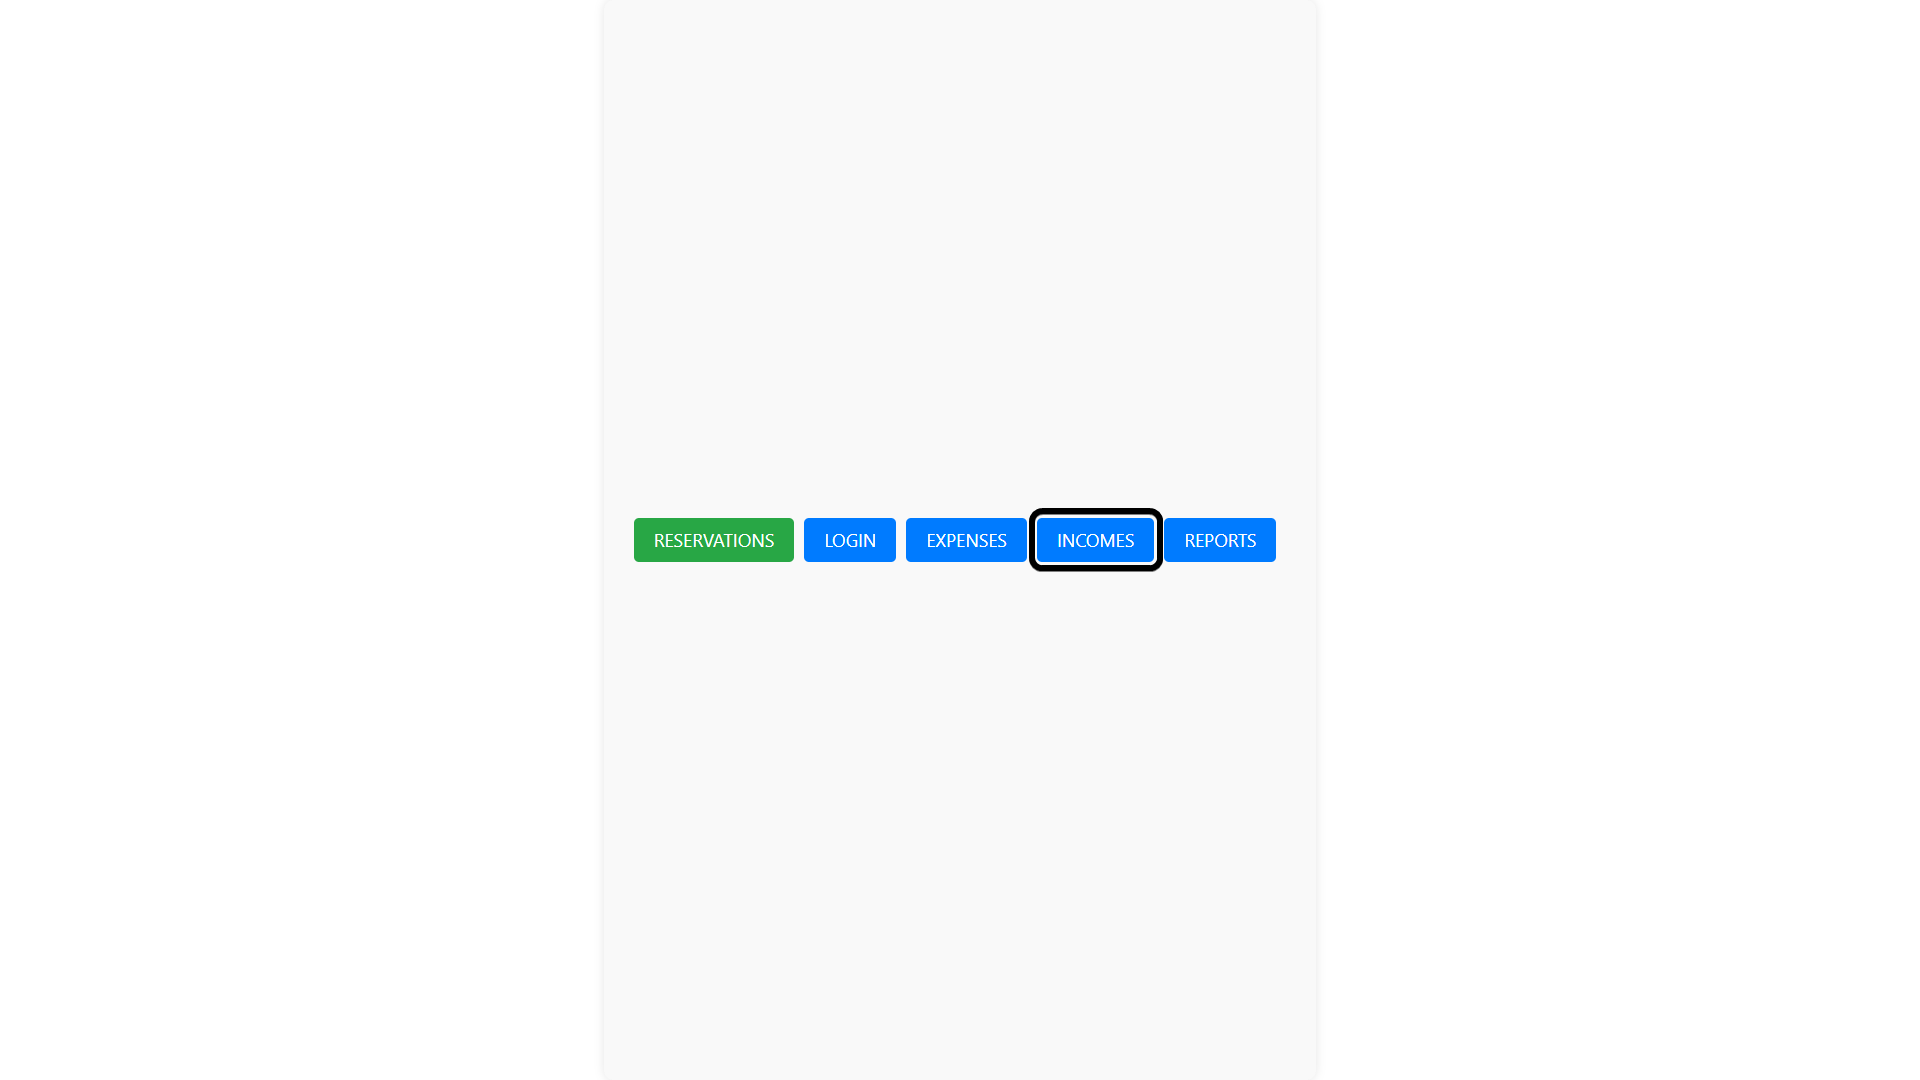
\includegraphics[width=\textwidth]{media/Incomes.png}
\end{center}
\end{minipage}

\begin{minipage}{\textwidth}
\noindent Przenosimy się do panelu wpływów:
\begin{center}
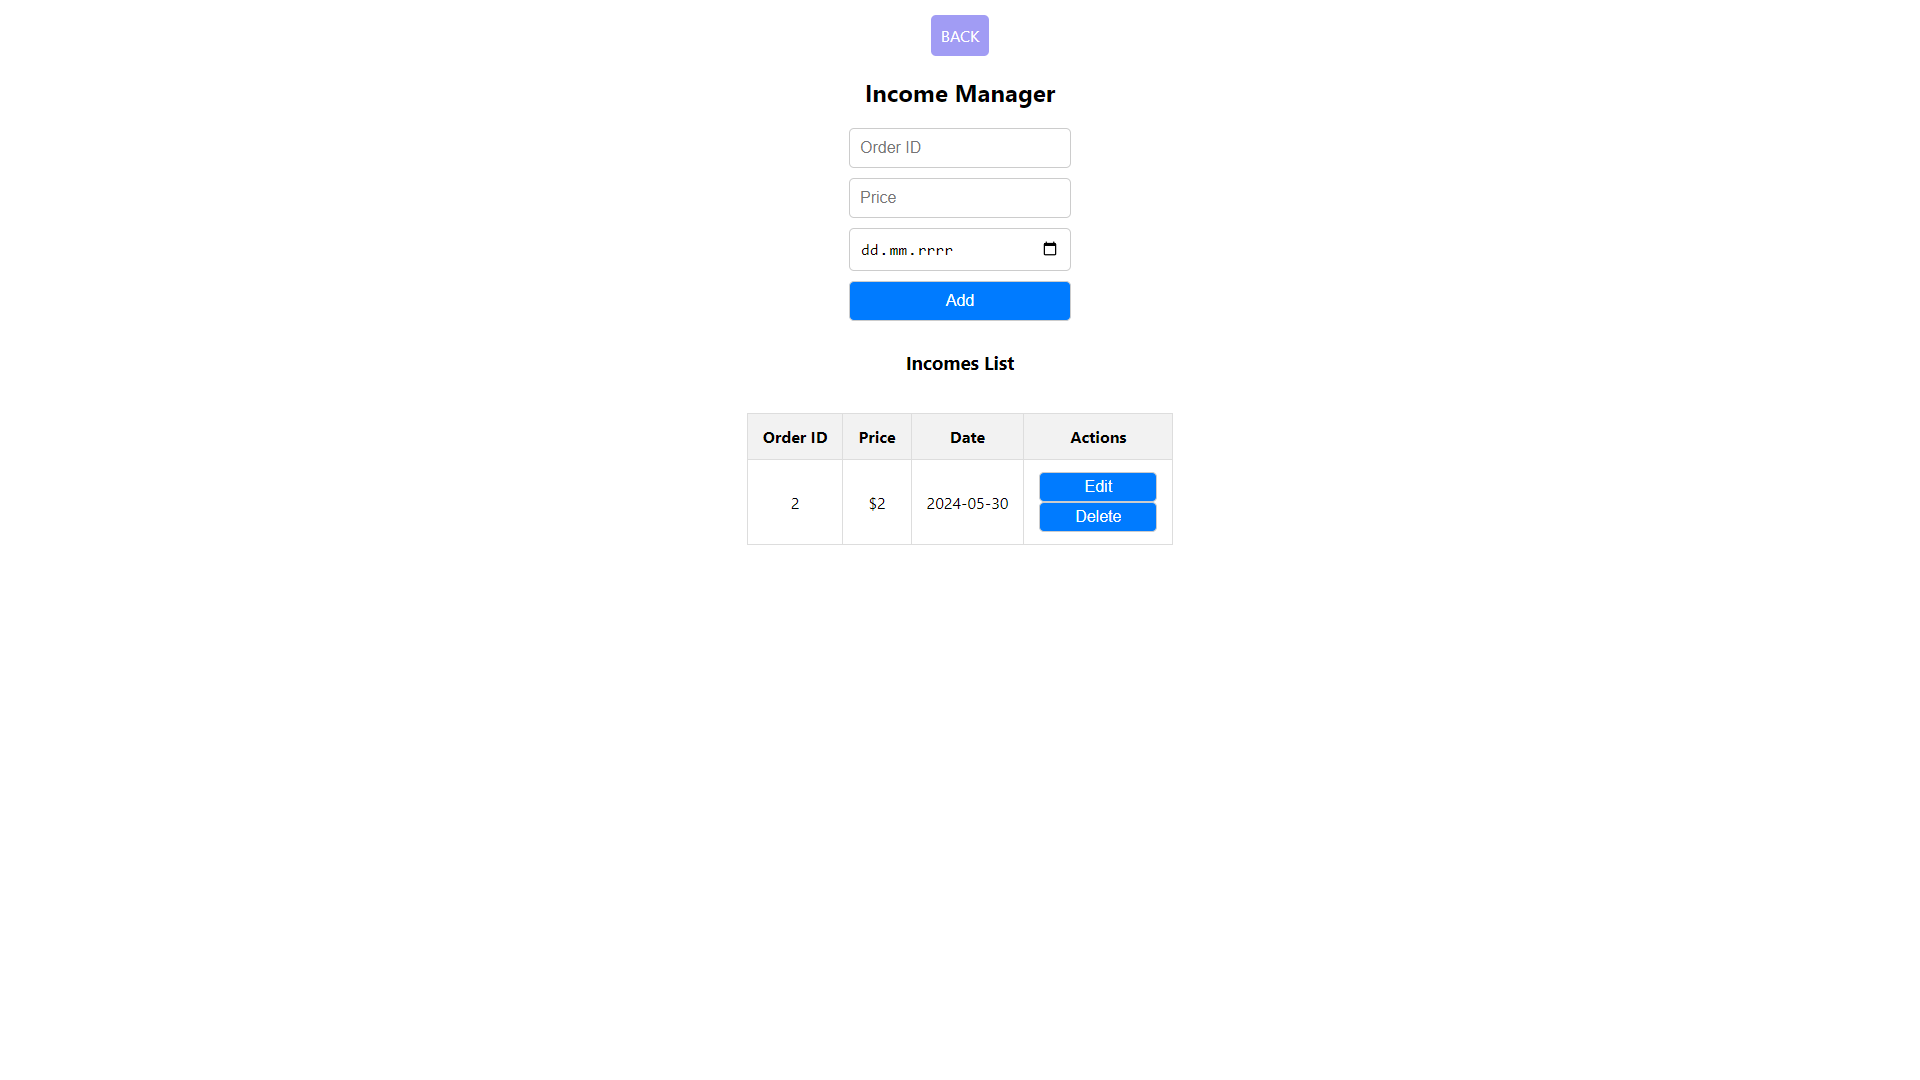
\includegraphics[width=\textwidth]{media/Incomes_in.png}
\end{center}
\end{minipage}

Panel wpływów oferuje takie same funkcjonalności, jak panel wydatków i jego obsługa jest taka sama.

\newpage
\subsection{Report}
\begin{minipage}{\textwidth}
\noindent Po wciśnięciu przycisku \textbf{Report}:
\begin{center}
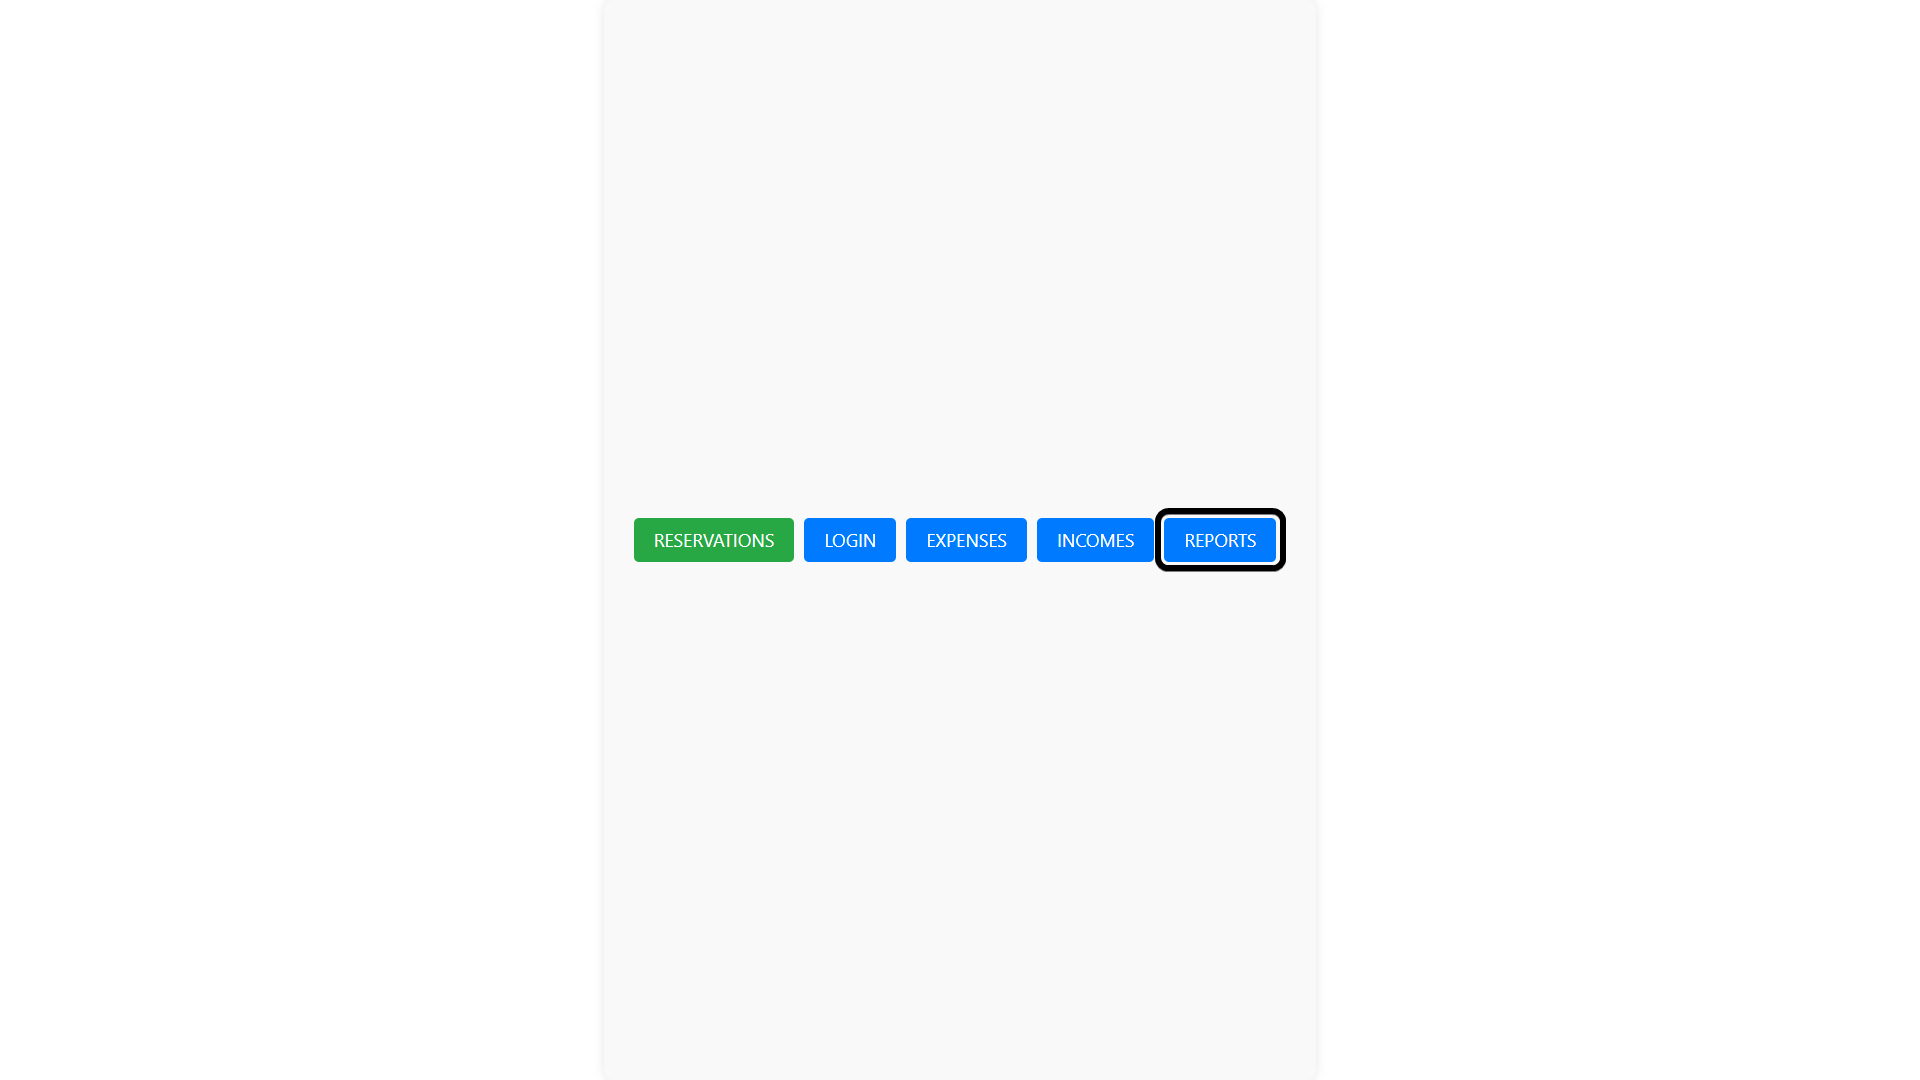
\includegraphics[width=\textwidth]{media/Reports.png}
\end{center}
\end{minipage}

\begin{minipage}{\textwidth}
\noindent Przenosimy się do panelu, gdzie mamy możliwość podglądu wygenerowanego raportu:
\begin{center}
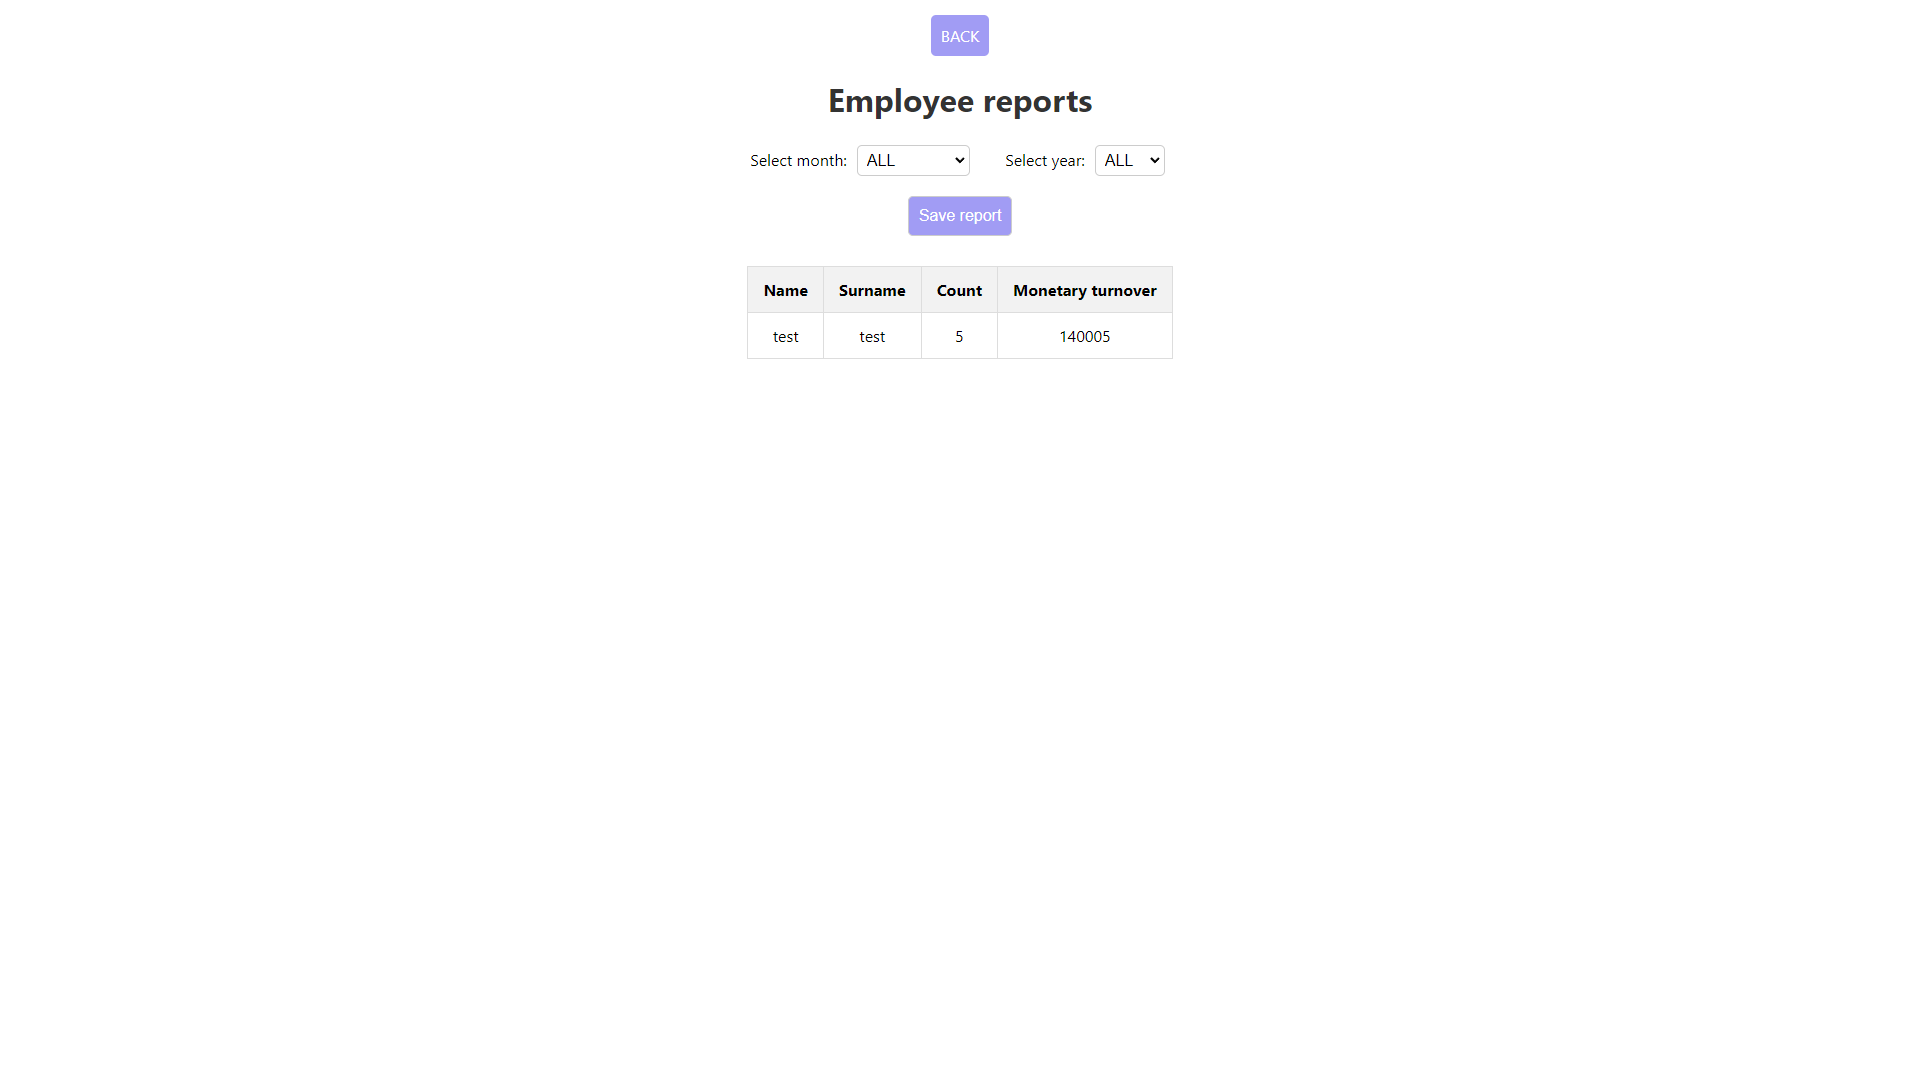
\includegraphics[width=\textwidth]{media/Report_in.png}
\end{center}
\end{minipage}

\begin{minipage}{\textwidth}
\noindent Mamy możliwość sprecyzowania, z którego miesiąca chcemy wygenerować raport (albo ze wszystkich, opcja \textbf{ALL}):
\begin{center}
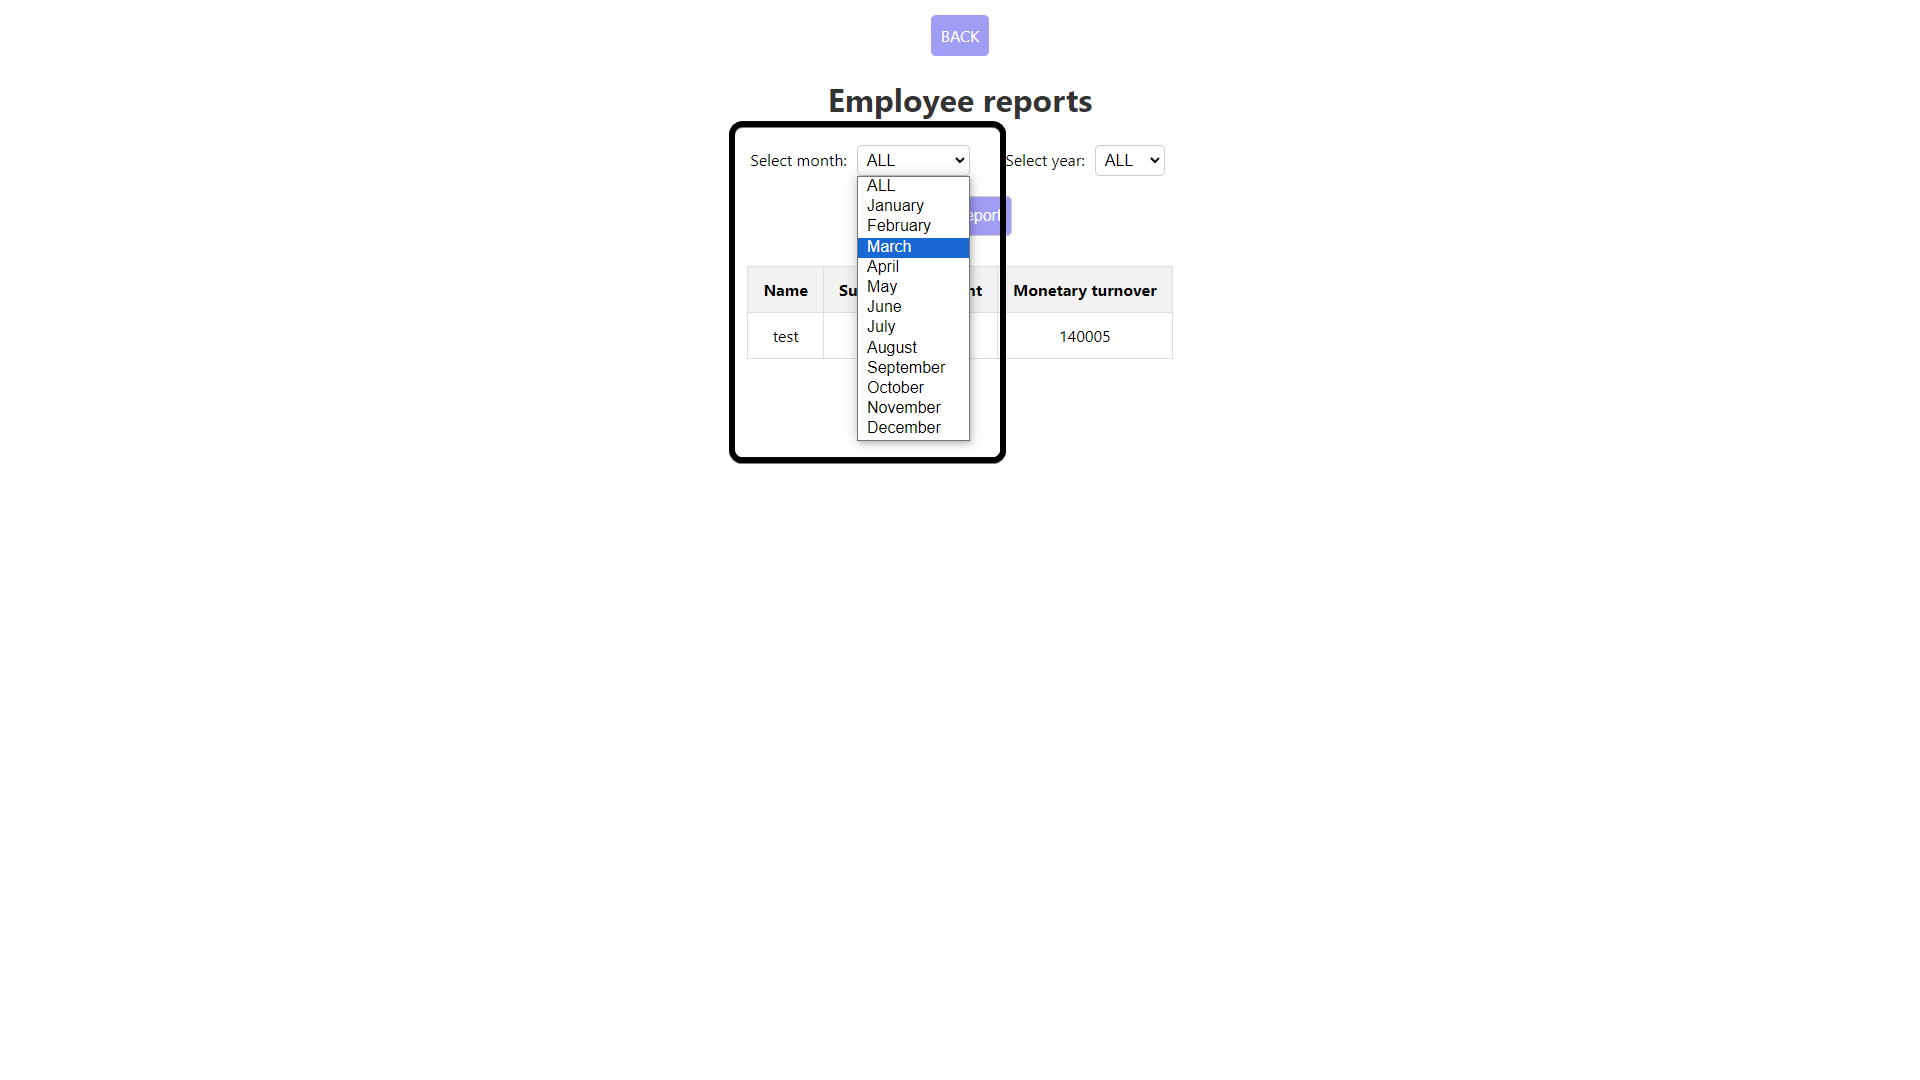
\includegraphics[width=\textwidth]{media/Report_month.png}
\end{center}
\end{minipage}

\begin{minipage}{\textwidth}
\noindent Tak jak i analogiczną możliwość sprecyzowania roku:
\begin{center}
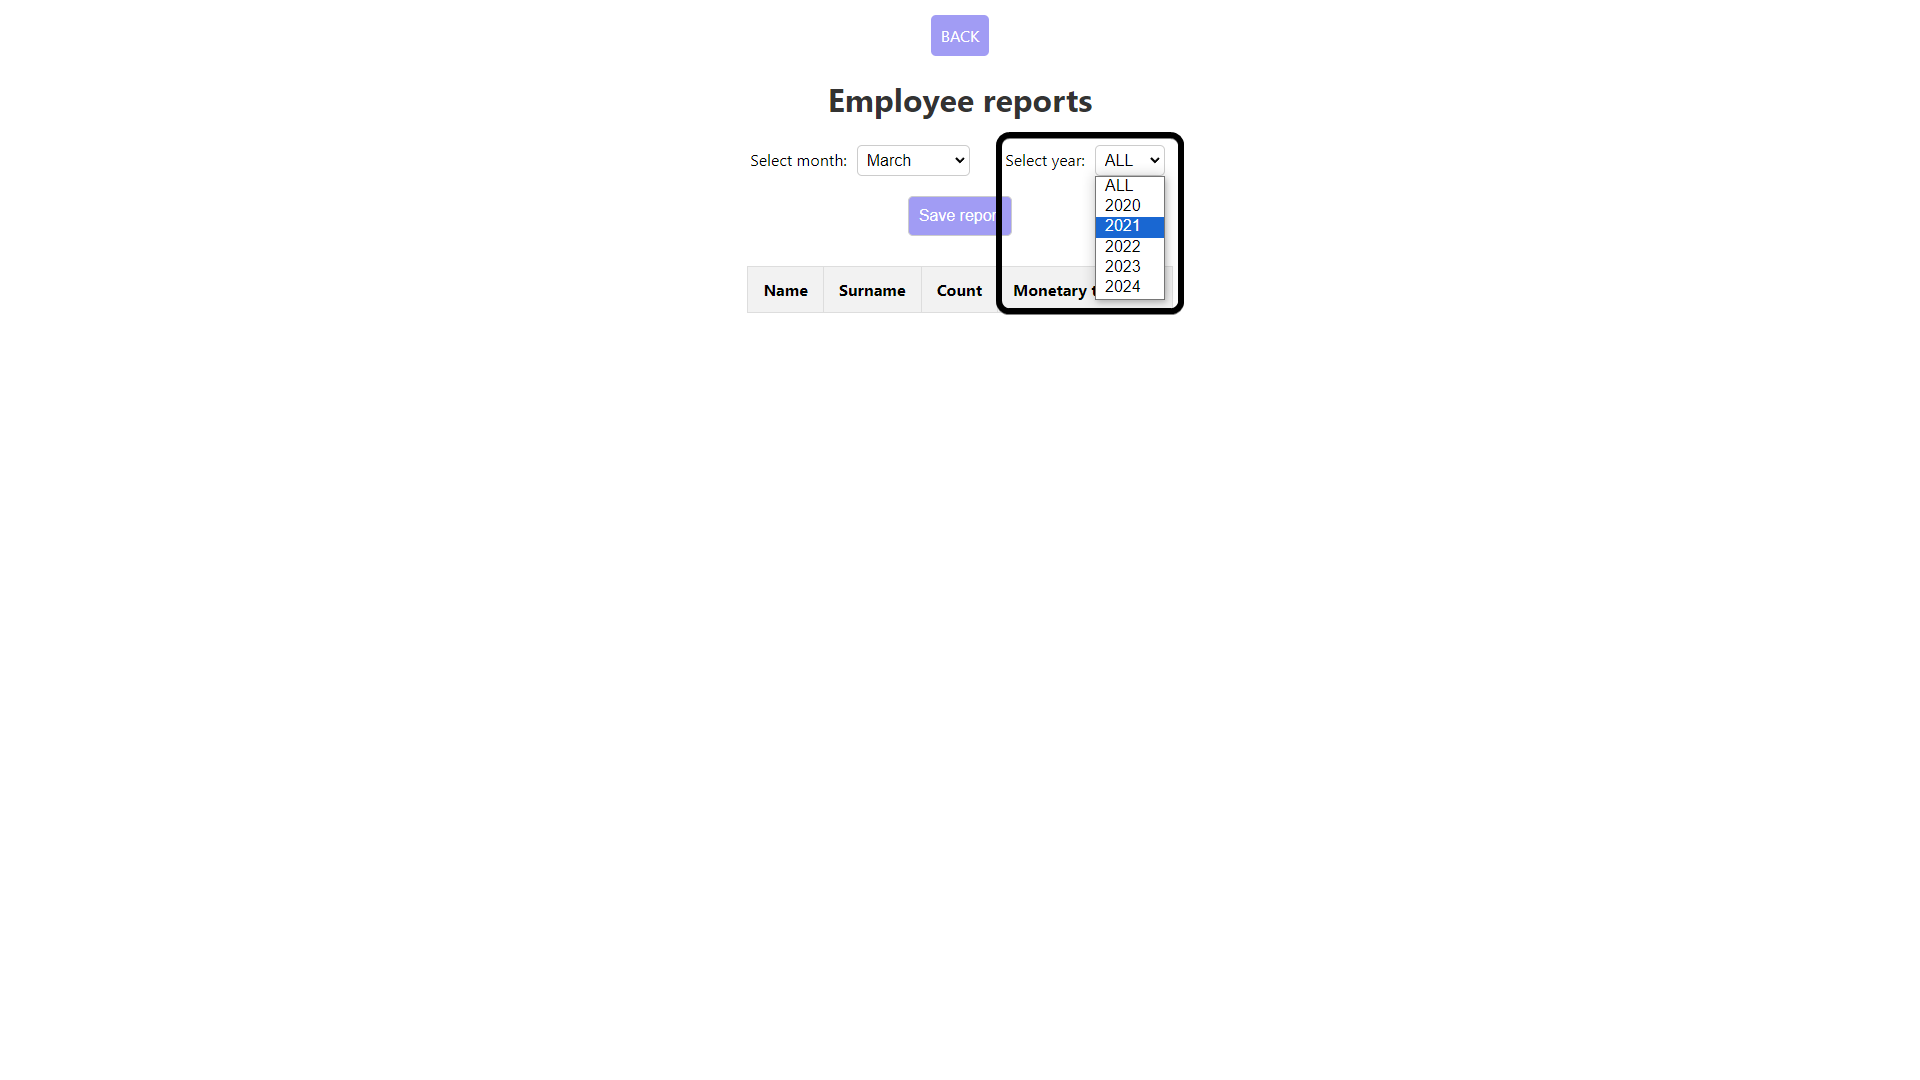
\includegraphics[width=\textwidth]{media/Reports_year.png}
\end{center}
\end{minipage}

\begin{minipage}{\textwidth}
\noindent Mamy również możliwość zapisania wyników raportu do pliku csv, za pomocą przysku \textbf{Save}:
\begin{center}
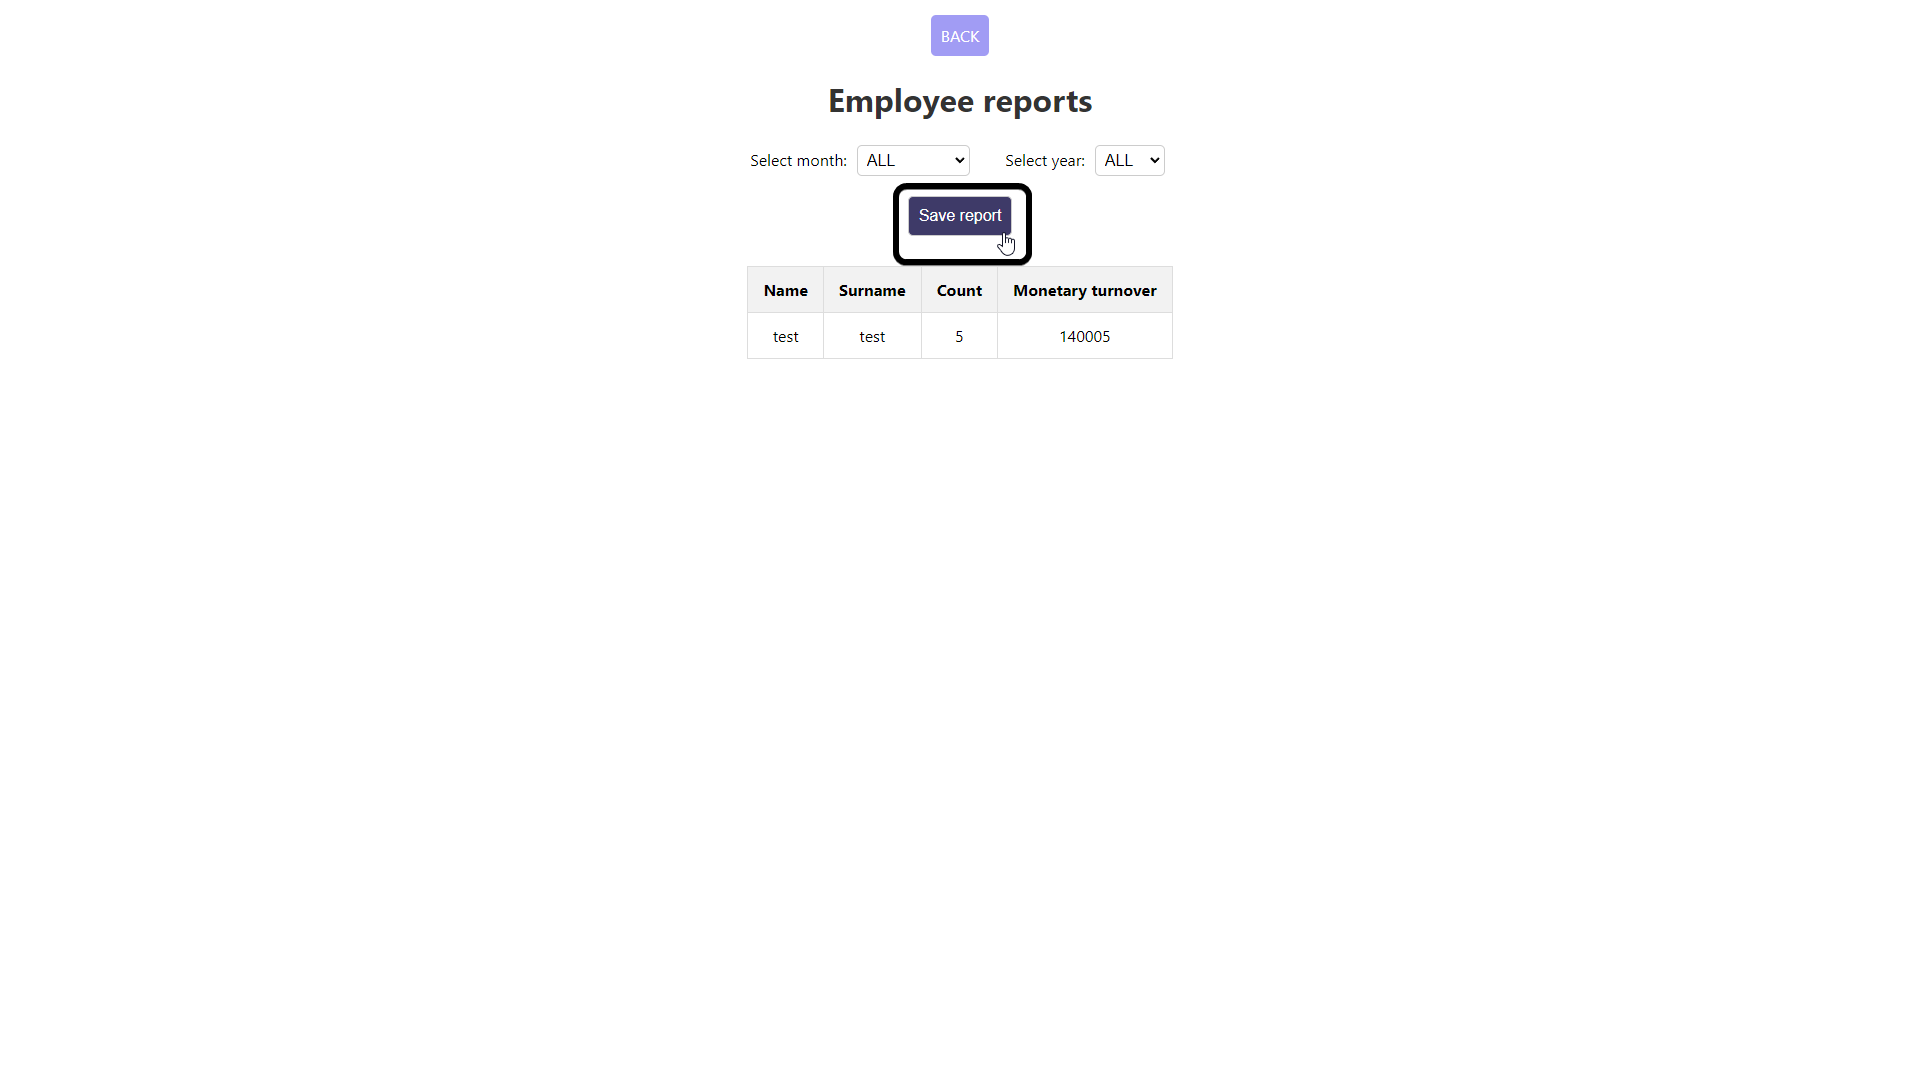
\includegraphics[width=\textwidth]{media/Reports_save.png}
\end{center}
\end{minipage}

\begin{minipage}{\textwidth}
\noindent Po jego wciśnięciu, dostajemy komunikat:
\begin{center}
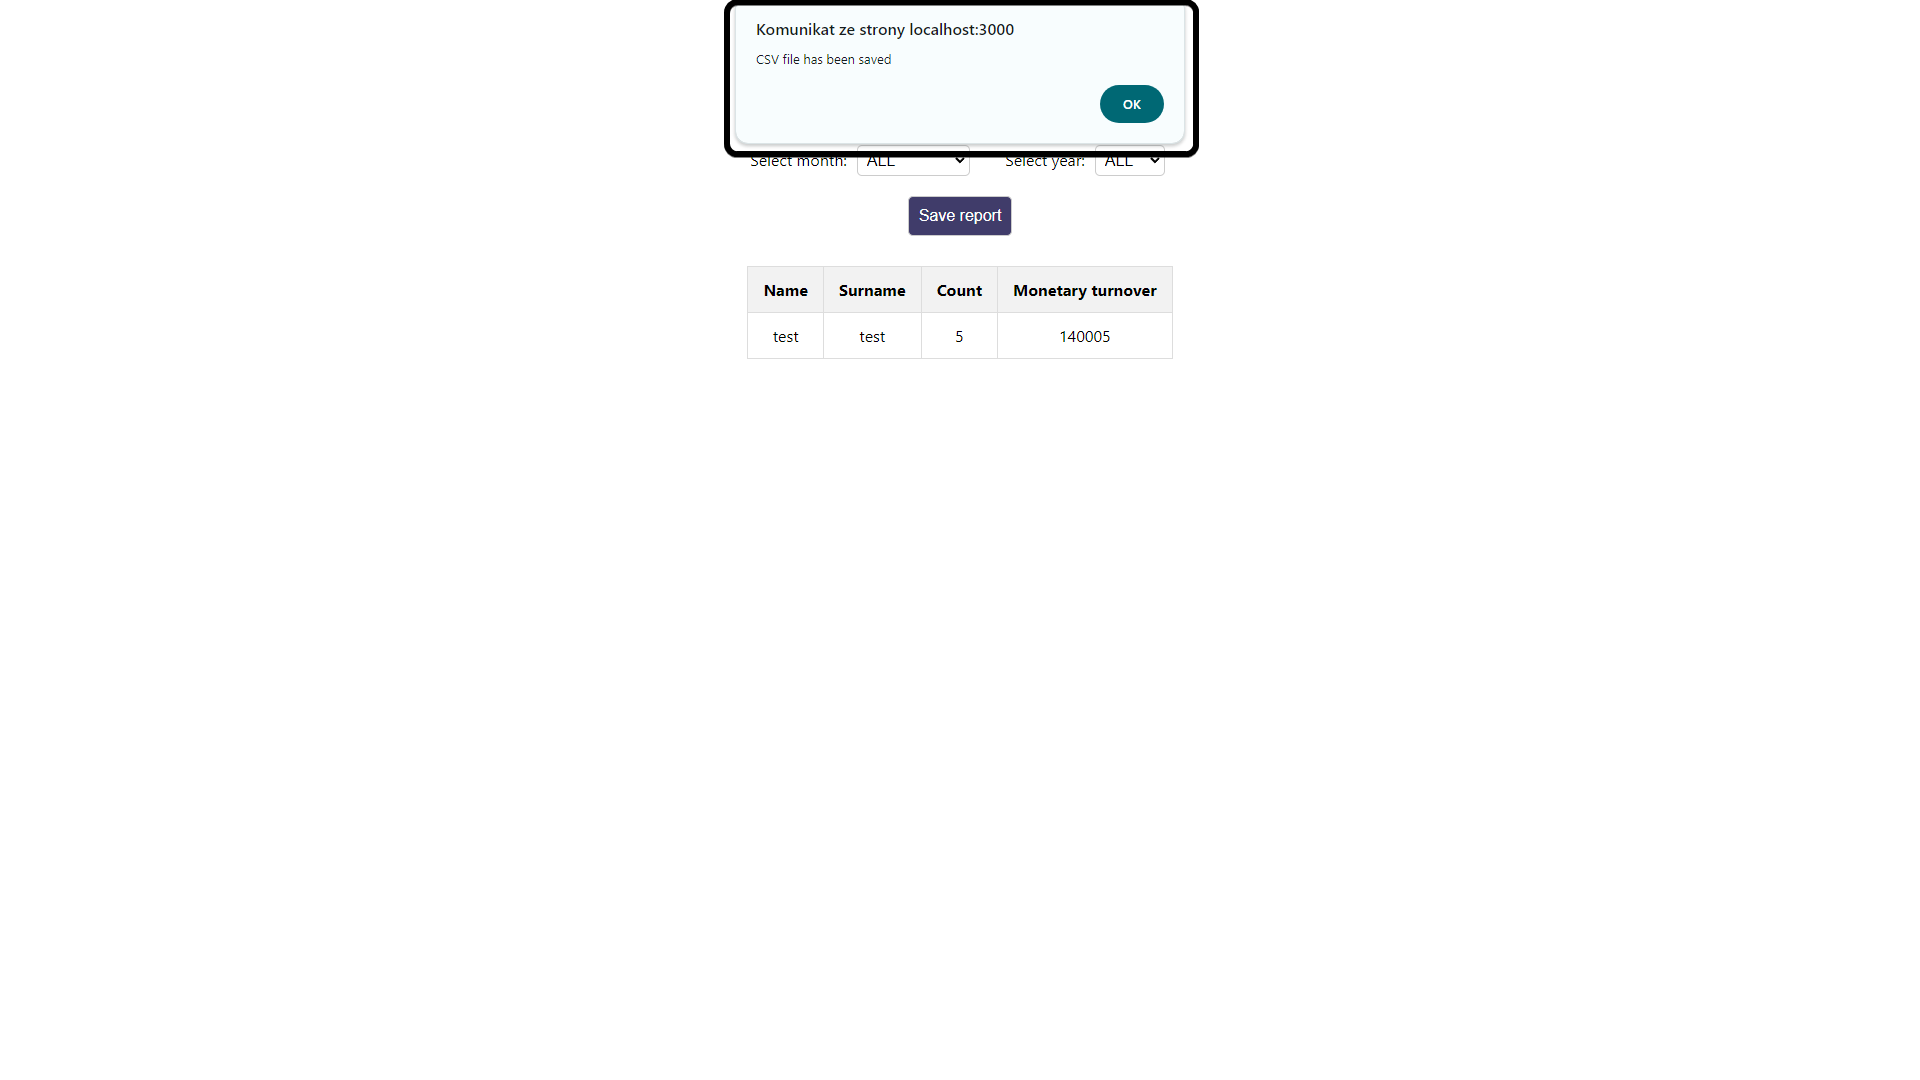
\includegraphics[width=\textwidth]{media/Reports_saved.png}
\end{center}
\end{minipage}

\newpage
\subsection{Niezalogowany pracownik}
\begin{minipage}{\textwidth}
\noindent Jeśli pracownik nie zaloguje się na żadne konto, nie będzie miał on dostępu do funkcjonalności oprogramowania:
\begin{center}
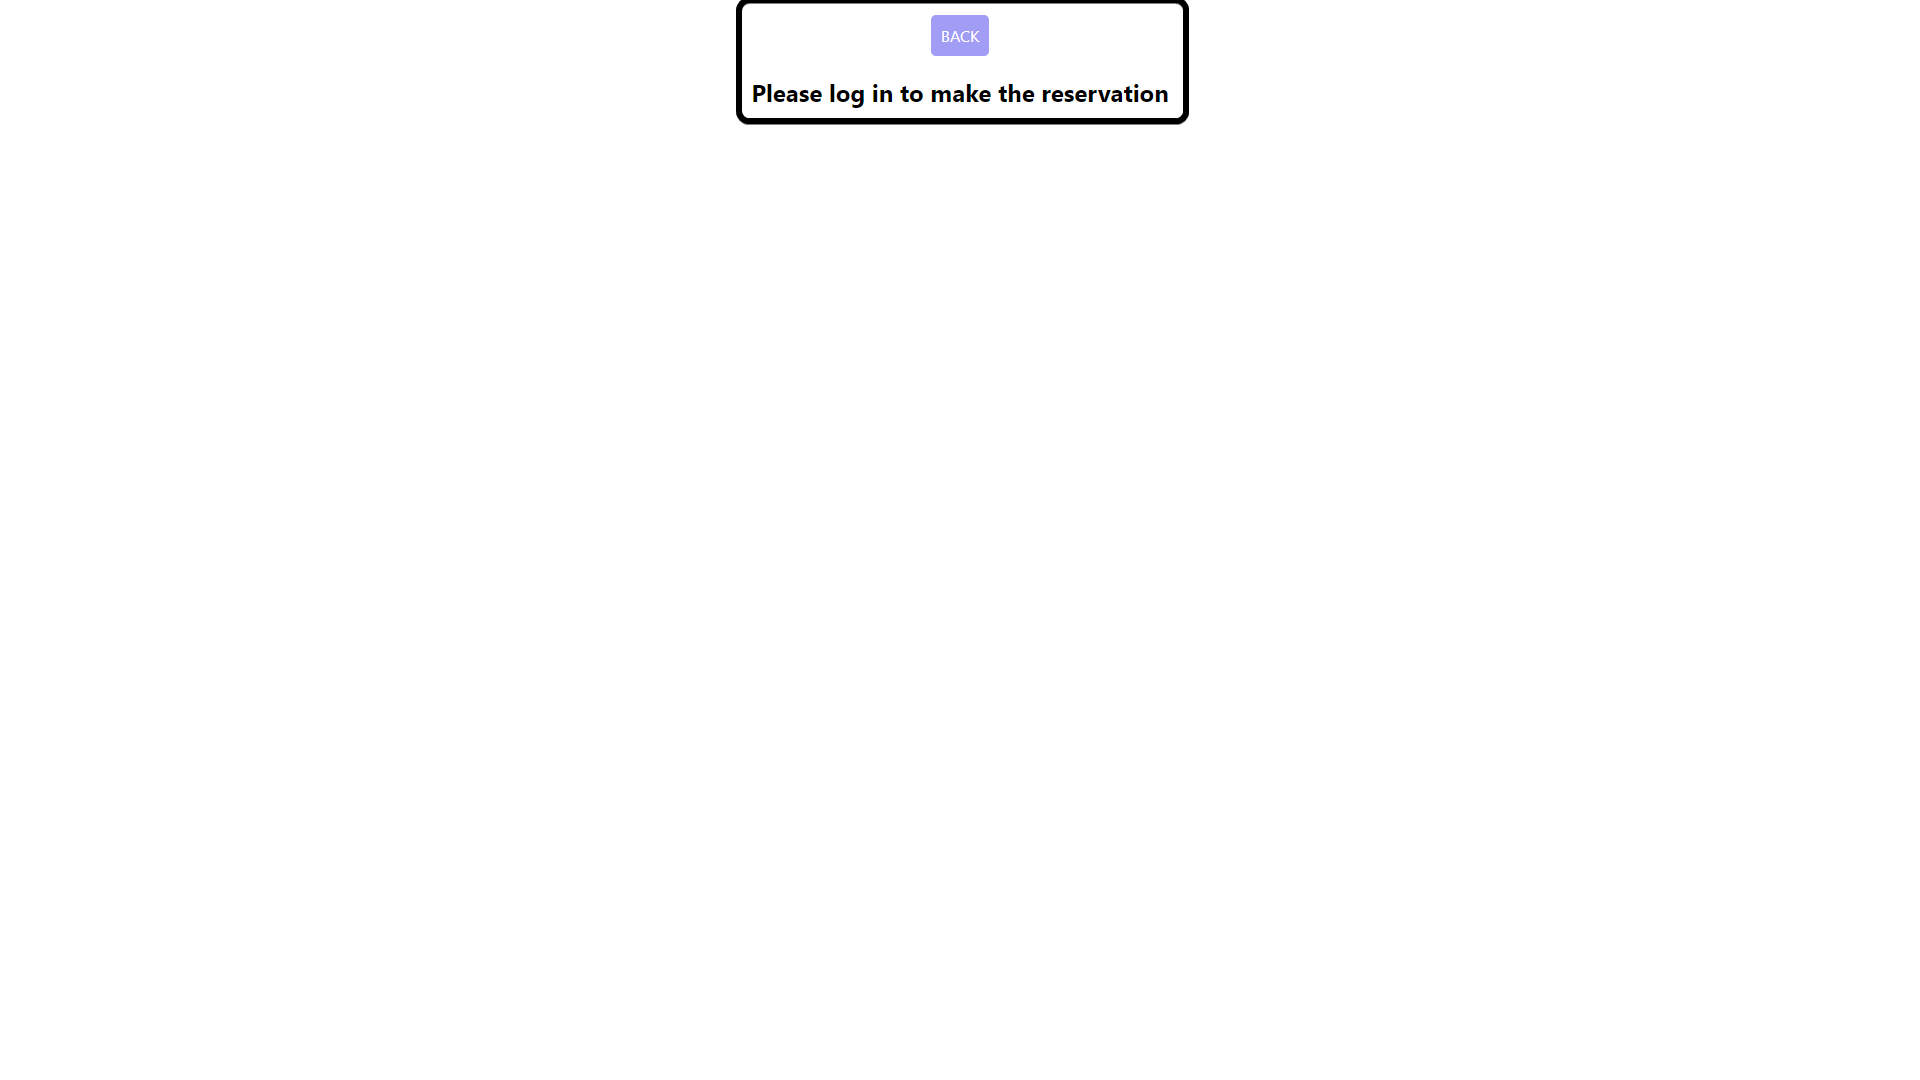
\includegraphics[width=\textwidth]{media/NotLoggenIn.png}
\end{center}
\end{minipage}

\newpage
\section{Dyskusja zrealizowanych technik}

\subsection{Trigger przy dodawaniu nowej rezerwacji}
Podczas dodawania nowej rezerwacji, by nie przechowywać zbędnych starych rezerwacji, usuwane są wszystkie rezerwacje, których data jest wcześniejsza niż aktualny dzień. CleanReservations to funkcja, która odpowiada za wyszukanie i usunięcie starych rezerwacji
\begin{lstlisting}[caption={Trigger}]
	resSchema.post('save', function(doc) {
		cleanReservations();
	})
\end{lstlisting}

\subsection{Możliwość zapisu raportu}
Nasza aplikacja wspiera zapisywanie wygenerowanego raportu do pliku .csv, który można potem łatwo analizować i obrabiać. Zdecydowaliśmy się na to, ponieważ uważamy, że samo wyświetlanie się danych nie byłoby wystarczające dla klienta i na pewno takie usprawnienie zwiększa wygodę używania aplikacji.

\end{document}